\documentclass[aps,prd,twocolumn,amsmath,amssymb]{revtex4-2}

\usepackage{graphicx}
\usepackage{mathtools}
\usepackage{braket}
\usepackage{cancel}
\usepackage{xcolor}

% Macros carried over from the thesis
\providecommand{\texorpdfstring}[2]{#1}
\newcommand{\tAmp}{\widetilde{A}}
\newcommand{\tBmp}{\widetilde{B}}
\newcommand{\Amp}{\ensuremath{A^{(+)}}}
\newcommand{\Bmp}{\ensuremath{B^{(+)}}}
\newcommand{\vect}[1]{\ensuremath{\boldsymbol{#1}}}
\newcommand{\vprp}[1]{\vect{#1}_{\mathrm T}}
\newcommand{\tcdot}{{\cdot}}
\newcommand{\bvec}{b}
\newcommand{\elll}{b}
\newcommand{\kei}{k}
\newcommand{\mN}{m_N}
\newcommand{\zetahat}{{\hat \zeta}}
\newcommand{\unsub}{\text{unsubtr.}}
\newcommand{\GammaOp}{\Gamma}
\newcommand{\myeps}{\ensuremath{\epsilon}}
\newcommand{\softf}{\mathcal{S}}
\newcommand{\fourint}{\ensuremath{\int_\mathcal{F}}}
\newcommand{\toddmark}[1]{\ensuremath{\Bigg[#1\Bigg]_{\text{\tiny{odd}}}}}
\newcommand{\Wline}[1]{\ensuremath{{\mathcal{U}}[#1]}}
\newcommand{\WlineC}[1]{\ensuremath{{\mathcal{U}}{[#1]}}}
\newcommand{\U}{\mathcal{U}{[\mathcal{C}_{b}]}}
\newcommand{\nminus}{\ensuremath{n}}
\newcommand{\nucl}[1]{{#1}}
\newcommand{\quark}{q}
\newcommand{\prp}{\perp}

\begin{document}

\title{Dependence of the Sivers TMD Shift on Quark Longitudinal Momentum Fraction $x$ from Lattice QCD}

\author{Hariprashad Ravikumar}
\author{Michael Engelhardt}
\affiliation{Department of Physics, New Mexico State University, Las Cruces, NM 88003, USA}

\date{\today}

\begin{abstract}
We compute the dependence of the isovector ($u-d$) Sivers shift on the quark longitudinal momentum fraction $x$ in lattice QCD with 2+1 flavors of clover-improved Wilson fermions at a lattice spacing of $a=0.11403$~fm and a pion mass of $m_\pi=317$~MeV. The transverse momentum dependent parton distributions (TMDs) are defined through quark bilinears with staple-shaped Wilson lines. The generalized Sivers shift $\langle k_y\rangle_{TU}=m_N\,\tilde f_{1T}^{\perp(1)}/\tilde f_1^{(0)}$, the ratio of the Sivers TMD to the unpolarized TMD, is obtained from a ratio of Lorentz-invariant amplitudes. To extract the $x$-dependence, we scan the full accessible range of $b\cdot P$, the variable Fourier conjugate to $x$. This requires staples along off-axis lattice directions, which we obtain by interpolation.
Using the PySR symbolic regression and statistical modeling, we systematically explored several ans\"atze that satisfy physical constraints, and we describe the amplitudes at four nucleon momenta with a global fit in $b\cdot P$, $b^2$, and the staple length $\eta$. After extrapolation to the light-cone limit $\hat\zeta\to\infty$, the magnitude of the $x$-weighted isovector Sivers shift $x\langle k_y\rangle_{TU}$ at $|\vect{b}_T|=0.34$~fm, for SIDIS/DY, is about $0.006$--$0.011$~GeV for $0.3\le x\le 0.4$. For $0.34\le|\vect{b}_T|\le 0.94$~fm, the isovector Sivers shift is close to, but not exactly, a product of a function of $x$ and a function of $|\vect{b}_T|$, with a relative distance of 6--8\% from the best factorized form.
\end{abstract}

\maketitle

\section{Lattice Setup}
\label{sec:setup}
All results are for the isovector $u-d$ combination on a single $32^3\times96$ ensemble with 2+1 flavors of clover-improved Wilson fermions, generated by the JLab/W\&M collaboration, with $a=0.11403(77)$~fm and $m_\pi=317(2)(2)$~MeV. The ensemble has 968 configurations. On each configuration we compute proton and antiproton propagators from 12 source positions each, together with the corresponding sequential propagators, which gives $968\times24=23232$ measurements. We divide these into blocks of 8 and form 2902 jackknife sets after discarding a few faulty samples. The nucleon mass is $m_N=0.6228(28)/a=1077.8(48)$~MeV. The momentum transfer is zero, and the sink momentum is $\vect{P}=(2\pi/\hat L a)(n,0,0)$ with $n=-1,-2,-3,-4$ and $\hat L=32$. We use $t_{\rm src}=0$ and $t_{\rm snk}=t_{\rm sep}=10$.
% TODO(Hari): the thesis does not state the smearing of the nucleon source/sink; add it here if it should be reported.

\section{Formalism}
\label{sec:formalism}
\subsection{Definition of TMDs}
\label{sec:tmd_definition}
Consider a frame of reference where the nucleon has large momentum in the $z$-direction, i.e., $P^+ \gg m_N$, $\vprp{P} = 0$.
In light cone coordinates, the components $\kei^+$,~$\vprp{\kei}$,~$\kei^-$ of the quark momentum $\kei$ scale as $P^+/m_N$,~$1$,~$m_N/P^+$, respectively, under boosts along the $z$-axis. Thus, the quark longitudinal momentum fraction $x = k^+ / P^+$ and the transverse momentum $\vprp{\kei}$ are invariant under boosts along the $z$-axis, while the $k^-$ component is suppressed. 
This leads to transverse momentum-dependent parton distribution functions (TMDs), which depend on the longitudinal momentum fraction $x \equiv \kei^+ / P^+$ and the quark transverse momentum $\vprp{\kei}$. 
The transverse momentum components $\vprp{\kei}$ describe an intrinsic motion of the quarks inside the proton that occurs independently of the momentum of the proton itself. TMDs are an important ingredient for understanding the origin of the large angular and spin asymmetries observed in experiments such as semi-inclusive deep inelastic scattering (SIDIS) and the Drell-Yan process (DY).

We construct a correlator from the gauge-invariant bilocal operator $\bar q(0) \Gamma \WlineC{\mathcal{C}_\bvec} q(\bvec)$ acting on the nucleon state $\ket{P, S}$, where $\bar q$ and $q$ are local quark field operators, and the Wilson line $\WlineC{\mathcal{C}_\bvec}$ makes the bi-local operator gauge invariant. The Fourier transform of such a position space correlator $\bra{P,S}\ \bar{q}(0)\, \Gamma\ \WlineC{\mathcal{C}_\bvec}\ q(\bvec)\ \ket{P,S}$ with respect to $b$ gives the momentum space correlator $\Phi^{[\Gamma]}(\kei,P,S;\ldots)$, or equivalently the TMDs. The Wilson
line (to be specified in more detail below) introduces divergences that conventional dimensional
regularization cannot treat~\cite{Musch:2011er}, so we divide by the soft factor, $\widetilde{\softf}(\bvec^2;\ldots)$, 
\begin{widetext}
\begin{align}
	\Phi^{[\Gamma]}(\kei,P,S;\ldots)\ \equiv\ \ 
	\int \frac{d^4 \bvec}{(2\pi)^4}\, e^{i \kei\cdot \bvec}\,
		\frac{\overbrace{\rule{0em}{1.2em}
		\frac{1}{2}\, \bra{P,S}\ \bar{q}(0)\, \Gamma\ \WlineC{\mathcal{C}_\bvec}\ q(\bvec)\ \ket{P,S}
		}^{\displaystyle \equiv \widetilde \Phi_\unsub^{[\Gamma]}(\bvec,P,S;\ldots)}}
		{ \widetilde{\softf}(\bvec^2;\ldots) } \ .
		\label{eq-corr}	
\end{align}
\end{widetext}
The numerator, $\widetilde \Phi_\unsub^{[\Gamma]}(\bvec, P,S;\ldots)$, is the bare non-local matrix element in which a gauge link $\WlineC{\mathcal{C}_\bvec}$ connects the quark fields. The denominator is the soft factor, $\widetilde{\softf}(\bvec^2;\ldots)$, which regulates rapidity divergences. The ellipses (``$\ldots$'') denote additional dependence on parameters governing the Wilson line geometry and the soft factor, as well as an implicit dependence on the ultraviolet renormalization scale $\mu$.

The soft factor, $\tilde \softf$, stands symbolically for an
expression that can, depending on the formalism, involve several vacuum
expectation values. In the framework of Collins and Aybat~\cite{Aybat:2011zv,CollinsBook2011,Aybat:2011ge}, it takes the form
\begin{equation}
\widetilde{\softf}(\bvec^2;\ldots) = 
  \sqrt{ \frac
    { \tilde S_{(0)}( \vprp{\bvec}, + \infty, -\infty )\ \tilde S_{(0)}( \vprp{\bvec}, y_s, -\infty ) }
    { \tilde S_{(0)}( \vprp{\bvec}, + \infty, y_s ) }
  } \ ,
\end{equation}
here each of the objects $\tilde S_{(0)}( \vprp{\bvec}, \ldots )$ is a
vacuum expectation value of Wilson line structures.
In this framework, we start with space-like Wilson lines. Some Wilson lines remain tilted away from the light cone, leading to the dependence on the rapidity parameter $y_s$ in the above expression. We need not specify $\tilde \softf$ further, since it cancels in the observables we consider.

To project the correlator onto the relevant kinematics, we integrate over the suppressed momentum component $k^-$, which sets the position-space separation to $b^+ = 0$:
\begin{widetext}
\begin{align}
	\Phi^{[\Gamma]}(x,\vprp{k};P,S;\ldots) & \equiv \int dk^{-} \Phi^{[\Gamma]}(\kei,P,S;\ldots) \nonumber \\ 
 &=\int dk^{-}\int \frac{d^4 \bvec}{(2\pi)^4}\, e^{i \kei\cdot \bvec} \frac{\frac{1}{2}\, \bra{P,S}\ \bar{q}(0)\, \Gamma\ \WlineC{\mathcal{C}_\bvec}\ q(\bvec)\ \ket{P,S}}{ \widetilde{\mathcal{S}}(-\vprp{\bvec}^2;\ldots) }\\
 &=\int dk^{-}\int \frac{db^{+}}{2\pi}e^{ik^-b^+}\int \frac{d^2\textbf{b}_T}{(2\pi)^2}\int \frac{db^-}{2\pi}e^{ik^+b^--i\textbf{k}_T\tcdot\textbf{b}_T}\frac{\frac{1}{2}\, \bra{P,S}\ \bar{q}(0)\, \Gamma\ \WlineC{\mathcal{C}_\bvec}\ q(\bvec)\ \ket{P,S}}{ \widetilde{\mathcal{S}}(-\vprp{\bvec}^2;\ldots) }\\
 &=\int {db^{+}}\delta(b^+)\int \frac{d^2\textbf{b}_T}{(2\pi)^2}\int \frac{db^-}{2\pi}e^{ik^+b^--i\textbf{k}_T\tcdot\textbf{b}_T}\frac{\frac{1}{2}\, \bra{P,S}\ \bar{q}(0)\, \Gamma\ \WlineC{\mathcal{C}_\bvec}\ q(\bvec)\ \ket{P,S}}{ \widetilde{\mathcal{S}}(-\vprp{\bvec}^2;\ldots) }\\
	& =\int \frac{d^2 \vprp{\bvec}}{(2\pi)^2} \int \frac{d (\bvec \tcdot P)}{(2\pi) P^+}\ e^{i x (\bvec \tcdot P) - i\vprp{\bvec} \tcdot \vprp{\kei}}\,
		\left. \frac{\frac{1}{2}\, \bra{P,S}\ \bar{q}(0)\, \Gamma\ \WlineC{\mathcal{C}_\bvec}\ q(\bvec)\ \ket{P,S}}
		{ \widetilde{\mathcal{S}}(-\vprp{\bvec}^2;\ldots) } \right|_{b^+ = 0} \ .
\end{align}
\end{widetext}
As a consequence, $x \leftrightarrow (\bvec \tcdot P)$ and $\vprp{k} \leftrightarrow \vprp{b}$ are independent pairs of Fourier conjugate variables.
With the Dirac matrix $\Gamma = \gamma^+$, which projects onto the leading-twist unpolarized quark distribution, the correlator becomes~\cite{Ralston:1979ys, Tangerman:1994eh,Mulders:1995dh,Goeke:2005hb}:
\begin{align}
	\Phi^{[\gamma^+]}(x,\vprp{k};P,S,\ldots) & = f_1 - \toddmark{\frac{\myeps_{ij}\, \vect{k}_{i}\, \vect{S}_{j}}{m_N}\ f_{1T}^\prp} \label{eq-phigammaplus}\ . 
\end{align}
The term enclosed in $[\ ]_\text{odd}$ isolates the naively time-reversal odd (T-odd) Sivers function $f_{1T}^\perp$~\cite{Sivers:1989cc}, which describes the distribution of unpolarized quarks inside a transversely polarized nucleon. The origin of this parametrization and the special role of T-odd TMDs become clear once we discuss the geometry of the gauge link path $\mathcal{C}_\bvec $ and symmetry transformation properties.
\subsection{TMDs in Fourier space}
\label{sec:tmd_fourier}
Our lattice method evaluates the $b$-dependent matrix elements $\widetilde \Phi_\unsub^{[\Gamma]}(\bvec,P,S;\ldots)$ introduced in Eq. \eqref{eq-corr}. It is therefore more direct and natural to state our results in terms of Fourier-transformed, $\vprp{b}$-dependent TMDs and their $\vprp{b}$-derivatives. For a generic TMD $f$, we define the Fourier transform and its derivatives:
\begin{widetext}
\begin{align}
	\tilde f(x, \vprp{\bvec}^2;\ldots) & \equiv \int  d^2 \vprp{\kei} \, e^{i \vprp{\bvec} \cdot \vprp{\kei} }\; f(x, \vprp{\kei}^2;\ldots)
		= 2\pi \int      d|\vprp{\kei}| |\vprp{\kei}|\ J_0(|\vprp{\bvec}||\vprp{\kei}|)\  f(x, {\vprp{\kei}^2};\ldots )\ , \label{eq-FTMD} \\
	\tilde f^{(n)}(x, \vprp{\bvec}^2\ldots ) & \equiv n!\left( -\frac{2}{\mN^2}\partial_{\vprp{\bvec}^2} \right)^n \ 
	\tilde f(x, \vprp{\bvec}^2;\ldots ) \nonumber \\
		& = \frac{ 2\pi \ n!}{(\mN^2)^n} \int  d |\vprp{\kei}| |\vprp{\kei}|\left( \frac{|\vprp{\kei}|}{|\vprp{\bvec}|}\right)^n J_n(|\vprp{\bvec}||\vprp{\kei}|)\  f(x, {\vprp{\kei}^2};\ldots )\ , \label{eq-dFTMD}
\end{align}
\end{widetext}
where $J_n$ are the Bessel functions of the first kind, as shown in Ref.~\cite{Boer:2011xd}; these Bessel-weighted quantities can be used to structure evolution equations.

In the formal limit $|\vprp{\bvec}| \rightarrow 0$, they reduce to the conventional $\vprp{\kei}$-moments:
\begin{align}
	\tilde f^{(n)}(x, 0;\ldots ) & = \int  d^2 \vprp{\kei} \left( \frac{\vprp{\kei}^2}{2 \mN^2 }\right)^n  f(x, \vprp{\kei}^2;\ldots ) \equiv  f^{(n)}(x)\ .
	\label{eq-btder2}
\end{align}
However, the first transverse moment of the Sivers function, $f_{1T}^{\perp(1)}(x)$, diverges without additional regularization, because the perturbatively calculable high-$\vprp{\kei}$ tails do not decay fast enough~\cite{Bacchetta:2008xw}. We therefore do not extrapolate to $\vprp{\bvec}=0$. At finite $|\vprp{\bvec}|$, the integrals converge, and we access the $x$-dependence of the Sivers TMD through the conjugate variable $\bvec \tcdot P$~\cite{Hagler:2009mb,Musch:2010ka}.
\subsection{Link geometry}
\label{sec:link_geometry}
The geometry of the gauge link path $\mathcal{C}_\bvec$ affects both the number of allowed TMD structures and the numerical result. 

The simplest link geometry is a straight line connecting the quark fields at $0$ and $\bvec$. Refs.~\cite{Hagler:2009mb, Musch:2010ka} have studied TMDs with straight gauge links on the lattice. These ``process-independent'' TMDs are theoretically interesting in their own right, but it is not yet known how to relate them quantitatively to the TMDs that appear in scattering experiments. The operator with straight gauge links has the greatest possible symmetry; as a result, T-odd TMDs vanish for straight gauge links.

To accommodate the symmetries required to isolate the Sivers effect and its $x$ dependence, we use a staple-shaped gauge link; see Fig. \ref{fig:staple}:
\begin{align}
	\WlineC{\mathcal{C}_\bvec^{(\eta v)}} = \Wline{0, \eta v, \eta v + b, b}\ .
	\label{eq-staplelink}
\end{align}

\begin{figure}[htpb]
    \centering
    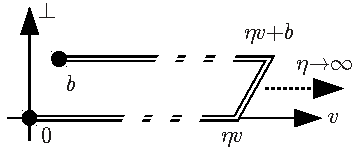
\includegraphics[width=0.5\linewidth]{figures/StapleLink2.pdf}
    \caption{Staple-shaped gauge link as in SIDIS and DY, following Ref.~\cite{Musch:2011er}.}
    \label{fig:staple}
\end{figure}

In Fig. \ref{fig:staple}, the two parallel Wilson lines are connected at the far end by another straight Wilson line. The complete gauge link thus has a staple-like shape. The vector $v$ sets the staple direction, and $\eta$ sets its extent. Lattice calculations are typically performed without any gauge fixing. We therefore prefer the notation with an explicitly gauge-invariant operator. Moreover, we compute at several finite staple extents $\eta$ (in lattice units, $\eta=0,\ldots,10$) and study the $\eta$ dependence. The $\eta\to\infty$ behavior is addressed through the fit range $6\le\eta\le10$ and the shared $\eta$ profile discussed in Sec.~\ref{sec:fit_strategy}. Even at finite $\eta$, this gauge-link geometry satisfies the desired symmetry transformation rules listed in Appendix~\ref{app:symmetries}. In this phenomenology frame, quark separation $b$ and staple extent $v$ are spacelike; in the lattice frame, however, they become purely spatial, as discussed in Sec.~\ref{sec:amplitudes_lattice}. 

The Lorentz-invariant Collins-Soper parameter, $\zeta \equiv 2 v \tcdot P/\sqrt{|v^2|}$, parameterizes the approach toward the physical light-like limit ($v = \nminus$). As $v$ becomes light-like, $\zeta \rightarrow \infty$; the parameter acts as an artificial scale that regulates the rapidity divergences~\cite{Collins:1981uk, Idilbi:2004vb, Aybat:2011ge}. Expressing the vectors $P$ and $v$ via rapidities $y_P$ and $y_v$ (we use $P^{\pm} = \mN e^{\pm y_P} / \sqrt{2}$ and $v^+/v^- = - e^{2y_v}$, with $v^->0$), we define the dimensionless variable:
\begin{equation}
	\hat \zeta \equiv \zeta / 2 \mN =  \frac{v \cdot P}{\sqrt{|v^2|} \sqrt{P^2}}=  \frac{v^+P^-+v^-P^+}{\sqrt{|v^2|} \mN} = \sinh(y_P - y_v)\ ,
	\label{eq-zeta}
\end{equation}
So $\hat \zeta$ measures the rapidity difference between the nucleon momentum and the Wilson line direction. This allows us to boost to a frame where $v$ is purely spatial ($v^0 = 0, y_v = 0$), which will be suited for lattice calculations.

\subsection{Amplitudes and the TMDs \texorpdfstring{$f_1$}{f1} and \texorpdfstring{$f_{1T}^\perp$}{f1Tperp}}
\label{sec:amplitudes_tmds}
The correlator $\widetilde\Phi^{[\gamma^\mu]}_\unsub$ is decomposed into Lorentz-invariant amplitudes $\tAmp_i$ and $\tBmp_i$, following Refs.~\cite{Musch:2011er,Goeke:2005hb}; the decomposition and the symmetry constraints on it are given in Appendix~\ref{app:symmetries}. In our frame ($b^+=0$, $\vprp{v}=\vprp{P}=0$), the kinematics fixes the relation between the invariants~\cite{MuschThesis2, Accardi:2009au}:
\begin{widetext}
\begin{align}
	\frac{v \tcdot b}{v \tcdot P} = b \tcdot P \frac{R(\zetahat^2)}{\mN^2}\, , \quad \text{where} \quad R(\zetahat^2) \equiv 1- \sqrt{1 + \hat \zeta^{-2}} = \frac{\mN^2}{v \tcdot P} \frac{v^+}{P^+} \, .
	\label{eq-lindeprel}
\end{align}
\end{widetext}
The relation in Eq. \eqref{eq-lindeprel} shows that the third argument of the $\tAmp_i$ and $\tBmp_i$ is not independent of the others in the context of TMDs.
Moreover, in our lattice calculations, we have to choose the link directions $b$ and $v$ such that Eq. \eqref{eq-lindeprel} is fulfilled. 
As a side remark, the parameter corresponding to Eq. \eqref{eq-lindeprel} in momentum space is $v \tcdot k / v \tcdot P \approx x$, i.e., the amplitudes $A_i$ and $B_i$ acquire an explicit $x$-dependence, which has already been pointed out in Refs.~\cite{MuschThesis2,Accardi:2009au}.
For the $\Gamma=\gamma^+$ structure at leading twist, the correlator can be written in the form 
\begin{align}
	\frac{1}{2 P^+}\widetilde \Phi^{[\gamma^+]}_{\unsub} & = 	
		\tAmp_{2B} 
		+ i \mN \epsilon_{ij} \vect{\bvec}_i \vect{S}_j\, \tAmp_{12B} \ ,
\end{align}
where the indices $i,j$ correspond to transverse directions, $i,j\in \{1,2\}$
(we use the convention $\epsilon^{0123}=1$ for the totally antisymmetric Levi-Civita symbol, and introduce $\myeps_{i j} \equiv \epsilon^{-+ij}$ such that $\myeps_{1 2} = 1$), and where we
have introduced the following abbreviations for combinations of amplitudes:
\begin{align}
	\tAmp_{2B}  & \ \equiv\  \tAmp_2 + R(\zetahat^2) \tBmp_1 \nonumber \displaybreak[0] \\
	\tAmp_{12B}  & \ \equiv\  \tAmp_{12} - R(\zetahat^2) \tBmp_8 \ . \displaybreak[0] 
	\label{eq-ABamps_sivers}
\end{align}
The unpolarized distribution $f_1$ and the Sivers distribution $f_{1T}^\perp$ follow from the Fourier integration operator $\fourint$:
\begin{widetext}
\begin{align}
	\fourint \tAmp_i \equiv & \int \frac{d^2 \vprp{\bvec}}{(2\pi)^2}\,e^{-i\vprp{\bvec}\tcdot\vprp{\kei}}\, \frac{1}{\widetilde{\mathcal{S}}(\bvec^2;\ldots)} \int \frac{d(\bvec \tcdot P)}{(2\pi)}\,e^{ix(\bvec \tcdot P)} 
	\tAmp_i(-\vprp{\bvec}^2,\bvec \tcdot P,(\bvec \tcdot P) R(\zetahat^2)/\mN^2,-1/(\mN\zetahat)^2,\eta v \tcdot P) \nonumber \\
	= & \int_0^\infty \frac{d(-\bvec^2)}{2(2\pi)}\ \frac{J_0(\sqrt{-\bvec^2}\, |\vprp{\kei}|)}{\widetilde{\mathcal{S}}(\bvec^2;\ldots)}\ \int \frac{d(\bvec \tcdot P)}{(2\pi)}\,e^{ix(\bvec \tcdot P)}\ 
	\tAmp_i(\bvec^2,\bvec \tcdot P,(\bvec \tcdot P) R(\zetahat^2)/\mN^2,-1/(\mN\zetahat)^2,\eta v \tcdot P) \, 
	\label{eq-fourint}
\end{align}
\end{widetext}
Applied to the combined amplitudes, it gives the leading-twist distributions:
\begin{align}
	 f_1(x,\vprp{\kei}^2;\zetahat,\ldots,\eta v \tcdot P) & = 2 \fourint\ \tAmp_{2B} \,,\nonumber \displaybreak[0] \\
	 f_{1T}^\perp(x,\vprp{\kei}^2;\zetahat,\ldots,\eta v \tcdot P) & =  4 m_N^2 \partial_{\vprp{\kei}^2} \fourint\ \tAmp_{12B} \ .
	 \label{eq-tmdsfromampsodd}
\end{align} 
Here, the dots ``$\ldots$'' indicate further parameters that specify the geometry of the soft factor. 
The $f_1$ is a T-even distribution which fulfills
\begin{align}
	f^{\text{T-even}}(x,\vprp{\kei}^2;\zetahat,\ldots,\eta v \tcdot P) = f^{\text{T-even}}(x,\vprp{\kei}^2;\zetahat,\ldots,-\eta v \tcdot P)
\end{align}
while the Sivers function $f_{1T}^\perp$ is a T-odd distribution which fulfills
\begin{align}
	f^{\text{T-odd}}(x,\vprp{\kei}^2;\zetahat,\ldots,\eta v \tcdot P) & = - f^{\text{T-odd}}(x,\vprp{\kei}^2;\zetahat,\ldots,-\eta v \tcdot P)
\end{align}
As a result, T-odd distributions must vanish for $\eta = 0$, which corresponds to straight gauge links.
TMDs for SIDIS and DY are obtained for $\eta v \tcdot P \rightarrow \infty$ and $\eta v \tcdot P \rightarrow -\infty$, respectively.
In the following, we choose $v \tcdot P \geq 0$, such that the SIDIS and DY limits for space-like $v$ can also be written as $\eta |v| \rightarrow \infty$ and $\eta |v| \rightarrow -\infty$, respectively.


Equation~\eqref{eq-tmdsfromampsodd} shows that the $x$-dependent TMDs in Fourier space, $\tilde f(x,\vprp{\bvec}^2)$ as defined in Eqs.~\eqref{eq-FTMD} and \eqref{eq-dFTMD}, are given directly by the Fourier transform of the amplitudes $\tAmp_{iB}$ with respect to $\bvec \tcdot P$.
For brevity, define the $x-(\bvec\tcdot P)$-Fourier-transformed, soft-factor-divided amplitudes
\begin{widetext}
\begin{equation}
	\tAmp^{[x]}_i(x,\vprp{\bvec}^2) \equiv \frac{1}{\widetilde{\mathcal{S}}(-\vprp{\bvec}^2;\ldots)} \int_{-\infty}^{\infty} \frac{d(\bvec \tcdot P)}{2\pi}\, e^{ix(\bvec \tcdot P)}\, \tAmp_{i}\big(-\vprp{\bvec}^2,\bvec \tcdot P,\ldots\big)\,,
\end{equation}
\end{widetext}
\begin{widetext}
\begin{align}
	\tilde f_1^{(0)}(x, \vprp{\bvec}^2;\zetahat,\ldots,\eta v \tcdot P) & = 2 \int_{-\infty}^{\infty} \frac{d(\bvec \tcdot P)}{2\pi}\, e^{ix(\bvec \tcdot P)}\, 
	\frac{\tAmp_{2B}\big(-\vprp{\bvec}^2,\bvec \tcdot P,(\bvec \tcdot P) R(\zetahat^2)/\mN^2,-1/(\mN\zetahat)^2,\eta v\tcdot P\big)}{\widetilde{\mathcal{S}}(-\vprp{\bvec}^2;\ldots)} \,,\displaybreak[0] \nonumber \\
    &=2\, \tAmp^{[x]}_{2B}(x,\vprp{\bvec}^2)\,. \label{eq-xintderfttmds1}\\
	\tilde f_{1T}^{\perp(1)}(x, \vprp{\bvec}^2;\zetahat,\ldots,\eta v \tcdot P) & = -2 \int_{-\infty}^{\infty} \frac{d(\bvec \tcdot P)}{2\pi}\, e^{ix(\bvec \tcdot P)}\, 
	\frac{\tAmp_{12B}\big(-\vprp{\bvec}^2,\bvec \tcdot P,(\bvec \tcdot P) R(\zetahat^2)/\mN^2,-1/(\mN\zetahat)^2,\eta v\tcdot P\big)}{\widetilde{\mathcal{S}}(-\vprp{\bvec}^2;\ldots)} \, ,\nonumber \\
    &=-2\,\tAmp^{[x]}_{12B}(x,\vprp{\bvec}^2)\,.
	\label{eq-xintderfttmds2}
\end{align}
\end{widetext}
We drop the soft-factor term from the definitions below, since it cancels in the ratios we consider.

\subsection{Generalized Sivers shift}
\label{sec:sivers_shift_amplitudes}
The derivation of Eqs.~\eqref{eq-xintderfttmds1} and~\eqref{eq-xintderfttmds2} is in Appendix~\ref{app:symmetries}; the arguments of the amplitudes are defined in Eq.~\eqref{eq-ab} there. Eqs. \eqref{eq-xintderfttmds1}-\eqref{eq-xintderfttmds2} identify $x$-dependent derivatives of Fourier-transformed TMDs with simple linear combinations of amplitudes $\tAmp_i$ and $\tBmp_i$ evaluated at the same values of $\vprp{\bvec}^2$, $\bvec \cdot P$, $\zetahat$ and $\eta v \tcdot P$. Forming ratios of these objects thus amounts to taking ratios of linear combinations of the fundamental correlators $\tilde \Phi^{[\Gamma]}_\unsub$ evaluated at the same point, i.e., with the same values of $\bvec$, $P$, and $\eta v$. For a discussion of the renormalization properties of ratios of the objects in \eqref{eq-xintderfttmds1}-\eqref{eq-xintderfttmds2}, it is thus sufficient to understand the renormalization properties of (ratios formed from) the correlators $\widetilde \Phi^{[\Gamma]}_\unsub = \frac{1}{2} \, \bra{P, S}\ \bar{q}(0)\, \Gamma\ \mathcal{U}\ q(\bvec)\ \ket{P, S} $.

As discussed in Refs.~\cite{Musch:2011er, Yoon:2017qzo}, analytical studies of the operator $\bar{q}(0)\, \Gamma\, \mathcal{U} q(\bvec)$ in the continuum suggest that for $\bvec^2 \neq 0$ the renormalization factors are multiplicative and $\Gamma$-independent. We will assume here that our lattice representation of $\bar{q}(0)\, \Gamma\, \mathcal{U}\, q(\bvec)$ is renormalized multiplicatively independent of $\Gamma$ as long as $|b|$ is larger than a few lattice spacings. In the fits of Sec.~\ref{sec:results} we use $|b|\ge 3a$ (Sec.~\ref{sec:fit_strategy}). A more detailed discussion and numerical studies of this operator's renormalization properties appear in Ref.~\cite{Musch:2010ka}. Under the assumption of multiplicative renormalization, the soft factor and the renormalization factors cancel in ratios of amplitudes evaluated at the same $\bvec$, $P$ and $\eta v$, and such ratios depend only on $\vprp{\bvec}^2$, $P\cdot b$, $\zetahat$, and the staple extent $\eta v \tcdot P$.

From phenomenology, the Sivers shift is the ratio defined as
\begin{widetext}
\begin{align}
	\langle \vect{k}_y \rangle_{TU} \equiv \mN \frac{f_{1T}^{\perp(1)}(x)}{f_1^{(0)}(x)} = 
	\left. \frac{ \int d^2 \vprp{\kei}\, \vect{\kei}_y  \ \Phi^{[\gamma^+]}(x,\vprp{\kei},P,S;\ldots) }{ \int d^2 \vprp{\kei}  \phantom{\vect{\kei}_y}\ \Phi^{[\gamma^+]}(x,\vprp{\kei},P,S;\ldots) } \right|_{\displaystyle \vprp{S}=(1,0) }\, , \label{eq-sivshift}
\end{align}
\end{widetext}
where $\gamma^+$ projects onto the leading twist.
The ratio above yields the average transverse momentum
in the $y$-direction, for quarks with a given longitudinal momentum fraction $x$ inside a proton polarized in the $x$-direction. As mentioned before, understanding $f_{1T}^{\perp(1)}$ simply as a $\vprp{\kei}$-weighted TMD is problematic, since the $\vprp{k}$-integral is expected to be UV divergent. 
A natural way of circumventing this divergence is to generalize the Sivers shift to an expression in terms of the Fourier-transformed TMDs:
\begin{widetext}
\begin{align}
    \langle \vect{k}_y \rangle_{TU}(\vprp{\bvec}^2,x,\zetahat,\eta v \tcdot P) 
	&\ \equiv\ \mN \frac{\tilde f_{1T}^{\perp(1)}(\vprp{\bvec}^2,x;\zetahat,\ldots,\eta v \tcdot P)}{\tilde f_1^{(0)}(\vprp{\bvec}^2,x;\zetahat,\ldots,\eta v \tcdot P)}  \\
 &=-m_{N} \frac{\int d(b\cdot P)e^{ix(b\cdot P)} \tAmp_{12B}(\bvec^2,\bvec \tcdot P,(\bvec \tcdot P) R(\zetahat^2)/\mN^2,-1/(\mN\zetahat)^2,\eta v \tcdot P)}{\int d(b\cdot P)e^{ix(b\cdot P)}\tAmp_{2B}(\bvec^2,\bvec \tcdot P,(\bvec \tcdot P) R(\zetahat^2)/\mN^2,-1/(\mN\zetahat)^2,\eta v \tcdot P)} \\
 &\ \xrightarrow{\vprp{\bvec}^2 = 0} 
		\left. \frac{  \int d^2 \vprp{\kei}\, \vect{\kei}_y  \ \Phi^{[\gamma^+]}(x,\vprp{\kei},P,S;\ldots) }
		{  \int d^2 \vprp{\kei}  \phantom{\vect{\kei}_y}\ \Phi^{[\gamma^+]}(x,\vprp{\kei},P,S;\ldots) } \right|_{\displaystyle \vprp{S}=(1,0) } 
	\label{eq-genSivShift}
\end{align}
\end{widetext}
In the limit $\vprp{\bvec}^2=0$ we recover the Sivers shift \eqref{eq-sivshift}, because the Fourier transformed TMDs $\tilde f_{1T}^{\perp(1)}$ and $\tilde f_1^{(0)}$ coincide with the moments $f_{1T}^{\perp(1)}$ and $f_1^{(0)}$, respectively. However, we are interested in the generalized Sivers shift for non-zero $\vprp{\bvec}^2$, where this UV divergence disappears. The variable $\vprp{b}^2$ effectively acts as a regulator. Moreover, the $\vprp{\bvec}$-dependence allows us to study differences in the widths of distributions on a qualitative level.

Furthermore, the generalized Sivers shift is T-odd, i.e., we expect to obtain results of opposite sign in the SIDIS and DY limits $\eta v \tcdot P \rightarrow \infty$ and $\eta v \tcdot P \rightarrow -\infty$, respectively, as demonstrated in Refs.~\cite{Musch:2011er,Yoon:2017qzo}.

In summary, the generalized Sivers shift describes a feature of the transverse momentum distribution of (unpolarized) quarks in a transversely polarized proton. In the formal limit $\vprp{\bvec}^2 = 0$, it measures the dipole moment of that distribution orthogonal to the polarization of the proton.


\section{Amplitudes from Lattice Data}
\label{sec:amplitudes_lattice}

Because $x$ and the longitudinal spatial separation $b \cdot P$ are Fourier conjugate variables, mapping the $x$-dependence requires a Fourier transform of these amplitudes with respect to $b \cdot P$. Analytically, the $x$-dependent Sivers shift takes the form:
\begin{align}
	&\langle \vect{k}_y \rangle_{TU}(\vprp{\bvec}^2,x,\zetahat,\eta v \tcdot P)
	\equiv \mN \frac{\tilde f_{1T}^{\perp(1)}}{\tilde f_1^{(0)}} \nonumber \\
	&\quad = -\mN \frac{\int d(\bvec\tcdot P)\,e^{ix(\bvec\tcdot P)}\, \tAmp_{12B}(\cdots)}{\int d(\bvec\tcdot P)\,e^{ix(\bvec\tcdot P)}\,\tAmp_{2B}(\cdots)} \nonumber \\
	&\quad = -\mN \frac{\tAmp_{12B}^{[x]\text{Re}}(\cdots)-\tAmp_{12B}^{[x]\text{Im}}(\cdots)}{\tAmp_{2B}^{[x]\text{Re}}(\cdots)-\tAmp_{2B}^{[x]\text{Im}}(\cdots)}\ .
	\label{eq:sivers_shift_xdep}
\end{align}
 Expanding the Fourier phase factor into its trigonometric components isolates the real and imaginary contributions of the amplitudes to the Sivers shift. Because the integration over $d(b \cdot P)$ is performed over a symmetric domain, the non-vanishing terms of the integral are dictated by the parity of the integrands with respect to $b \cdot P$. The trigonometric weights $\cos\left(x(b\cdot P)\right)$ and $\sin\left(x(b\cdot P)\right)$ are even and odd, respectively.

This harmonic symmetry filters the invariant amplitudes based on their behavior under Hermitian conjugation. By Eqs.~\eqref{conditi_hermitian} and~\eqref{eq-ReIm-parity}, the real components $\tAmp_{2B}^{\text{Re}}$ and $\tAmp_{12B}^{\text{Re}}$ are even functions of $b \cdot P$, while the imaginary components $\tAmp_{2B}^{\text{Im}}$ and $\tAmp_{12B}^{\text{Im}}$ are odd. (Parity in $b$ is parity in $b\cdot P$ here, because $\bvec^2$ is unchanged under $b\to-b$, $v\cdot b$ is tied to $b\cdot P$ by Eq.~\eqref{eq-lindeprel}, and $R(\zetahat^2)$ is real.) Only the symmetric products therefore survive the integration, i.e., the even real amplitudes coupled with the cosine term and the odd imaginary amplitudes coupled with the sine term. Here, $\tAmp_{iB}^{[x]\text{Re}}$ and $\tAmp_{iB}^{[x]\text{Im}}$ are the Fourier-transformed amplitudes. Note that, since $\tAmp_{iB}^{\text{Im}}$ is odd in $(P\cdot b)$, its Fourier transform gives an imaginary solution, i. e. $\int \frac{d(\bvec \tcdot P)}{2\pi}e^{ix(b\cdot P)}\tAmp_{iB}^{\text{Im}}=i\tAmp_{iB}^{[x]\text{Im}}$, this results in
\begin{align}
    \int \frac{d(\bvec \tcdot P)}{2\pi}e^{ix(b\cdot P)} \left[\tAmp_{iB}^{\text{Re}}+i\tAmp_{iB}^{\text{Im}}\right]=&\left[\tAmp_{iB}^{[x]\text{Re}}+i^2\tAmp_{iB}^{[x]\text{Im}}\right]\\
    =&\left[\tAmp_{iB}^{[x]\text{Re}}-\tAmp_{iB}^{[x]\text{Im}}\right]
    \label{reminusimag-amp}
\end{align}
for both unpolarized and Sivers TMD amplitudes. 

The parity components are extracted from the lattice data as described below.


For the Collins-Soper parameter $\hat{\zeta}$ of Eq.~\eqref{eq-zeta}, the staple direction $v$ on the lattice must be space-like ($v^2 < 0$), so the physical TMD limit is recovered only by extrapolating $\hat{\zeta} \to \infty$. In practice, since $v$ is a purely spatial vector on the lattice ($v_0 = 0$), increasing $\hat{\zeta}$ requires simulating the nucleon at progressively higher spatial momenta $\vect{P}$. Tracking the evolution of the Sivers shift across multiple $\hat{\zeta}$ values is therefore necessary for phenomenological predictions.

We now move to the frame in which the lattice calculation is performed. To perform the Fourier transform over $b \cdot P$, we require a lattice geometry with both non-zero $b \cdot P$ and zero $b \cdot P$. However, the Lorentz-invariant arguments of the amplitudes are not independent. The phenomenological frame ($b^+=0, \vprp{P}=0$) enforces the constraint of Eq.~\eqref{eq-lindeprel}. Expanding the dot products in the case where the momentum is directed along the 1-axis ($P = (E, P_1, 0, 0)$), we find:
\begin{align}
    b_{1}|v|\left[\frac{P_{1}}{m_{N}}\left(\hat{\zeta}-\sqrt{\hat{\zeta}^2+1}\right)+\hat{\zeta}\frac{m_{N}}{P_{1}}\right]=\vec{v}_{T}\cdot\vec{b}_{T} \ .\label{constraints}
\end{align}
To satisfy this equation over a continuous range of $b \cdot P$ without coupling the transverse separation $\vec{b}_T$ directly to the longitudinal staple geometry, we orient the transverse separation vectors orthogonally. By choosing $\vec{v}_{T}=(0,v_{3})$ and $\vec{b}_{T}=(b_{2},0)$, the right-hand side identically vanishes ($\vec{v}_{T}\cdot\vec{b}_{T} = 0$). This is not the only choice, but it is convenient for a lattice calculation because both $b$ and $v$ can remain in 2-dimensional lattice planes. In general, $b$ and $v$ may have to point in arbitrary directions in three-dimensional space.

For a given lattice momentum, setting the bracket to zero fixes $\hat\zeta$ and the staple direction; the explicit calculation for the lowest momentum $P_1=-1$ is in Appendix~\ref{app:explicit_zeta}. The results for all four momenta are collected in Table~\ref{tab:zeta_directions}.


This geometric calculation is repeated over a range of nucleon momenta to increase $\hat{\zeta}$ systematically. The resulting constraint parameters are summarized in Table \ref{tab:zeta_directions}.

\begin{table}[htbp]
    \centering
    \renewcommand{\arraystretch}{1.3}
    \begin{tabular}{|c|c|c|}
    \hline
        $\vect{P}\cdot a\hat{L}/(2\pi)$ & $\hat{\zeta}$ &  $v_{1}$\\
        \hline
        $(-1,0,0)$ & $\pm 0.090772$ &$v_{1}=\pm 0.301~v_{3}$\\
        \hline
        $(-2,0,0)$ & $\pm 0.294367$ &$v_{1}=\pm 0.531~v_{3}$\\
        \hline
        $(-3,0,0)$ & $\pm 0.539684$ &$v_{1}=\pm 0.689~v_{3}$\\
        \hline
        $(-4,0,0)$ & $\pm 0.785756$ &$v_{1}=\pm 0.786~v_{3}$\\
        \hline
    \end{tabular}
    \caption{Resulting Collins-Soper parameters ($\hat{\zeta}$) and the necessary geometric constraint on the staple vector components to ensure the full $b \cdot P$ range is scanned.}
    \label{tab:zeta_directions}
\end{table}

\begin{table}[htbp]
    \centering
    \renewcommand{\arraystretch}{1.3}
    \resizebox{\columnwidth}{!}{\begin{tabular}{|c|c|c|}
    \hline
       $\vect{\bvec}/a$  &  $\eta \vect{v}/a$ & $\vect{P}\cdot a\hat{L}/(2\pi)$\\
       \hline
        $(b_{1},b_{2},0)$ & $ \eta\cdot(v_{1},0,v_{3})$, $\eta=0,\cdots,10$  & $(n,0,0)$, $n=-1,-2,-3,-4$\\
        \hline
    \end{tabular}}
    \caption{Configuration parameters for the Lattice QCD non-local matrix element extraction. Our lattice size is $\{\hat{L}^3\times\hat{T}\}=\{32^3\times96\}$ and the lattice spacing is $a=0.11403\text{ fm}$.}
    \label{tab:lattice_params}
\end{table}
A consequence of Table \ref{tab:zeta_directions} is that the staple vector $v$ cannot align cleanly with the Cartesian axes of the Euclidean grid. Instead, it must point in an off-axis direction within the $v_1-v_3$ plane. For example, to achieve $v_1 = 0.301~v_3$ at $|P| = 1$, the Wilson line must trace an oblique, step-wise path across the discrete lattice sites (e.g., traversing roughly three lattice spacings in the 1-direction for every ten in the 3-direction). Figure \ref{fig:v_allzetahat} plots the resulting staple directions in the $v_1-v_3$ plane for all four Collins-Soper values in Table \ref{tab:zeta_directions}.

\begin{figure}[htpb]
    \centering
    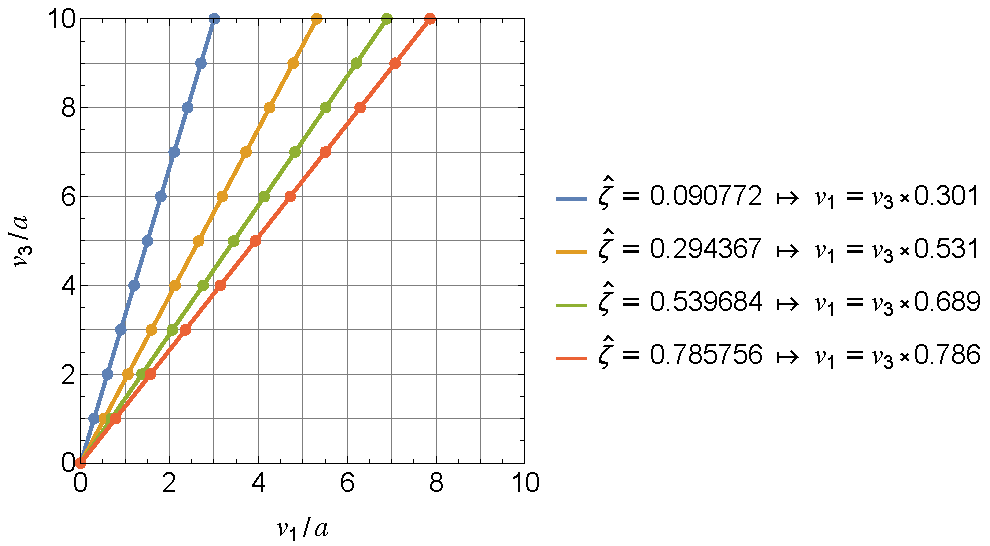
\includegraphics[width=\linewidth]{figures/v1_v2_allzetahat_plot.pdf}
    \caption{Directions of the spatial staple vectors $\vect{v}$ mapped in the $v_1-v_3$ plane. Each vector corresponds to the requisite geometry to satisfy the $b \cdot P \neq 0$ constraint for the four sequential Collins-Soper parameters $\hat{\zeta}$.}
    \label{fig:v_allzetahat}
\end{figure}

To evaluate the correlation function as a function of the staple extent, we scale the direction vector $\vect{v}$ by an increment $\eta$, and $\vect{v}$ is a unit vector. The physical length of the staple is thus governed by the coordinate $\eta \vect{v}/a$. Because $\vect{v}$ points in a continuous, off-axis direction, scaling it by integer values of $\eta$ generally yields target coordinates that fall somewhere between the discrete Cartesian lattice sites. 

 To access the continuous off-axis coordinate $\eta \vect{v}/a$, we employ a spatial bounding and interpolation strategy. Rather than constructing a single, potentially biased step-wise path (a ``staircase'') that roughly approximates the vector, we compute the observable at multiple distinct integer lattice sites surrounding the exact ideal target coordinate. We reach these bounding coordinates through specific permutations of unit links. A path sequence denoted $\{1,3,1\}$ is a single link in the $\hat{x_{1}}$ direction, followed by one in the $\hat{x_{3}}$ direction and a final link in the $\hat{x_{1}}$ direction, which lands at the integer coordinate $(2,0,1)$. By varying these step sequences, we gather data at three to four adjacent lattice sites (e.g., on either side of the target along the $x^3$ slice). 

Once these bounding matrix elements are computed, we perform a spatial interpolation inside the Jackknife resampling loop to extract the value at the continuous target coordinate $\eta \vect{v}/a$. The interpolation reduces discretization artifacts and the staircase errors of off-axis Wilson lines; the procedure is described below. Figures \ref{fig:v_path_P-1}--\ref{fig:v_path_P-4} and Tables \ref{tab:eta_table_P-1}--\ref{tab:eta_table_P-4} of Appendix~\ref{app:paths} show the ideal continuous trajectories for each nucleon momentum, together with the corresponding discrete bounding paths and link sequences.
Before interpolating to the off-axis target $\eta \vect{v}/a$, we must account for path degeneracy. Because the lattice gauge links are restricted to the Cartesian axes, there are multiple step-wise permutations (different side-link paths) that terminate at the same physical lattice coordinate. While these paths are geometrically equivalent at their endpoints, they are different lattice operators with the same continuum limit and can have distinct discretization artifacts and gauge noise. As illustrated in Figure \ref{fig:example_2path}, to improve the symmetry, we average the correlation functions evaluated over all degenerate paths that share the same endpoint. Path averaging symmetry-improves the lattice operators and reduces the gauge noise before any interpolation. % TODO(Hari): quantify the noise reduction; state that the same path set is used for every $\Gamma$

\begin{figure}[htpb]
    \centering
    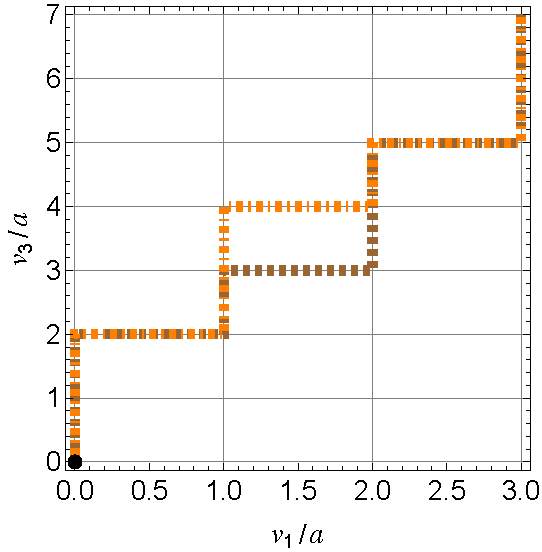
\includegraphics[width=0.5\linewidth]{figures/Example_v_plot_with_2path.pdf}
    \caption{Illustration of path degeneracy. Two distinct step-wise gauge link permutations (e.g., solid and dashed lines) terminate at the identical discrete lattice coordinate. We average the correlators from these equivalent paths to suppress local gauge noise before interpolation.}
    \label{fig:example_2path}
\end{figure}

Once we obtain the symmetry-improved (path-averaged) correlators at the discrete bounding sites, we perform a 1-dimensional interpolation. For a fixed transverse staple extent $v_3$, the kinematic constraint dictates an ideal continuous longitudinal component, $v_1^{\text{constraint}}$. The surrounding discrete lattice sites provide correlators at actual simulated coordinates, $v_1^{\text{lattice}}$. We define the fractional deviation from the ideal path as:
\begin{equation}
    \Delta v_1 = \frac{v_1^{\text{constraint}} - v_1^{\text{lattice}}}{a} \ .
\end{equation}
By calculating the observable at three or more bounding lattice sites, we generate a set of data points as a function of this deviation $\Delta v_1$. Within each Jackknife resampling bin (to preserve the covariance and statistical error), we perform a quadratic interpolation over these points. We then extract the physical amplitude on the continuous constraint trajectory by evaluating the interpolating polynomial exactly at $\Delta v_1 = 0$. 


A representative example of this interpolation procedure is shown in Figure \ref{fig:interpolation_ex} for a specific staple extent ($\eta=7$) and nucleon momentum ($P_1 = -1$). The red data points represent the path-averaged lattice evaluations at the discrete bounding sites, plotted against their deviation from the ideal trajectory. The solid gray curve denotes the quadratic interpolation, and the blue point highlights the final extracted physical value at $\Delta v_1 = 0$. We apply this procedure to all Dirac structures ($\Gamma$), separately for the real ($b\cdot P$-even) and imaginary ($b\cdot P$-odd) parts of the amplitudes.

\begin{figure}[htpb]
    \centering
    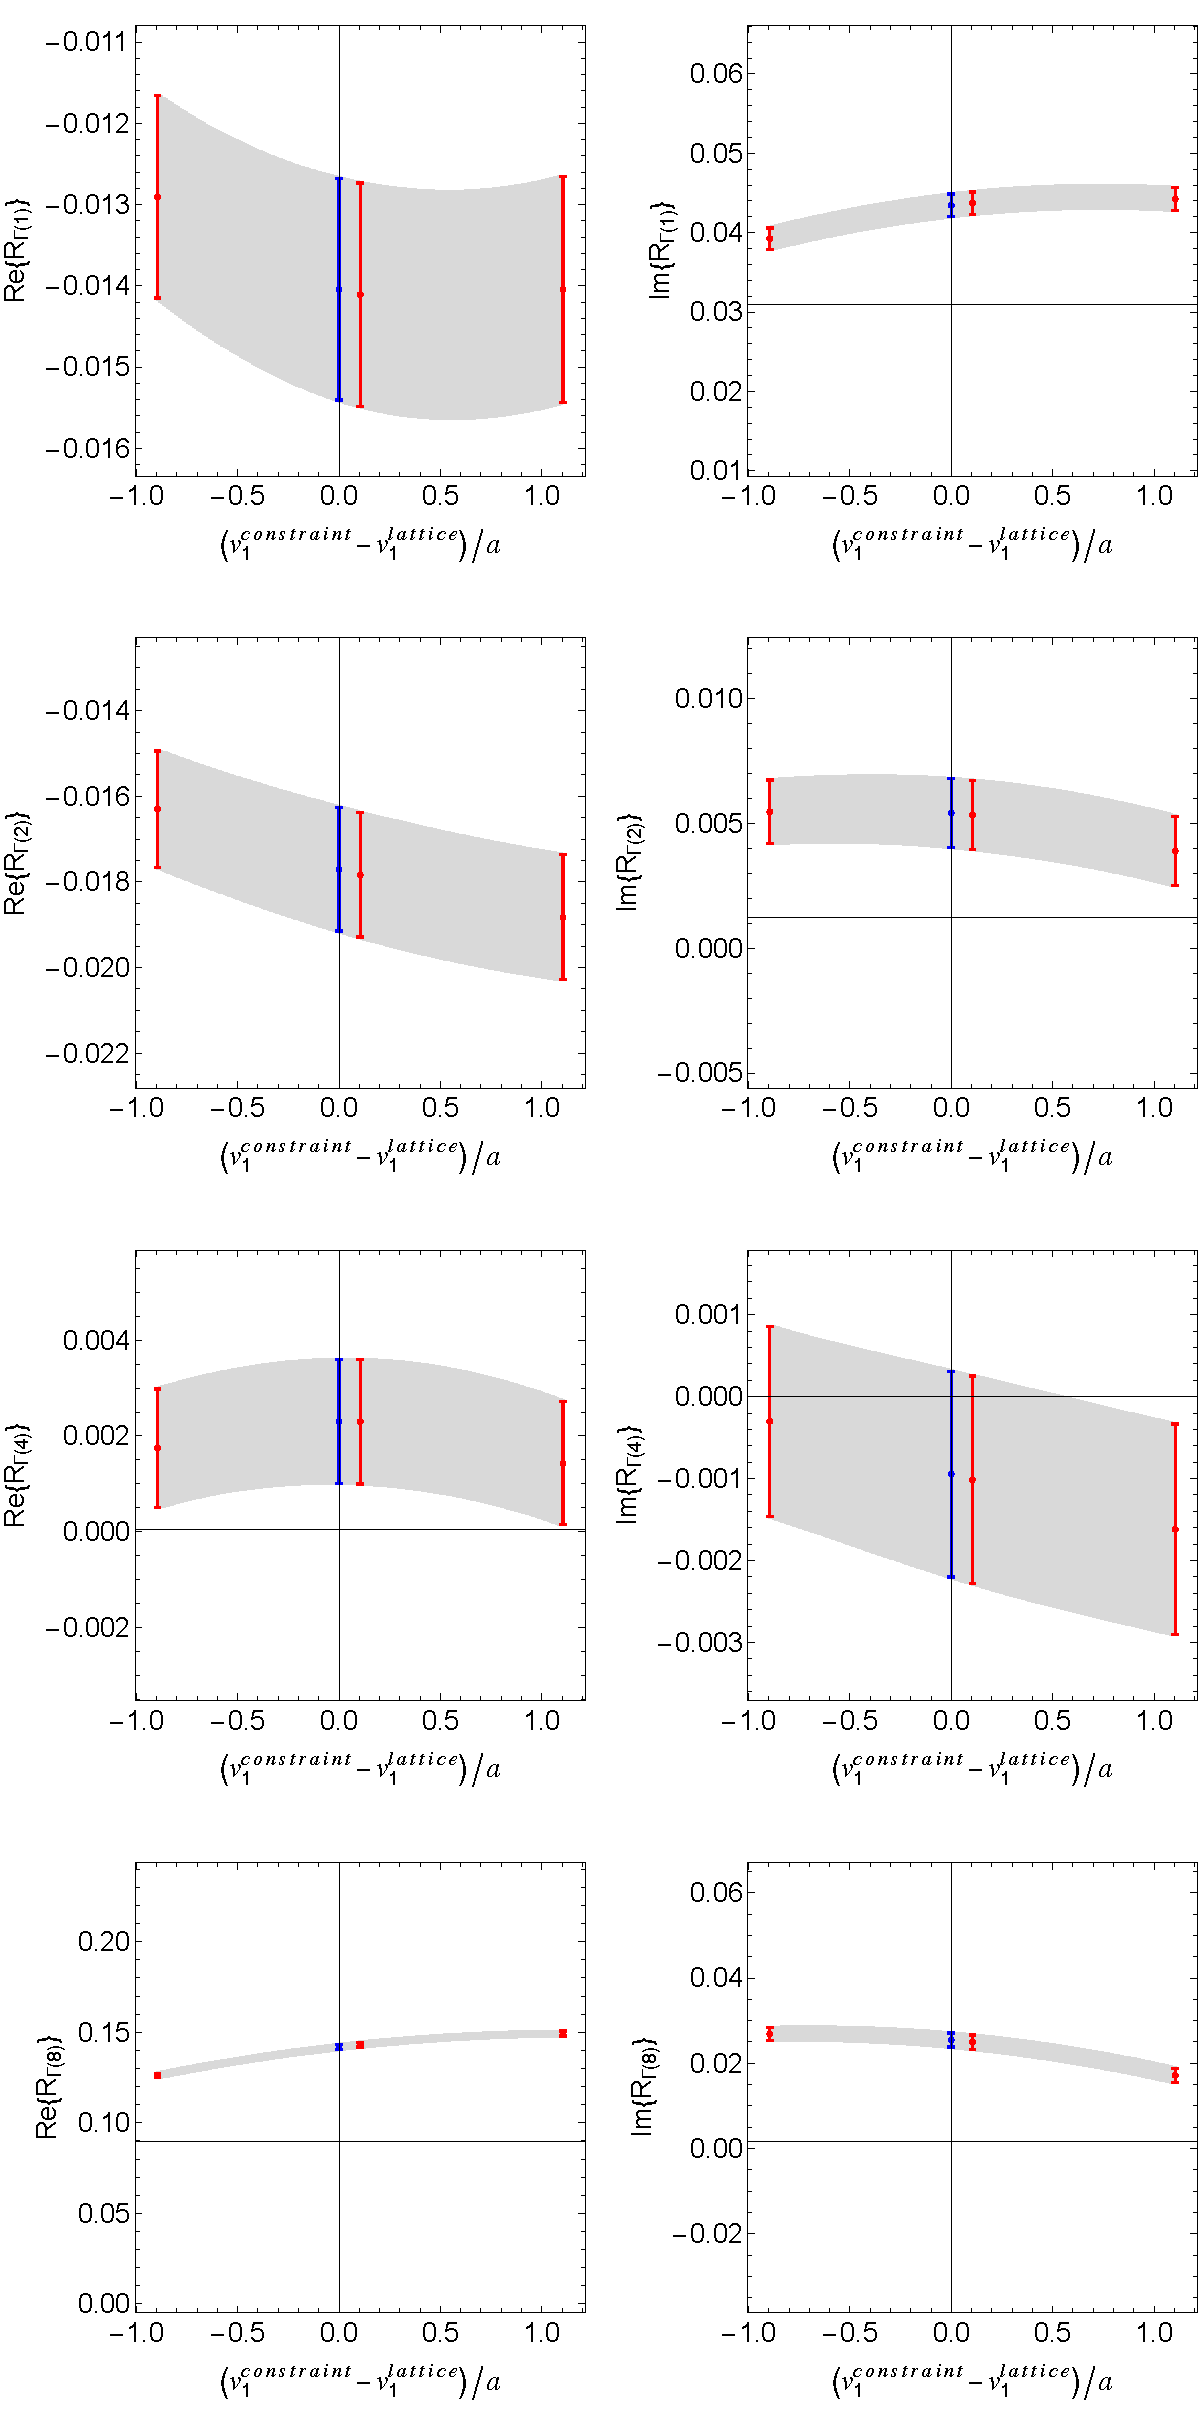
\includegraphics[width=\linewidth,height=0.65\textheight,keepaspectratio]{figures/Interpolation_Ex_b120_eta7_P-1.pdf}
    \caption{Quadratic interpolation of the real and imaginary parts of the correlation function for $\vect{b}=\{1,2,0\}$, $\eta=7$, and $\vect{P}\cdot a\hat{L}/(2\pi)=(-1,0,0)$. Red markers indicate the path-averaged lattice data points as a function of their deviation from the ideal constraint trajectory, $\Delta v_1 = (v_1^{\text{constraint}} - v_1^{\text{lattice}})/a$. The gray curve indicates the quadratic interpolant, and the central blue marker represents the final extracted value at $\Delta v_1 = 0$, lying exactly on the required off-axis spatial trajectory.}
    \label{fig:interpolation_ex}
\end{figure}

In addition to the staple vector $\vect{v}$, the correlation function depends on the spatial separation $\vect{b}$ between the initial and final quark fields. Recall that the real and imaginary parts of the invariant amplitudes ($\tAmp_{iB}^{\text{Re}}$ and $\tAmp_{iB}^{\text{Im}}$) are even and odd functions of the invariant dot product $b \cdot P$, respectively. 

Because the nucleon momentum in our lattice setup is fixed along the $\hat{x_{1}}$-axis ($P = P_1 \hat{x_{1}}$), the longitudinal separation is directly proportional to the $\hat{x_{1}}$-component of the separation vector: $b \cdot P = -P_1 b_1$. Therefore, to isolate the real and imaginary parts of the amplitudes, we must evaluate the correlator at both positive and negative values of $b_1$. By taking the symmetric (even) and antisymmetric (odd) linear combinations of the correlators evaluated at $+b_1$ and $-b_1$, we project out the real and imaginary amplitudes required for the $x$-dependent Fourier transform. The numerical Fourier transform over $b \cdot P$ requires a wide and dense grid of the separation vector $\vect{b}$. Figures \ref{fig:bL_bT_path}-\ref{fig:bL_bT_standard} show the parameter space of our calculations. The left panel shows the discrete Cartesian grid in the $b_1-b_2$ plane. The right panel shows how this grid maps onto the phenomenologically relevant invariant Variable Space spanned by $(b \cdot P)\hat{L}/(2\pi)$ and the absolute separation $|b|/a$; the mapping shifts with the target Collins-Soper parameter $\hat{\zeta}$. Where, $\hat{L}$ is the spatial lattice length $\hat{L}=32$, and $a=0.11403\text{ fm}$ is the lattice spacing. 

\begin{figure}[htpb]
    \centering
    \begin{minipage}{0.35\textwidth}
        \centering
        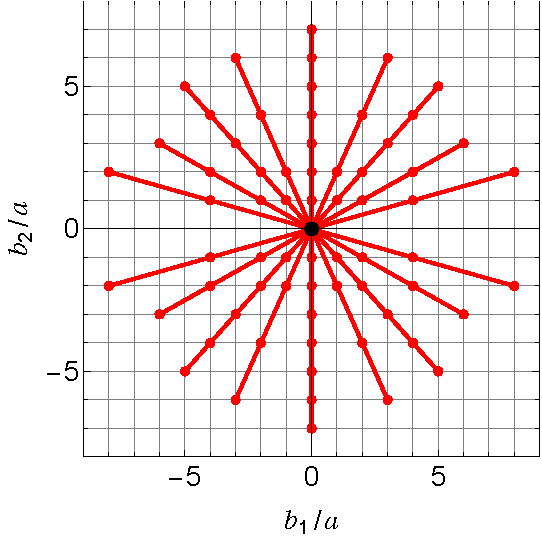
\includegraphics[width=\linewidth]{figures/bL_bT_plot.pdf}
        \caption{The sampled operator separation vectors mapped in the spatial $b_1-b_2$ plane (where $b_1 \equiv b_L$ and $b_2 \equiv b_T$).}
        \label{fig:bL_bT_path}
    \end{minipage}
    \hspace{0.05\textwidth} % Adds a controlled gap between the two smaller images
    \begin{minipage}{0.45\textwidth}
        \centering
        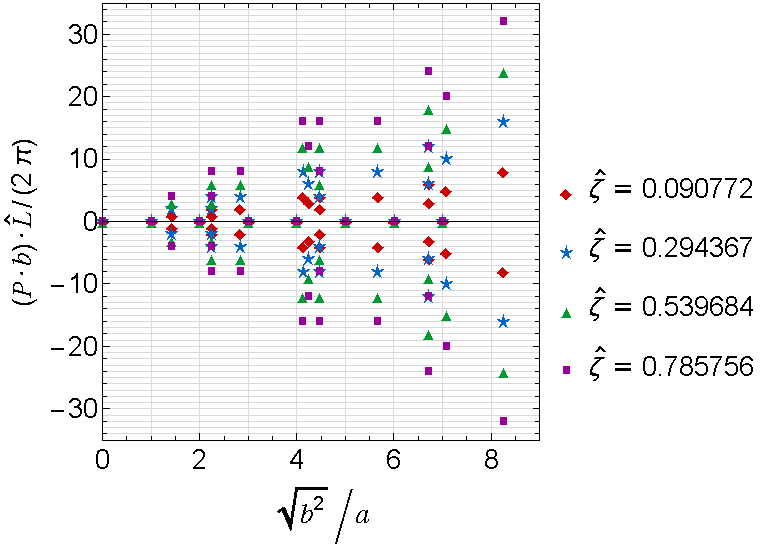
\includegraphics[width=\linewidth]{figures/Pb_bsq_plot.pdf}
        \caption{Mapping of the spatial lattice vectors into the physical invariant Variable Space $(b \cdot P/(2\pi), |b|/a)$. The trajectories diverge based on the selected target $\hat{\zeta}$.}
        \label{fig:bL_bT_standard}
    \end{minipage}
\end{figure}
The gauge-link paths used to reach each $\vect{b}$ and their path averaging are listed in Appendix~\ref{app:paths}.

We contract the amplitude decomposition of Eq.~\eqref{eq-phitildedecomp} with the lattice kinematics $P^\mu=(E_N,-|\vec P^1|,0,0)$, $b^\mu=(0,b_1,b_2,0)$, $v^\mu=\pm n^\prime(0,v_1,0,v_3)$ and $S^\mu=(0,0,0,1)$ for each of $\gamma^0,\ldots,\gamma^3$. Throughout this derivation, $\bvec^1$ and $\bvec^2$ denote the contravariant components of $\bvec$, so that $\bvec^1=b_L$ and $\bvec^2=b_T$ in this frame. The invariant dot product is $\bvec\cdot\bvec$; it is the quantity written $\bvec^2$ in the arguments of the amplitudes $\tAmp_i(\bvec^2,\ldots)$ and is never a component. $R_{\Gamma}$ denotes the lattice ratio observable associated with the Dirac structure $\Gamma$, normalized so that $\widetilde\Phi^{[\Gamma]}_\unsub=E_N R_\Gamma$. Here $R_\Gamma$ is the plateau of the ratio of the staple-link three-point function to the nucleon two-point function at equal source and sink momentum, as in Refs.~\cite{MuschThesis2,Musch:2011er}; the inputs are $R_{\gamma^0},\ldots,R_{\gamma^3}$.
The index $i\in\{1,2,4,8\}$ in $R_{\Gamma(i)}$ labels the Dirac structure by the bit-encoded convention $\Gamma(n)=\gamma_1^{n_0}\gamma_2^{n_1}\gamma_3^{n_2}\gamma_4^{n_3}$, with $\Gamma(1)=[+i\gamma^1]$, $\Gamma(2)=[-i\gamma^2]$, $\Gamma(4)=[+i\gamma^3]$ and $\Gamma(8)=[\gamma^0]$. Taking the symmetric and antisymmetric combinations of the data at $+b^1$ and $-b^1$ projects out the $b^1$-even (real) and $b^1$-odd (imaginary) amplitudes. The full algebra is in Appendix~\ref{app:solve}. The results are
Recalling that $v \tcdot P = v_1 P^1 = v^1 |P^1|$ in our chosen frame, each amplitude structure has its own conversion factor. Applying this mapping to the real components yields the final accessible amplitudes on the lattice:
\begin{align}
    \tAmp^{\text{Re}}_2 = & \frac{1}{2}\text{Re}\{ R_{\Gamma(8)}\}^{[b^{1}\text{-even}]} \\
    \tBmp^{\text{Re}}_1 = & \frac{E_{N}|P^1|v^1}{2\mN^2 v^3} \nonumber \\
    & \qquad \times \text{Im}\{ R_{\Gamma(4)}\}^{[b^{1}\text{-even}]} \\
    \tAmp^{\text{Re}}_{12} = & \frac{-1}{2\mN \bvec^2}\Big[\text{Re}\{ R_{\Gamma(1)}\}^{[b^{1}\text{-even}]} \nonumber \\
    & \qquad +\frac{v^3}{v^1}\text{Re}\{ R_{\Gamma(4)}\}^{[b^{1}\text{-even}]}\Big] \\
    \tBmp^{\text{Re}}_8 = & \frac{-E_N|P^1|}{2\mN^3 \bvec^2}\Big[\text{Im}\{ R_{\Gamma(8)}\}^{[b^{1}\text{-even}]} \nonumber \\
    & \qquad + \frac{|\vec{P}^1|v^3}{E_N v^1}\text{Re}\{ R_{\Gamma(4)}\}^{[b^{1}\text{-even}]} \nonumber \\
    & \qquad + 2\mN \frac{|\vec{P}^1|}{E_N} \bvec^2 \tAmp^{\text{Re}}_{12}\Big]
\end{align}
Applying the same scaling factors to the imaginary counterparts provides the complementary $b$-odd contributions:
\begin{align}
    \tAmp^{\text{Im}}_2 = & \frac{1}{2}\text{Im}\{ R_{\Gamma(8)}\}^{[b^{1}\text{-odd}]} \\
    \tBmp^{\text{Im}}_1 = & \frac{-E_{N}|P^1|v^1}{2\mN^2 v^3} \nonumber \\
    & \qquad \times \text{Re}\{ R_{\Gamma(4)}\}^{[b^{1}\text{-odd}]} \\
    \tAmp^{\text{Im}}_{12} = & \frac{-1}{2\mN \bvec^2}\Big[\text{Im}\{ R_{\Gamma(1)}\}^{[b^{1}\text{-odd}]} \nonumber \\
    & \qquad +\frac{v^3}{v^1}\text{Im}\{ R_{\Gamma(4)}\}^{[b^{1}\text{-odd}]}\Big] \\
    \tBmp^{\text{Im}}_8 = & \frac{E_N|P^1|}{2\mN^3 \bvec^2}\Big[\text{Re}\{ R_{\Gamma(8)}\}^{[b^{1}\text{-odd}]} \nonumber \\
    & \qquad - \frac{|\vec{P}^1|v^3}{E_N v^1}\text{Im}\{ R_{\Gamma(4)}\}^{[b^{1}\text{-odd}]} \nonumber \\
    & \qquad - 2\mN \frac{|\vec{P}^1|}{E_N} \bvec^2 \tAmp^{\text{Im}}_{12}\Big]
\end{align}


With the invariant amplitudes isolated by parity projection, we now combine them into the amplitudes $\tAmp_{2B}$ and $\tAmp_{12B}$ of Eq.~\eqref{eq-ABamps_sivers}, with $R(\zetahat^2)$ from Eq.~\eqref{eq-lindeprel}. 
To apply these expressions in our simulated lattice geometry, we map the contravariant spatial indices to our physical grid parameters. We define the longitudinal spatial separation as $b_L \equiv b^1$ and the transverse spatial separation as $b_T \equiv b^2$.
The invariant $\bvec\cdot\bvec$ then expands to $b_L^2 + b_T^2$ and enters only through the arguments of the amplitudes, while the prefactors in the $\tAmp_{12}$ and $\tBmp_8$ expressions below depend on the component $b_T=\bvec^2$ alone. We identify the longitudinal nucleon momentum as $P_L \equiv P^1$. 

We begin with the defining linear combination for the unpolarized amplitude, $\tAmp_{2B}$. Splitting this amplitude into its real and imaginary components yields:
\begin{align}
    \tAmp_{2B}^{\text{Re}}(b_L, b_T, \hat{\zeta}) &= \tAmp_2^{\text{Re}} + R(\zetahat^2) \tBmp_1^{\text{Re}} \\
    \tAmp_{2B}^{\text{Im}}(b_L, b_T, \hat{\zeta}) &= \tAmp_2^{\text{Im}} + R(\zetahat^2) \tBmp_1^{\text{Im}}
\end{align}

Substituting the parity-projected lattice ratio observables introduced above (and applying our $b_L, P_L$ geometric mapping), we obtain the real part of $\tAmp_{2B}$ as an expression computable directly from our grid coordinates:
\begin{align}
    &\tAmp_{2B}^{\text{Re}}(b_L, b_T, \hat{\zeta}) = \frac{1}{2}\text{Re}\{ R_{\Gamma(8)}\}^{[b_L\text{-even}]} \nonumber \\
    &\quad + R(\zetahat^2) \frac{E_{N}|P_L|v^1}{2\mN^2 v^3} \text{Im}\{ R_{\Gamma(4)}\}^{[b_L\text{-even}]}
\end{align}

The same substitution for the imaginary component, now with the $b_L$-odd projected data sets so that time-reversal parity is preserved, gives:
\begin{align}
    &\tAmp_{2B}^{\text{Im}}(b_L, b_T, \hat{\zeta}) = \frac{1}{2}\text{Im}\{ R_{\Gamma(8)}\}^{[b_L\text{-odd}]} \nonumber \\
    &\quad - R(\zetahat^2) \frac{E_{N}|P_L|v^1}{2\mN^2 v^3} \text{Re}\{ R_{\Gamma(4)}\}^{[b_L\text{-odd}]}
\end{align}

The amplitude that drives the Sivers shift, $\tAmp_{12B}$, combines the structures $\tAmp_{12}$ and $\tBmp_8$. Its real and imaginary decompositions are defined as:
\begin{align}
    \tAmp_{12B}^{\text{Re}}(b_L, b_T, \hat{\zeta}) &= \tAmp_{12}^{\text{Re}} - R(\zetahat^2) \tBmp_8^{\text{Re}} \\
    \tAmp_{12B}^{\text{Im}}(b_L, b_T, \hat{\zeta}) &= \tAmp_{12}^{\text{Im}} - R(\zetahat^2) \tBmp_8^{\text{Im}}
\end{align}

Because the terms within $\tAmp_{12B}$ are more complex, we first write out the inner constituent $\tAmp_{12}^{\text{Re}}$ in terms of the grid parameters $b_L$ and $b_T$. The real part of the leading-twist term becomes:
\begin{align}
    &\tAmp^{\text{Re}}_{12} = \frac{-1}{2\mN\, b_T} \Big[\text{Re}\{ R_{\Gamma(1)}\}^{[b_L\text{-even}]} \nonumber \\
    &\qquad + \frac{v^3}{v^1}\text{Re}\{ R_{\Gamma(4)}\}^{[b_L\text{-even}]}\Big]
\end{align}

Substituting this internal structure alongside the expansion for $\tBmp_8^{\text{Re}}$ gives the full equation for the real part entering the Sivers integration:
\begin{align}
    &\tAmp_{12B}^{\text{Re}}(b_L, b_T, \hat{\zeta}) = \tAmp^{\text{Re}}_{12} \nonumber \\
    &\quad - R(\zetahat^2) \frac{-E_N |P_L|}{ 2\mN^3\, b_T }\Bigg[\text{Im}\{ R_{\Gamma(8)}\}^{[b_L\text{-even}]} \nonumber \\
    &\qquad + \frac{|P_L|v^3}{E_N v^1}\text{Re}\{ R_{\Gamma(4)}\}^{[b_L\text{-even}]} \nonumber \\
    &\qquad + 2\mN  \frac{|P_L|}{E_N}\, b_T\,  \tAmp^{\text{Re}}_{12}\Bigg]
\end{align}

Following the same procedure for the imaginary (T-odd) components, we first define the internal $b_L$-odd constituent $\tAmp^{\text{Im}}_{12}$:
\begin{align}
    &\tAmp^{\text{Im}}_{12} = \frac{-1}{2\mN\, b_T} \Big[\text{Im}\{ R_{\Gamma(1)}\}^{[b_L\text{-odd}]} \nonumber \\
    &\qquad + \frac{v^3}{v^1}\text{Im}\{ R_{\Gamma(4)}\}^{[b_L\text{-odd}]}\Big]
\end{align}

We then insert it to obtain the full equation for the imaginary part of the Sivers amplitude:
\begin{align}
    &\tAmp_{12B}^{\text{Im}}(b_L, b_T, \hat{\zeta}) = \tAmp^{\text{Im}}_{12} \nonumber \\
    &\quad - R(\zetahat^2) \frac{E_N |P_L|}{ 2\mN^3\, b_T }\Bigg[\text{Re}\{ R_{\Gamma(8)}\}^{[b_L\text{-odd}]} \nonumber \\
    &\qquad - \frac{|P_L|v^3}{E_N v^1}\text{Im}\{ R_{\Gamma(4)}\}^{[b_L\text{-odd}]} \nonumber \\
    &\qquad - 2\mN  \frac{|P_L|}{E_N}\, b_T\,  \tAmp^{\text{Im}}_{12}\Bigg]
\end{align}

At this stage, the amplitudes $\tAmp_{2B}$ and $\tAmp_{12B}$ are discrete functions of the Cartesian lattice grid parameters $b_L$ and $b_T$. Extracting the dependence on the longitudinal momentum fraction $x$, however, requires the Fourier transform over the Lorentz-invariant inner product $P \cdot b$. To perform this integration, we first show that our simulated Cartesian lattice coordinates map one-to-one to the invariant Variable Space.

In our selected kinematic frame, the 4-vectors for the nucleon momentum and spatial separation are defined as:
\begin{align}
    P^{\mu} &= (E_N, P_L, 0, 0) \\
    b^{\mu} &= (0, b_L, b_T, 0)
\end{align}

Evaluating the inner product using the Minkowski metric signature $(+,-,-,-)$, the temporal and transverse orthogonal components vanish, leaving:
\begin{align}
    P \cdot b &= P_0 b^0 - P_1 b^1 - P_2 b^2 - P_3 b^3 \nonumber \\
              &= - P_L b_L \label{eq:pb_minus_pl_bl}
\end{align}

Inverting this identity expresses the longitudinal Cartesian lattice coordinate $b_L$ as a continuous function of the invariant scalar $P \cdot b$ and the fixed lattice momentum $P_L$:
\begin{align}
    b_L &= \frac{P \cdot b}{-P_L}
\end{align}

To complete the geometric mapping, we must also express the invariant $\bvec\cdot\bvec=b_L^2+b_T^2$, the argument written $\bvec^2$ in the amplitudes, through $P\cdot b$. The prefactors in the $\tAmp_{12}$ and $\tBmp_8$ expressions depend only on $b_T$, which is independent of $P\cdot b$. Substituting our Lorentz expression for $b_L$ into $\bvec\cdot\bvec$ yields:
\begin{align}
    \bvec^2 &= \left( \frac{P \cdot b}{-P_L} \right)^2 + b_T^2
\end{align}

Under the coordinate transformation given by these two substitutions, $b_L\to P\cdot b/(-P_L)$ and $\bvec^2\to(P\cdot b/(-P_L))^2+b_T^2$, our discrete lattice amplitudes become continuous functions of the Lorentz-invariant variables:
\begin{equation}
    \tAmp_{iB}(b_L, b_T, \hat{\zeta}) \to \tAmp_{iB}\left( P \cdot b, \bvec^2, \hat{\zeta} \right)
\end{equation}

With the amplitudes now expressed as functions of $P \cdot b$, the Fourier transform of Eq.~\eqref{eq:sivers_shift_xdep} can be evaluated directly. This connects the Euclidean correlation ratios evaluated on the lattice to the physical, $x$-dependent phenomenological observables needed to study the Sivers effect.

Before examining the lattice data across the different Collins-Soper scales ($\hat{\zeta}$), we check the parity constraints of Eq.~\eqref{eq-ReIm-parity}. Since $P\cdot b=-P_Lb_L$ (Eq.~\eqref{eq:pb_minus_pl_bl}), the real amplitudes $\tAmp_{2B}^{\text{Re}}$ and $\tAmp_{12B}^{\text{Re}}$ must be even in the Cartesian longitudinal separation $b_L$, and the imaginary amplitudes $\tAmp_{2B}^{\text{Im}}$ and $\tAmp_{12B}^{\text{Im}}$ must be odd. The lattice data in the figures below show these even and odd profiles along the $b_L$ axis. % TODO(Hari): the profiles follow from the projection by construction; add the size of the opposite-parity part as an actual check

However, the statistical quality of the extracted signals differs between amplitudes. While the unpolarized amplitudes ($\tAmp_{2B}^{\text{Re}}$ and $\tAmp_{2B}^{\text{Im}}$) and the real Sivers amplitude ($\tAmp_{12B}^{\text{Re}}$) show clear, statistically resolvable signals across the simulated data, the imaginary Sivers amplitude ($\tAmp_{12B}^{\text{Im}}$) does not. Across all evaluated nucleon momenta and staple extents, the extracted lattice data for $\tAmp_{12B}^{\text{Im}}$ is dominated by gauge noise and is statistically compatible with zero. We cannot constrain a model for this component. We therefore neglect $\tAmp_{12B}^{\text{Im}}$ from further analysis: we drop the $\sin(x(b\cdot P))\tAmp_{12B}^{\text{Im}}$ term in Eq.~\eqref{eq:sivers_shift_xdep} and evaluate the $x$-dependent Sivers shift using only the $\tAmp_{12B}^{\text{Re}}$ data. % TODO(Hari): this is an approximation; estimate its effect on the shift and list it as a systematic

Figures~\ref{fig:BLBT_3D_P1} and~\ref{fig:BLBT_eta8_P1} show the extracted amplitudes $\tAmp_{2B}$ and $\tAmp_{12B}$ in the discrete $(b_L/a,b_T/a,\eta|\vect{v}|/a)$ lattice grid at $\vect{P}\cdot a\hat{L}/(2\pi)=\{-1,0,0\}$ ($\hat\zeta=0.090772$), over the full range of $\eta$ and at fixed $\eta|\vect{v}|/a=8$. The same figures at $\vect{P}\cdot a\hat{L}/(2\pi)=\{-2,0,0\}$, $\{-3,0,0\}$ and $\{-4,0,0\}$ are in Appendix~\ref{app:amps_blbt}. After the mapping to the Lorentz-invariant variables, the amplitudes are shown in the $((\vect{P}\cdot\vect{b})\hat{L}/(2\pi),b^2/a^2)$ space at all four momenta in Appendix~\ref{app:amps_pbb}.
\begin{figure*}[!t]
\centering
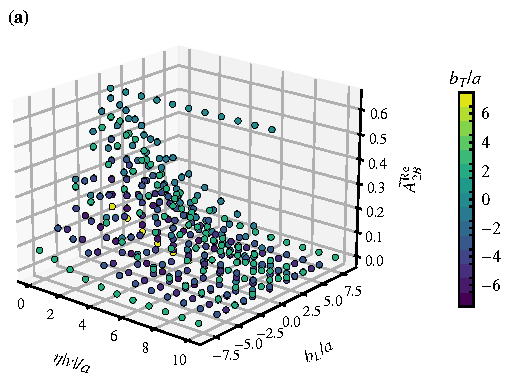
\includegraphics[width=\panelw]{figures/panels/amps/amp3d_ReA2B_PL1.pdf}\hfill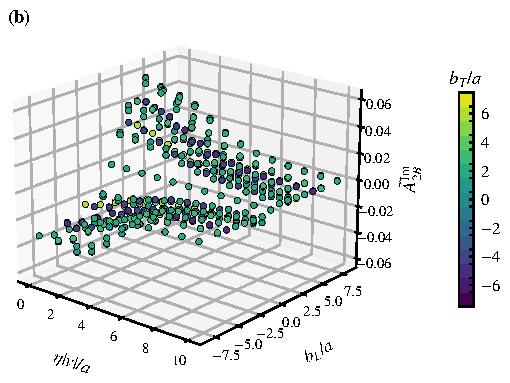
\includegraphics[width=\panelw]{figures/panels/amps/amp3d_ImA2B_PL1.pdf}\\[1ex]
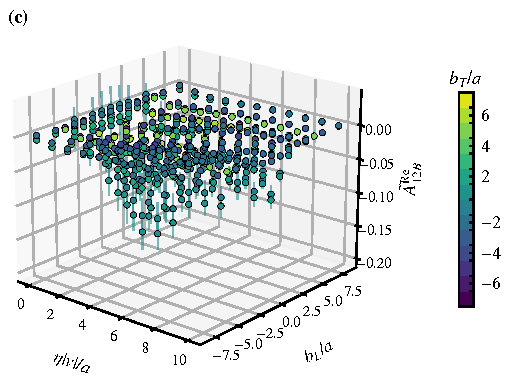
\includegraphics[width=\panelw]{figures/panels/amps/amp3d_ReA12B_PL1.pdf}\hfill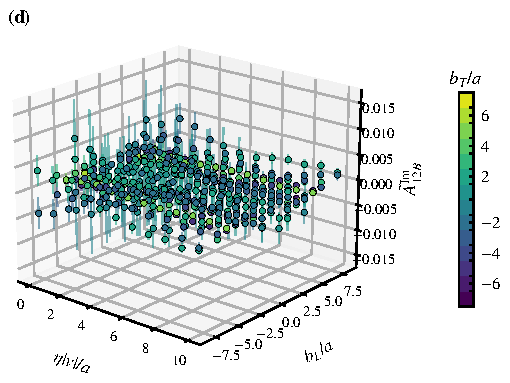
\includegraphics[width=\panelw]{figures/panels/amps/amp3d_ImA12B_PL1.pdf}
\caption{Real (a, c) and imaginary (b, d) parts of $\tAmp_{2B}$ (a, b) and $\tAmp_{12B}$ (c, d) as functions of $\eta|\vect{v}|/a$ and $b_L/a$ for $\vect{P}\cdot a\hat{L}/(2\pi)=\{-1,0,0\}$ ($\hat\zeta=0.090772$). The color labels $b_T/a$.}
\label{fig:BLBT_3D_P1}
\end{figure*}

\begin{figure*}[!t]
\centering
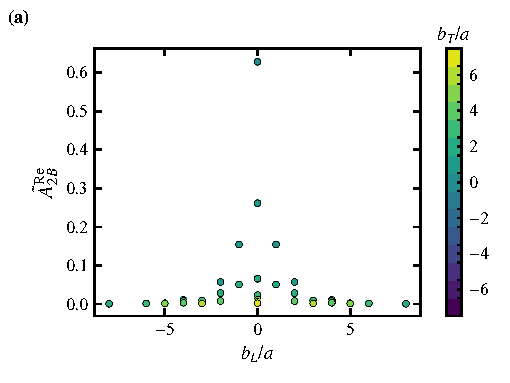
\includegraphics[width=\panelw]{figures/panels/amps/amp2d_eta8_ReA2B_PL1.pdf}\hfill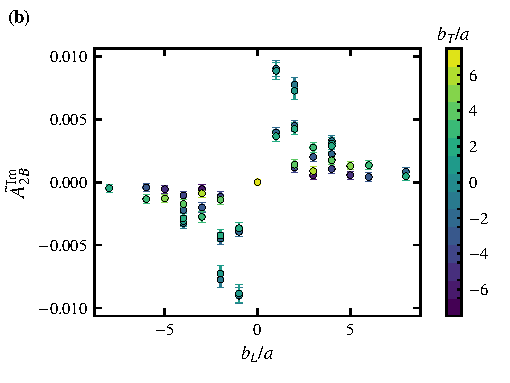
\includegraphics[width=\panelw]{figures/panels/amps/amp2d_eta8_ImA2B_PL1.pdf}\\[1ex]
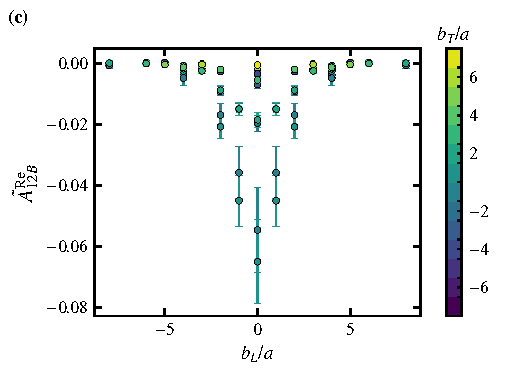
\includegraphics[width=\panelw]{figures/panels/amps/amp2d_eta8_ReA12B_PL1.pdf}\hfill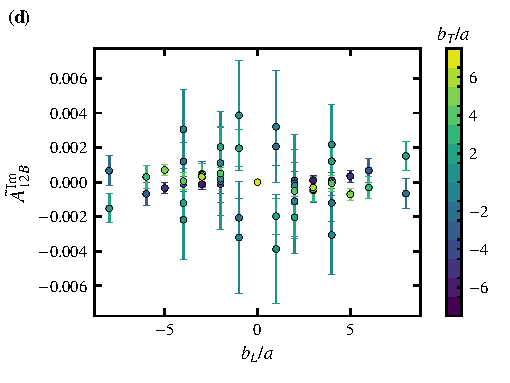
\includegraphics[width=\panelw]{figures/panels/amps/amp2d_eta8_ImA12B_PL1.pdf}
\caption{The amplitudes of Fig.~\ref{fig:BLBT_3D_P1} as functions of $b_L/a$ at fixed $\eta|\vect{v}|/a=8$. The color labels $b_T/a$. Notice the lack of discernible signal in $\tAmp_{12B}^{\text{Im}}$.}
\label{fig:BLBT_eta8_P1}
\end{figure*}

\begin{figure*}[!t]
\centering
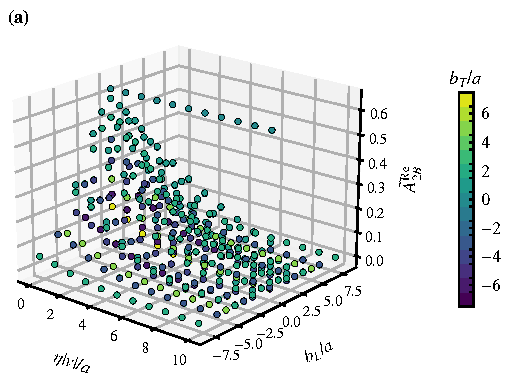
\includegraphics[width=\panelw]{figures/panels/amps/amp3d_ReA2B_PL2.pdf}\hfill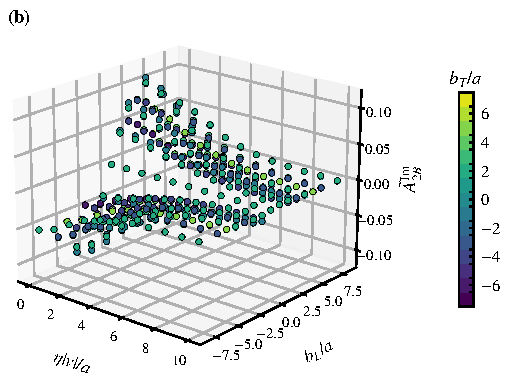
\includegraphics[width=\panelw]{figures/panels/amps/amp3d_ImA2B_PL2.pdf}\\[1ex]
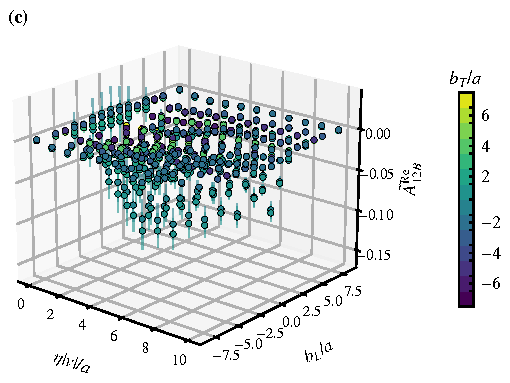
\includegraphics[width=\panelw]{figures/panels/amps/amp3d_ReA12B_PL2.pdf}\hfill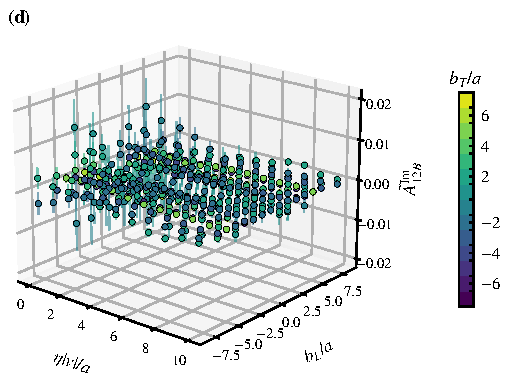
\includegraphics[width=\panelw]{figures/panels/amps/amp3d_ImA12B_PL2.pdf}
\caption{Real (a, c) and imaginary (b, d) parts of $\tAmp_{2B}$ (a, b) and $\tAmp_{12B}$ (c, d) as functions of $\eta|\vect{v}|/a$ and $b_L/a$ for $\vect{P}\cdot a\hat{L}/(2\pi)=\{-2,0,0\}$ ($\hat\zeta=0.294367$). The color labels $b_T/a$.}
\label{fig:BLBT_3D_P2}
\end{figure*}

\begin{figure*}[!t]
\centering
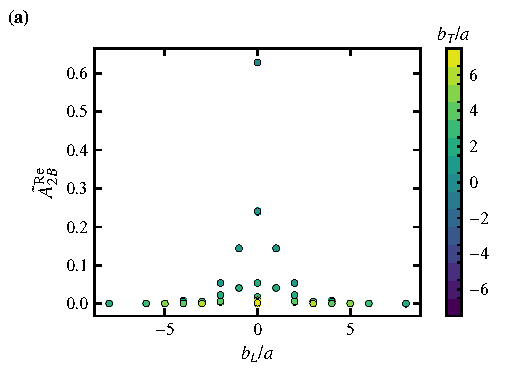
\includegraphics[width=\panelw]{figures/panels/amps/amp2d_eta8_ReA2B_PL2.pdf}\hfill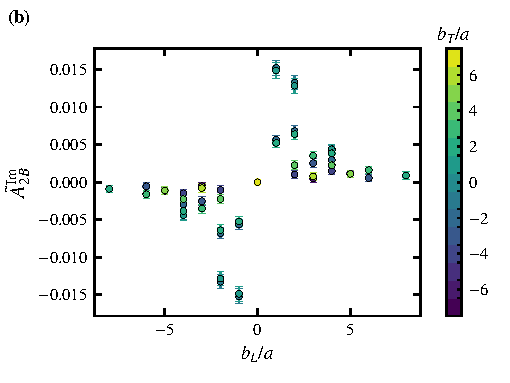
\includegraphics[width=\panelw]{figures/panels/amps/amp2d_eta8_ImA2B_PL2.pdf}\\[1ex]
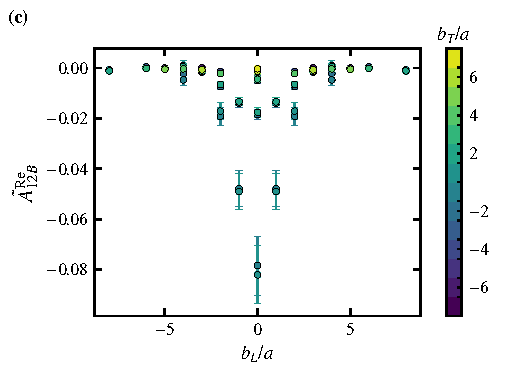
\includegraphics[width=\panelw]{figures/panels/amps/amp2d_eta8_ReA12B_PL2.pdf}\hfill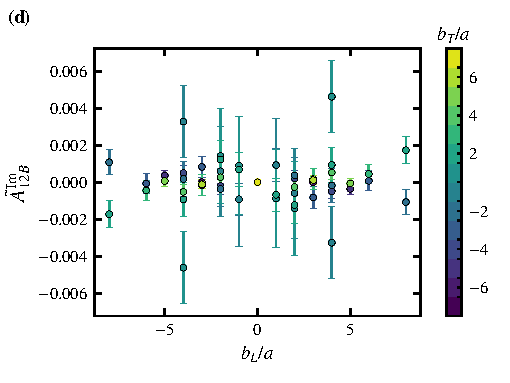
\includegraphics[width=\panelw]{figures/panels/amps/amp2d_eta8_ImA12B_PL2.pdf}
\caption{The amplitudes of Fig.~\ref{fig:BLBT_3D_P2} as functions of $b_L/a$ at fixed $\eta|\vect{v}|/a=8$. The color labels $b_T/a$.}
\label{fig:BLBT_eta8_P2}
\end{figure*}




\section{Results}
\label{sec:results}
\subsection{Fit strategy and data selection}
\label{sec:fit_strategy}

All amplitudes in this section are for the isovector $u-d$ combination. The real unpolarized amplitude $\tAmp_{2B}^{\text{Re}}$ has small statistical errors over the whole lattice parameter space. The imaginary unpolarized amplitude $\tAmp_{2B}^{\text{Im}}$ and the real Sivers amplitude $\tAmp_{12B}^{\text{Re}}$ are noisier, and $\tAmp_{12B}^{\text{Im}}$ was dropped in Sec.~\ref{sec:numerical_amplitudes}. We parametrize the amplitudes in the Cartesian variables $(b_L,b_T,\eta)$, where $b_L=(P\cdot b)/(-P_L)$ and $b_T^2=b^2-b_L^2$. This uses all lattice points and separates the longitudinal from the transverse profile, which the compressed variables $(P\cdot b,b^2)$ do not.

\paragraph{Gaussian profile.}
A 2D Gaussian, $\tAmp^{\text{Re}}_{iB}=\gamma\exp[-\alpha b_L^2-\beta b_T^2]$, becomes $\gamma\exp[-\tfrac{\alpha-\beta}{P_L^2}(P\cdot b)^2-\beta b^2]$ in the invariant variables. The Fourier integral over $P\cdot b$ converges only for $\alpha>\beta$. The fit to $\tAmp^{\text{Re}}_{2B}$ gives $\alpha-\beta=-0.0427(27)$ with $\chi^2/\text{dof}\approx 235$ at $P_L=-1$ (Fig.~\ref{fig:gaussian_fail}), so the Gaussian is both a poor description and not Fourier-integrable.

\paragraph{Short-distance cut.}
At $|\vect{b}|\sim a$ or $2a$ the operator is affected by hypercubic-symmetry breaking, $\mathcal O(a)$ and $\mathcal O(a^2)$ link-path artifacts, and incipient short-distance divergences, while we want the medium-range nonperturbative behavior. We therefore keep only $|\vect{b}|\ge 3a$. Fig.~\ref{fig:short_distance} shows the difference in the data: at fixed $b^2$, the short-distance amplitude rises with $|P\cdot b|$ by about $14\%$ for $b^2/a^2=5$, while it stays flat within errors for $b^2/a^2=20$ and $45$.

\paragraph{Staple extent.}
The Sivers shift requires $\eta\to\infty$. The first-moment study of Ref.~\cite{Musch:2011er} found that the shift reaches a plateau for $|\eta v|=7a\ldots12a$, which indicates that the Sivers and unpolarized TMDs share a common $\eta$ profile that cancels in the ratio. We therefore perform global fits in $(b_L,b_T,\eta)$ over $6\le\eta\le10$.

\begin{figure}
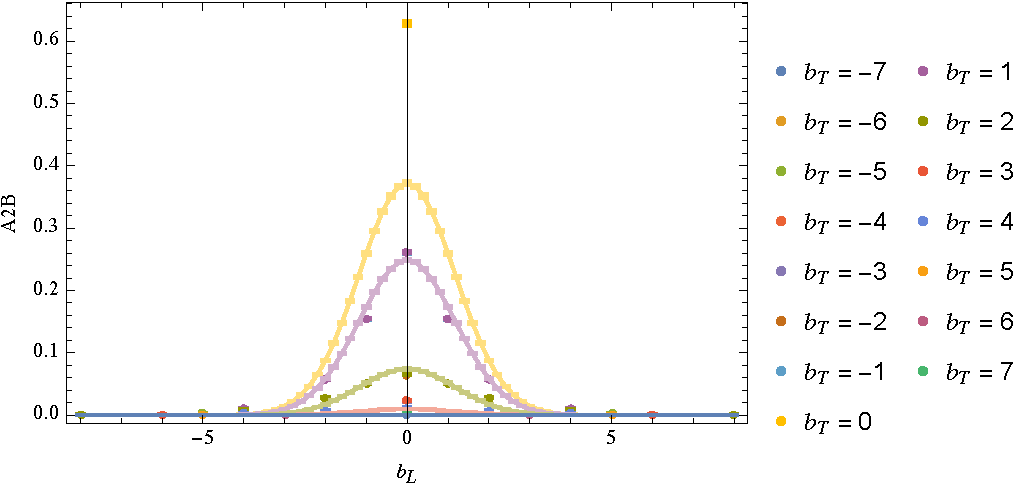
\includegraphics[width=\columnwidth]{figures/results/gaussian_fail_A2B.pdf}
\caption{Failure of the Gaussian model for $\tAmp_{2B}^{\text{Re}}$ at $P_L=-1$ ($\alpha-\beta=-0.0427(27)$, $\chi^2/\text{dof}\approx235$).}
\label{fig:gaussian_fail}
\end{figure}

\begin{figure}
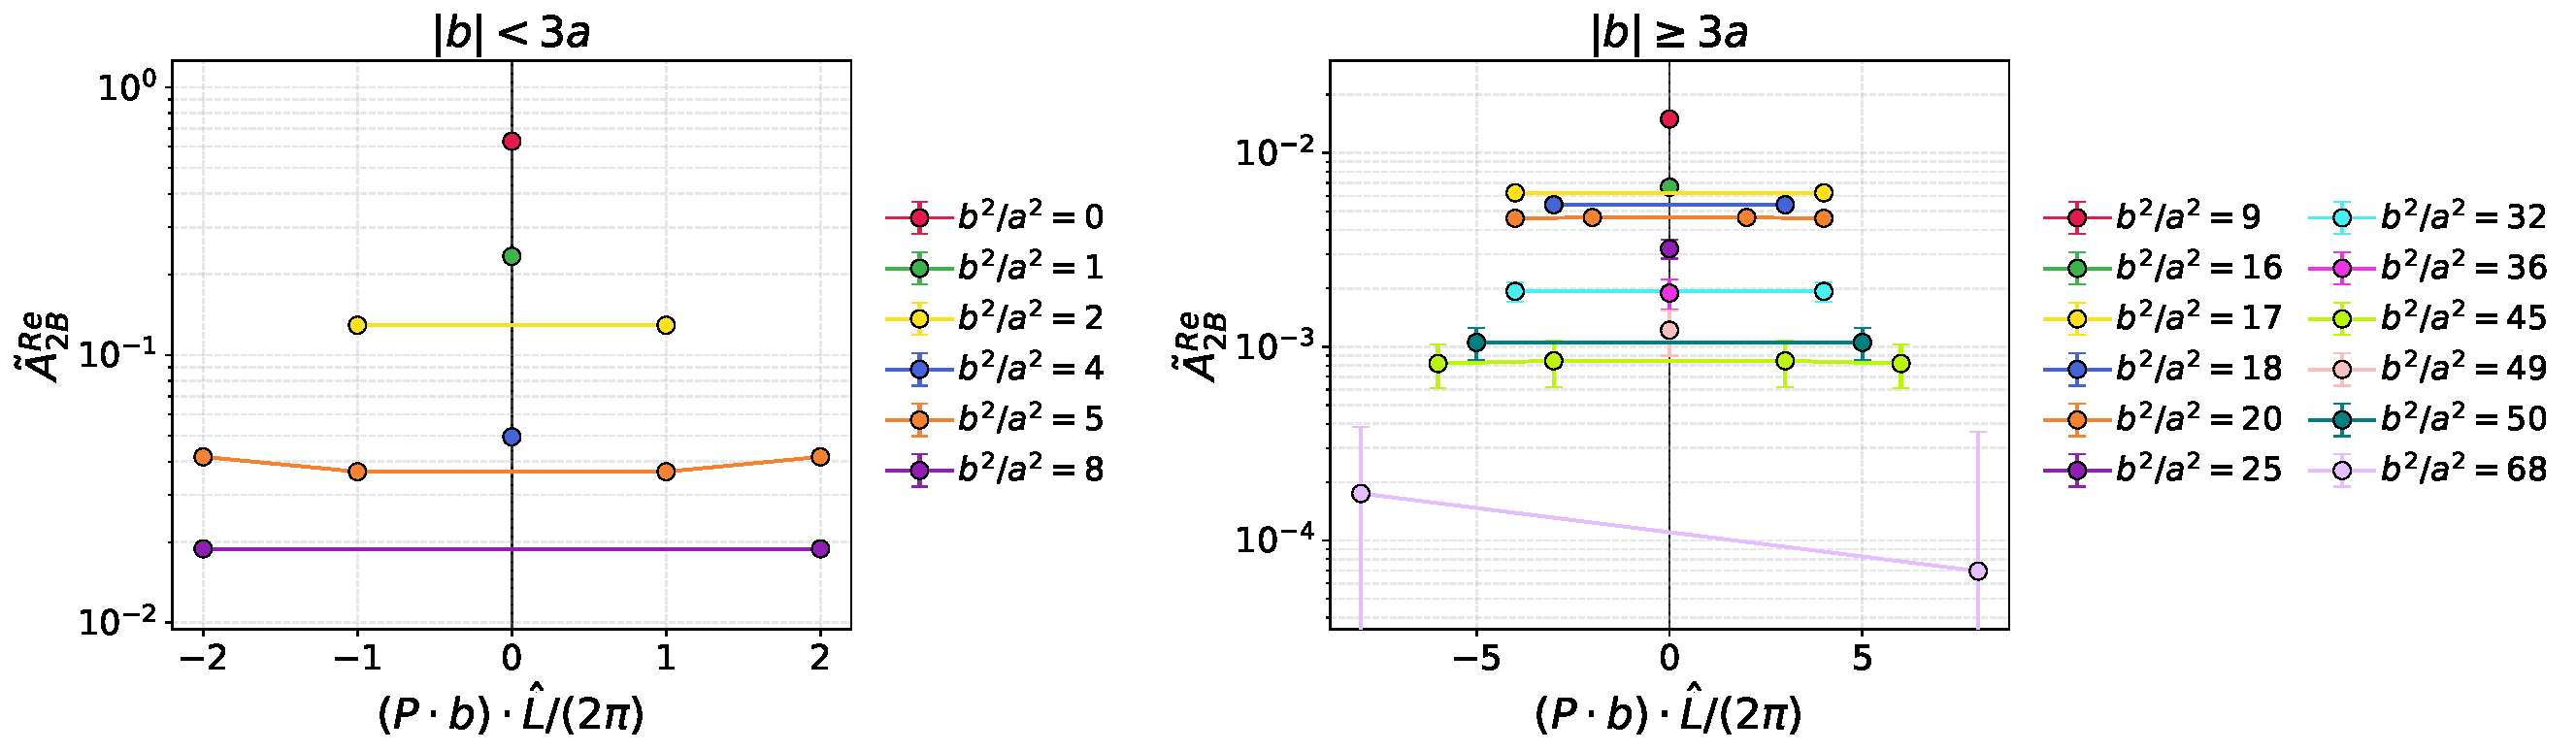
\includegraphics[width=\columnwidth]{figures/results/short_distance.pdf}
\caption{$\tAmp_{2B}^{\text{Re}}$ at $P_L=-1$ and $\eta|\vect v|/a=9$ for $|\vect b|<3a$ (left) and $|\vect b|\ge3a$ (right). Points with equal $b^2$ are connected to guide the eye.}
\label{fig:short_distance}
\end{figure}

\subsection{Global power-law fit}
\label{sec:global_fit}

Symbolic regression with \texttt{PySR}~\cite{Cranmer2023pysr}, using a custom loss that penalizes growth at large $b_L$, points to a power-law tail $(1+b^2)^{-j}$ multiplied by an exponential $e^{-f\eta}$ and never selects a Gaussian profile (Appendix~\ref{app:fit_exploration}). We then explored the $\eta$ dependence of the power-law model, and compared it with exponential and other separable longitudinal-transverse forms (Appendix~\ref{app:fit_exploration}). The separable forms either have a longitudinal coefficient consistent with zero, so that the Fourier transform to $x$ does not exist, or fail for $\tAmp_{2B}^{\text{Im}}$ and $\tAmp_{12B}^{\text{Re}}$. The selected models are
\begin{align}
\tAmp_{2B}^{\text{Re}}&=\frac{a\,e^{-f\eta}}{\big[1+\big(d+c\,(1-\tfrac{k_1}{\eta}-\tfrac{k_2}{\eta^2})\big)b_L^2+d\,b_T^2\big]^{j}}\,,\label{eq:model_ReA2B}\\
\tAmp_{2B}^{\text{Im}}&=\frac{a''\,b_L\,e^{-f\eta}}{\big[1+(c''+d'')b_L^2+d''b_T^2\big]^{j''}}\,,\label{eq:model_ImA2B}\\
\tAmp_{12B}^{\text{Re}}&=\frac{-a'\,e^{-f\eta}}{\big[1+(c'+d')b_L^2+d'b_T^2\big]^{j'}}\,.\label{eq:model_ReA12B}
\end{align}
The $\eta$ dependence of $c$ in $\tAmp_{2B}^{\text{Re}}$ was chosen among several candidates with equal $\chi^2/\text{dof}$ by requiring that the antiquark region $x\lesssim-0.2$ of $\tilde f_1^{(0)}$ is suppressed at large momentum and that the $x$-integrated results agree with earlier first-moment calculations~\cite{Musch:2011er,Yoon:2017qzo}. For $\tAmp_{12B}^{\text{Re}}$, the slopes of $c$ and $d$ against $\eta$ are consistent with zero within about $1\sigma$, and for $d$ of $\tAmp_{2B}^{\text{Re}}$ the slope is $0.00122(87)$. For $\tAmp_{2B}^{\text{Im}}$ the slope of $d$ is within $1.5\sigma$ of zero and that of $c$ is about $2\sigma$ from zero. We keep these parameters constant in $\eta$ to avoid overfitting.

Since $e^{-f\eta}$ does not depend on $P\cdot b$, it cancels between numerator and denominator of the Sivers shift, Eq.~\eqref{eq:sivers_shift_xdep}, when it is shared by the three amplitudes. We therefore fit the three amplitudes simultaneously at each momentum with one common $f$, minimizing the correlated $\chi^2$ with the full Jackknife covariance matrix~\cite{Boram2011Covariance}, which includes correlations between different $(b_L,b_T,\eta)$ points and between the three amplitudes. The fits use \texttt{lsqfit}~\cite{Lepage:2001ym}. The global $\chi^2/\text{dof}$ is $1.85(10)$, $1.197(85)$, $0.712(66)$ and $0.434(51)$ for $P_L=-1,\ldots,-4$, and the fitted parameters are listed in Table~\ref{tab:fit_params} of Appendix~\ref{app:fit_exploration}. Fig.~\ref{fig:fit_example} compares the fit with the data for $P_L=-4$ at $\eta|\vect v|/a=8$.

\begin{figure*}
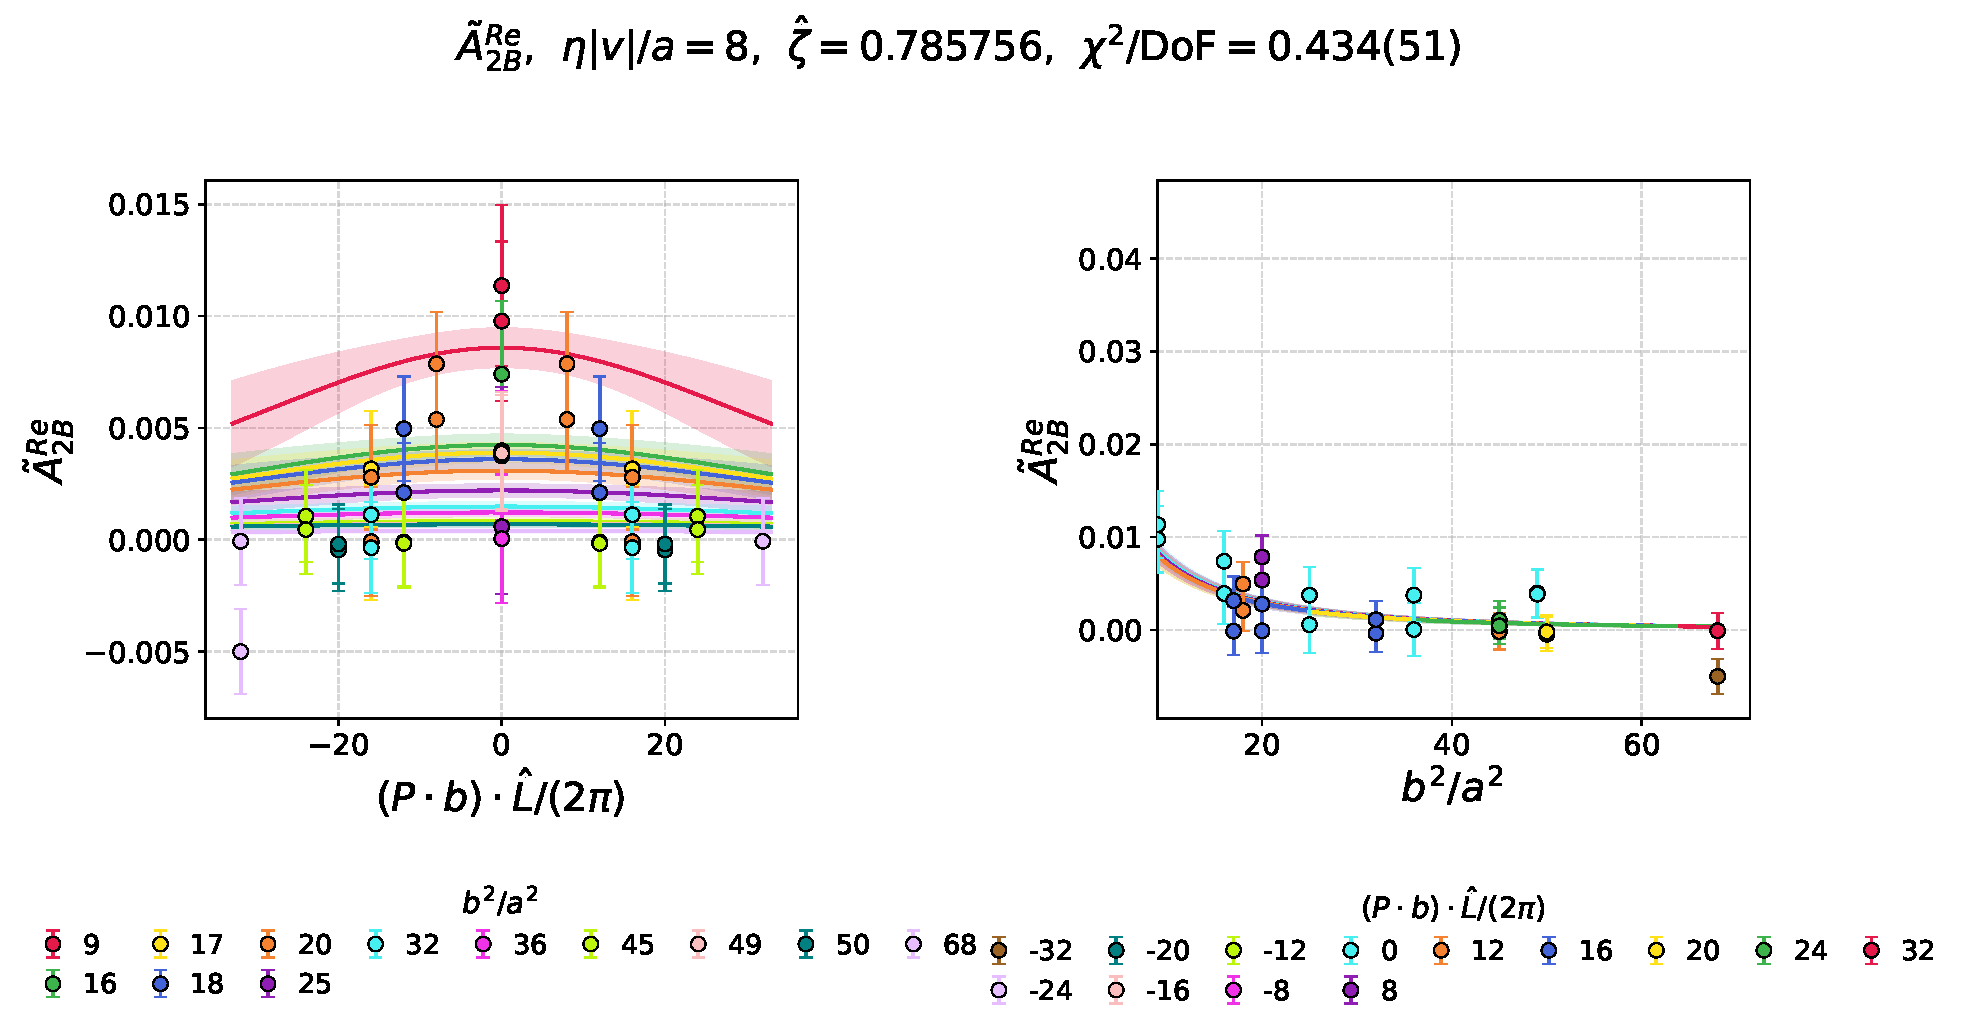
\includegraphics[width=0.32\textwidth]{figures/results/fit_ReA2B_PL-4_eta8.pdf}\hfill
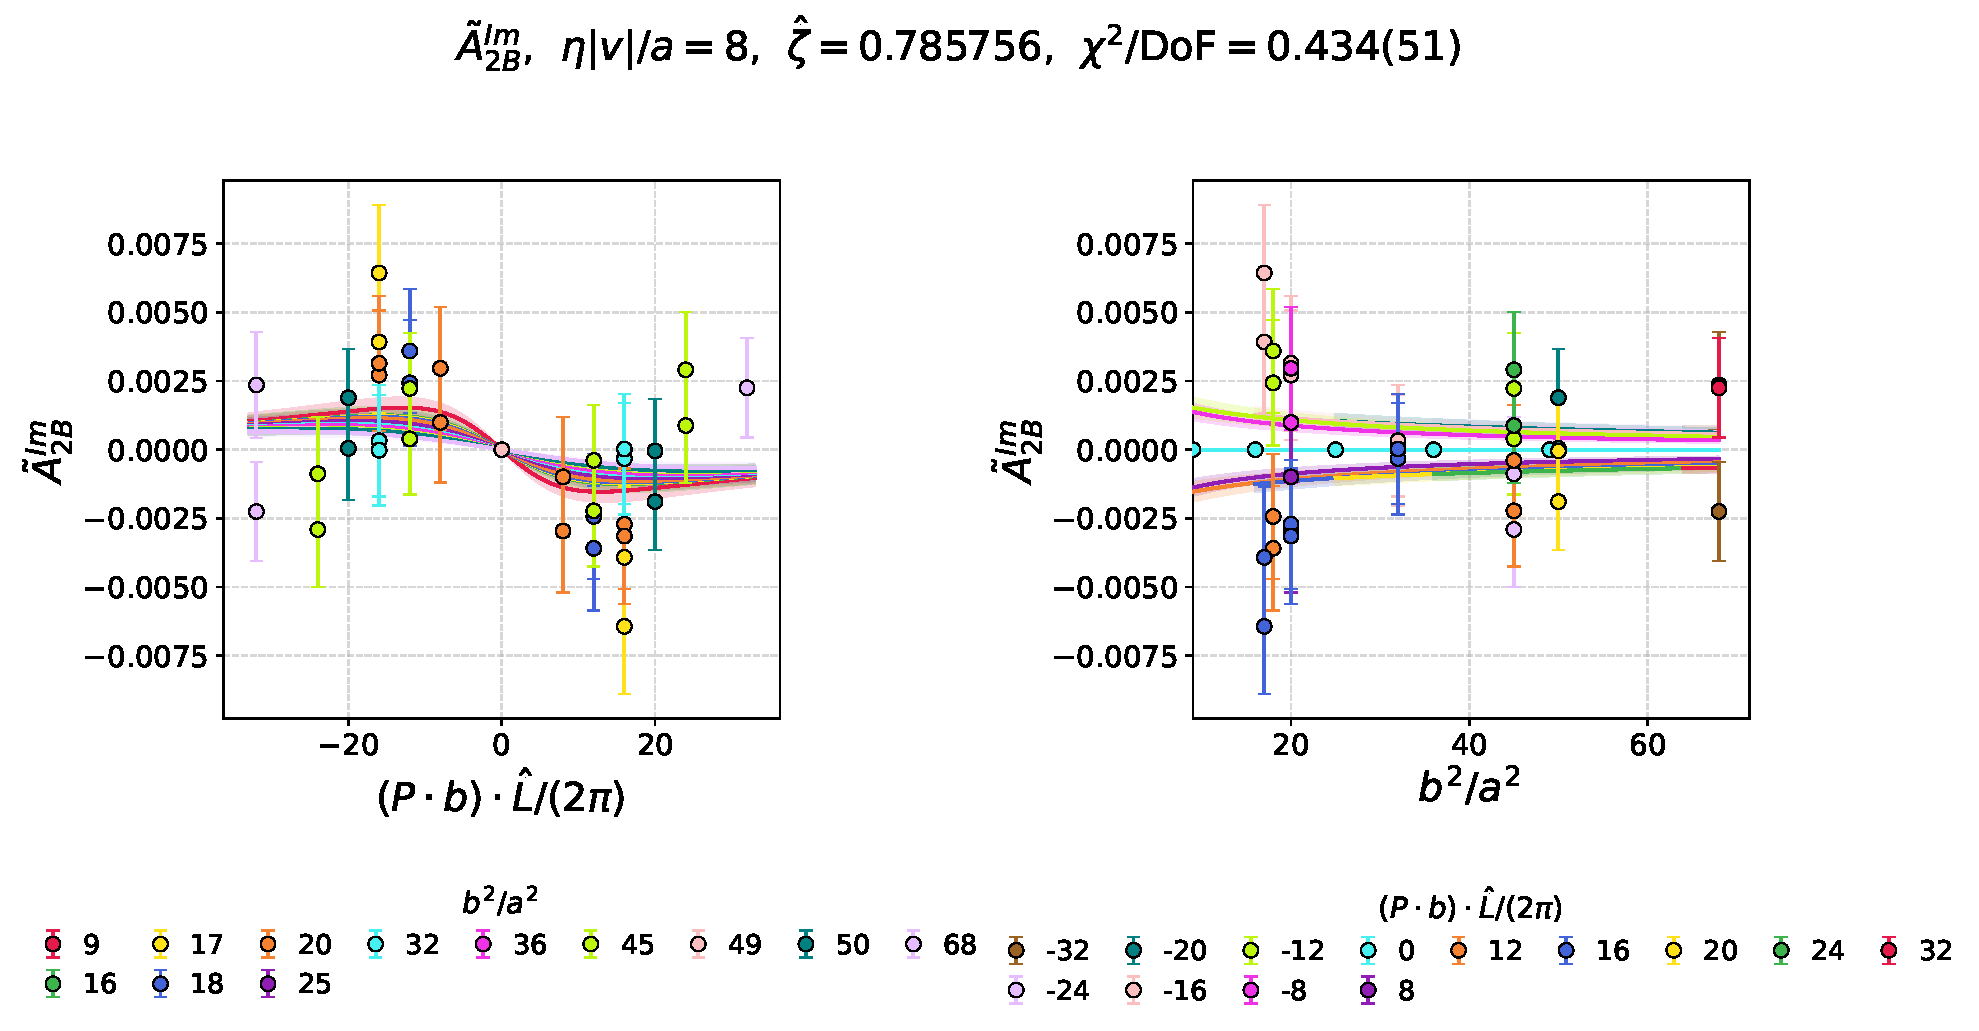
\includegraphics[width=0.32\textwidth]{figures/results/fit_ImA2B_PL-4_eta8.pdf}\hfill
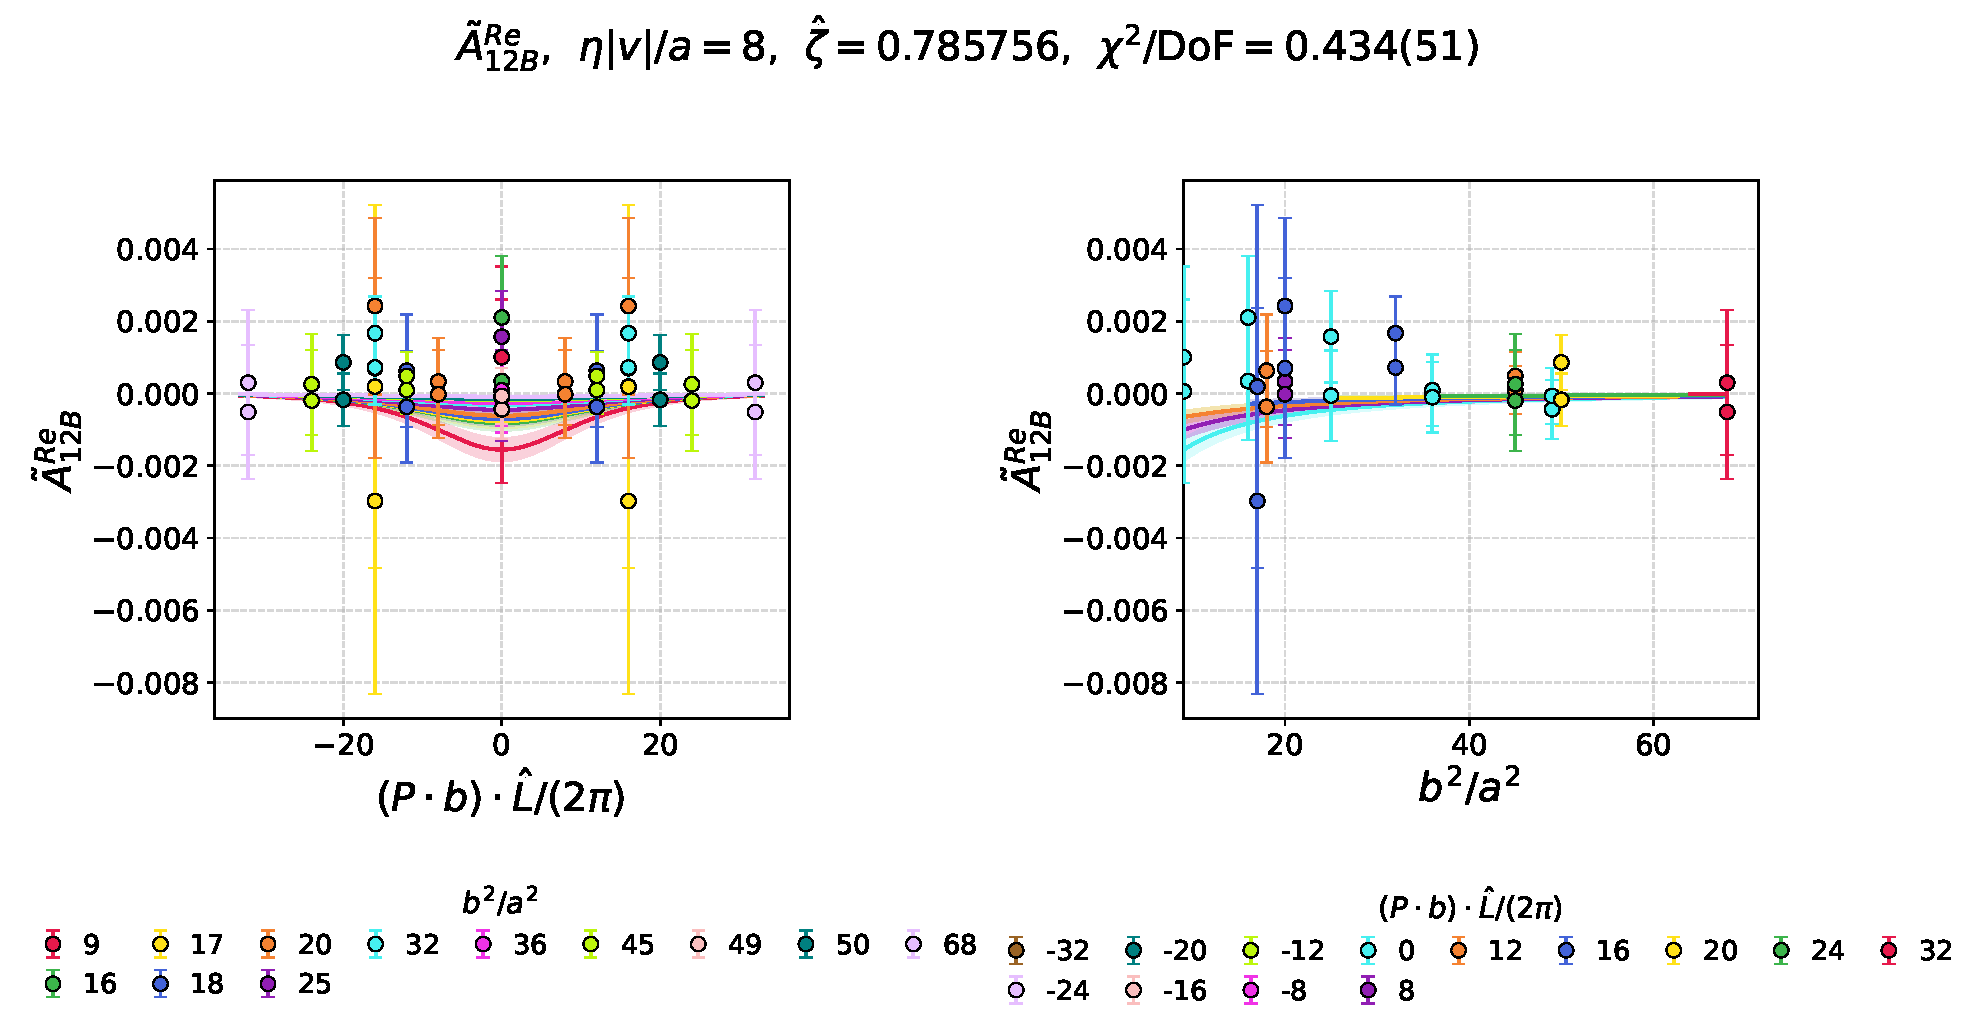
\includegraphics[width=0.32\textwidth]{figures/results/fit_ReA12B_PL-4_eta8.pdf}
\caption{Simultaneous fit for $P_L=-4$ at $\eta|\vect v|/a=8$ in the variables $(P\cdot b,b^2)$: $\tAmp_{2B}^{\text{Re}}$, $\tAmp_{2B}^{\text{Im}}$ and $\tAmp_{12B}^{\text{Re}}$ (left to right).}
\label{fig:fit_example}
\end{figure*}

\subsection{Extrapolation to $\hat\zeta\to\infty$}
\label{sec:zeta_extrapolation}

The simulated momenta $P_L=-1,\ldots,-4$ correspond to $\hat\zeta=0.090772$, $0.294367$, $0.539684$, $0.785756$, far from the $\hat\zeta\gg1$ regime relevant for comparison with factorization-based phenomenology. At fixed $|\vect b_T|=3a\approx0.34$~fm, the reconstructed amplitudes, the TMD combinations $\tilde f_1^{(0)}=2\tAmp_{2B}^{[x]}$ and $\tilde f_{1T}^{\perp(1)}=-2\tAmp_{12B}^{[x]\text{Re}}$, and the Sivers shift all vary systematically with $1/\hat\zeta$. Perturbative TMD evolution~\cite{Aybat:2011zv} suggests that ratios of TMDs become independent of $\hat\zeta$ as $\hat\zeta\to\infty$, which is the physical limit for the Sivers shift, where the soft factor cancels.

We extrapolate the fit parameters themselves rather than the amplitudes point by point in $x$. We exclude $P_L=-1$ ($1/\hat\zeta=11.02$), which lies far from the other three ($1/\hat\zeta=3.40$, $1.85$, $1.27$) and would dominate the extrapolated intercept. The parameters $c$ of the three amplitudes are first rescaled by $1/P_L^2$, and the parameter of the odd amplitude $\tAmp_{2B}^{\text{Im}}$ multiplying $b_L$ by $1/P_L$, so that they multiply powers of the invariant $P\cdot b$ at all momenta. We tested
\begin{equation}
p(\hat\zeta)=c_p+\frac{d_p}{\hat\zeta}\quad\text{and}\quad p(\hat\zeta)=c_p+\frac{d_p}{\hat\zeta^{2}}
\label{eq:zeta_ansatz}
\end{equation}
as in Ref.~\cite{Musch:2011er} with correlated Jackknife fits to the three momenta. The quadratic form gives a lower $\chi^2/\text{dof}$ for the parameters and we adopt it throughout (Fig.~\ref{fig:param_extrap}). The extrapolated value of each parameter is the intercept $c_p$. With only three momenta and two parameters per fit, this extrapolation has one degree of freedom and its systematic uncertainty is not captured by the Jackknife errors.

Reconstructing the amplitudes from the extrapolated parameters gives $\tilde f_1^{(0)}$, $\tilde f_{1T}^{\perp(1)}$ and the Sivers shift at $\hat\zeta\to\infty$ (Fig.~\ref{fig:extrap_sivers}). At $|\vect b_T|=0.34$~fm, $\langle k_y\rangle_{TU}$ peaks at about $0.21$~GeV at small $x$ and falls to near zero by $x\approx0.5$, while $x\langle k_y\rangle_{TU}$ peaks at about $0.02$~GeV near $x\approx0.15$. The overall sign reverses between the SIDIS and DY limits and the magnitude is unchanged. The extrapolated curve differs from all three finite-momentum curves that enter it, including the one at $P_L=-4$, so the extrapolation captures momentum dependence beyond the largest simulated momentum. Fig.~\ref{fig:extrap_sivers_3D} shows the dependence on $|\vect b_T|$ between $3a\approx0.34$~fm and $\sqrt{68}\,a\approx0.94$~fm.

Table~\ref{tab:integrals} lists the $x$-integrals of the extrapolated amplitudes at $|\vect b_T|=3a$. Integrating over $[-\infty,\infty]$ and $[-1,1]$ gives the same results within errors, so the truncation at $|x|=1$ is negligible. The imaginary term $\int dx\,\tAmp^{[x]\text{Im}}_{2B}$ vanishes over the symmetric ranges and has opposite sign for the quark and antiquark ranges, as required by its odd parity. The first four rows are unrenormalized and the multiplicative renormalization cancels only in the ratio in the last row.

\begin{table*}
\caption{$x$-integrals of the extrapolated ($\hat\zeta\to\infty$) amplitudes at $|\vect b_T|=3a\approx0.34$~fm for four integration ranges. The first four rows are unrenormalized.}
\label{tab:integrals}
\begin{ruledtabular}
\begin{tabular}{lcccc}
Integral & $[-\infty,\infty]$ & $[-1,1]$ & $[-1,0]$ & $[0,1]$ \\
\hline
$\int\!dx\,\tAmp^{[x]\text{Re}}_{2B}$ & $0.751(79)$ & $0.751(80)$ & $0.375(40)$ & $0.375(40)$ \\
$\int\!dx\,\tAmp^{[x]\text{Im}}_{2B}$ & $6(96)\!\times\!10^{-17}$ & $3(24)\!\times\!10^{-16}$ & $0.165(27)$ & $-0.169(29)$ \\
$\int\!dx\,\tilde f_1^{(0)}$ & $1.50(16)$ & $1.50(16)$ & $0.421(81)$ & $1.09(11)$ \\
$\int\!dx\,\tilde f_{1T}^{\perp(1)}$ & $0.302(53)$ & $0.302(53)$ & $0.151(27)$ & $0.151(27)$ \\
$\langle k_y\rangle_{TU}$ (GeV) & $0.217(38)$ & $0.217(38)$ & $0.387(89)$ & $0.150(26)$ \\
\end{tabular}
\end{ruledtabular}
\end{table*}

\begin{figure*}
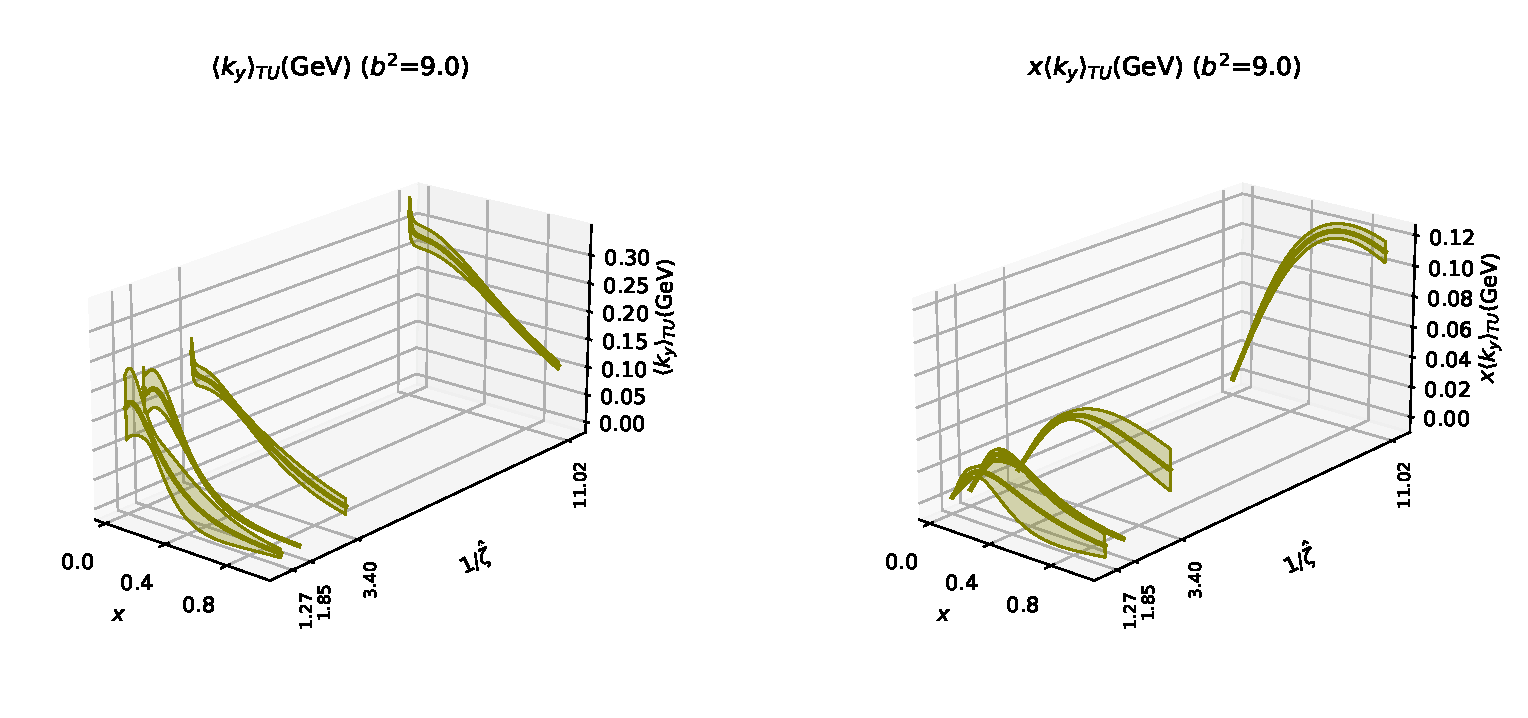
\includegraphics[width=0.9\textwidth]{figures/results/zetahat_slices_sivers.pdf}
\caption{Sivers shift $\langle k_y\rangle_{TU}$ and $x\langle k_y\rangle_{TU}$ at $|\vect b_T|=3a\approx0.34$~fm for the four simulated momenta, against $x$ and $1/\hat\zeta$ ($x\ge0$).}
\label{fig:zetahat_slices}
\end{figure*}

\begin{figure*}
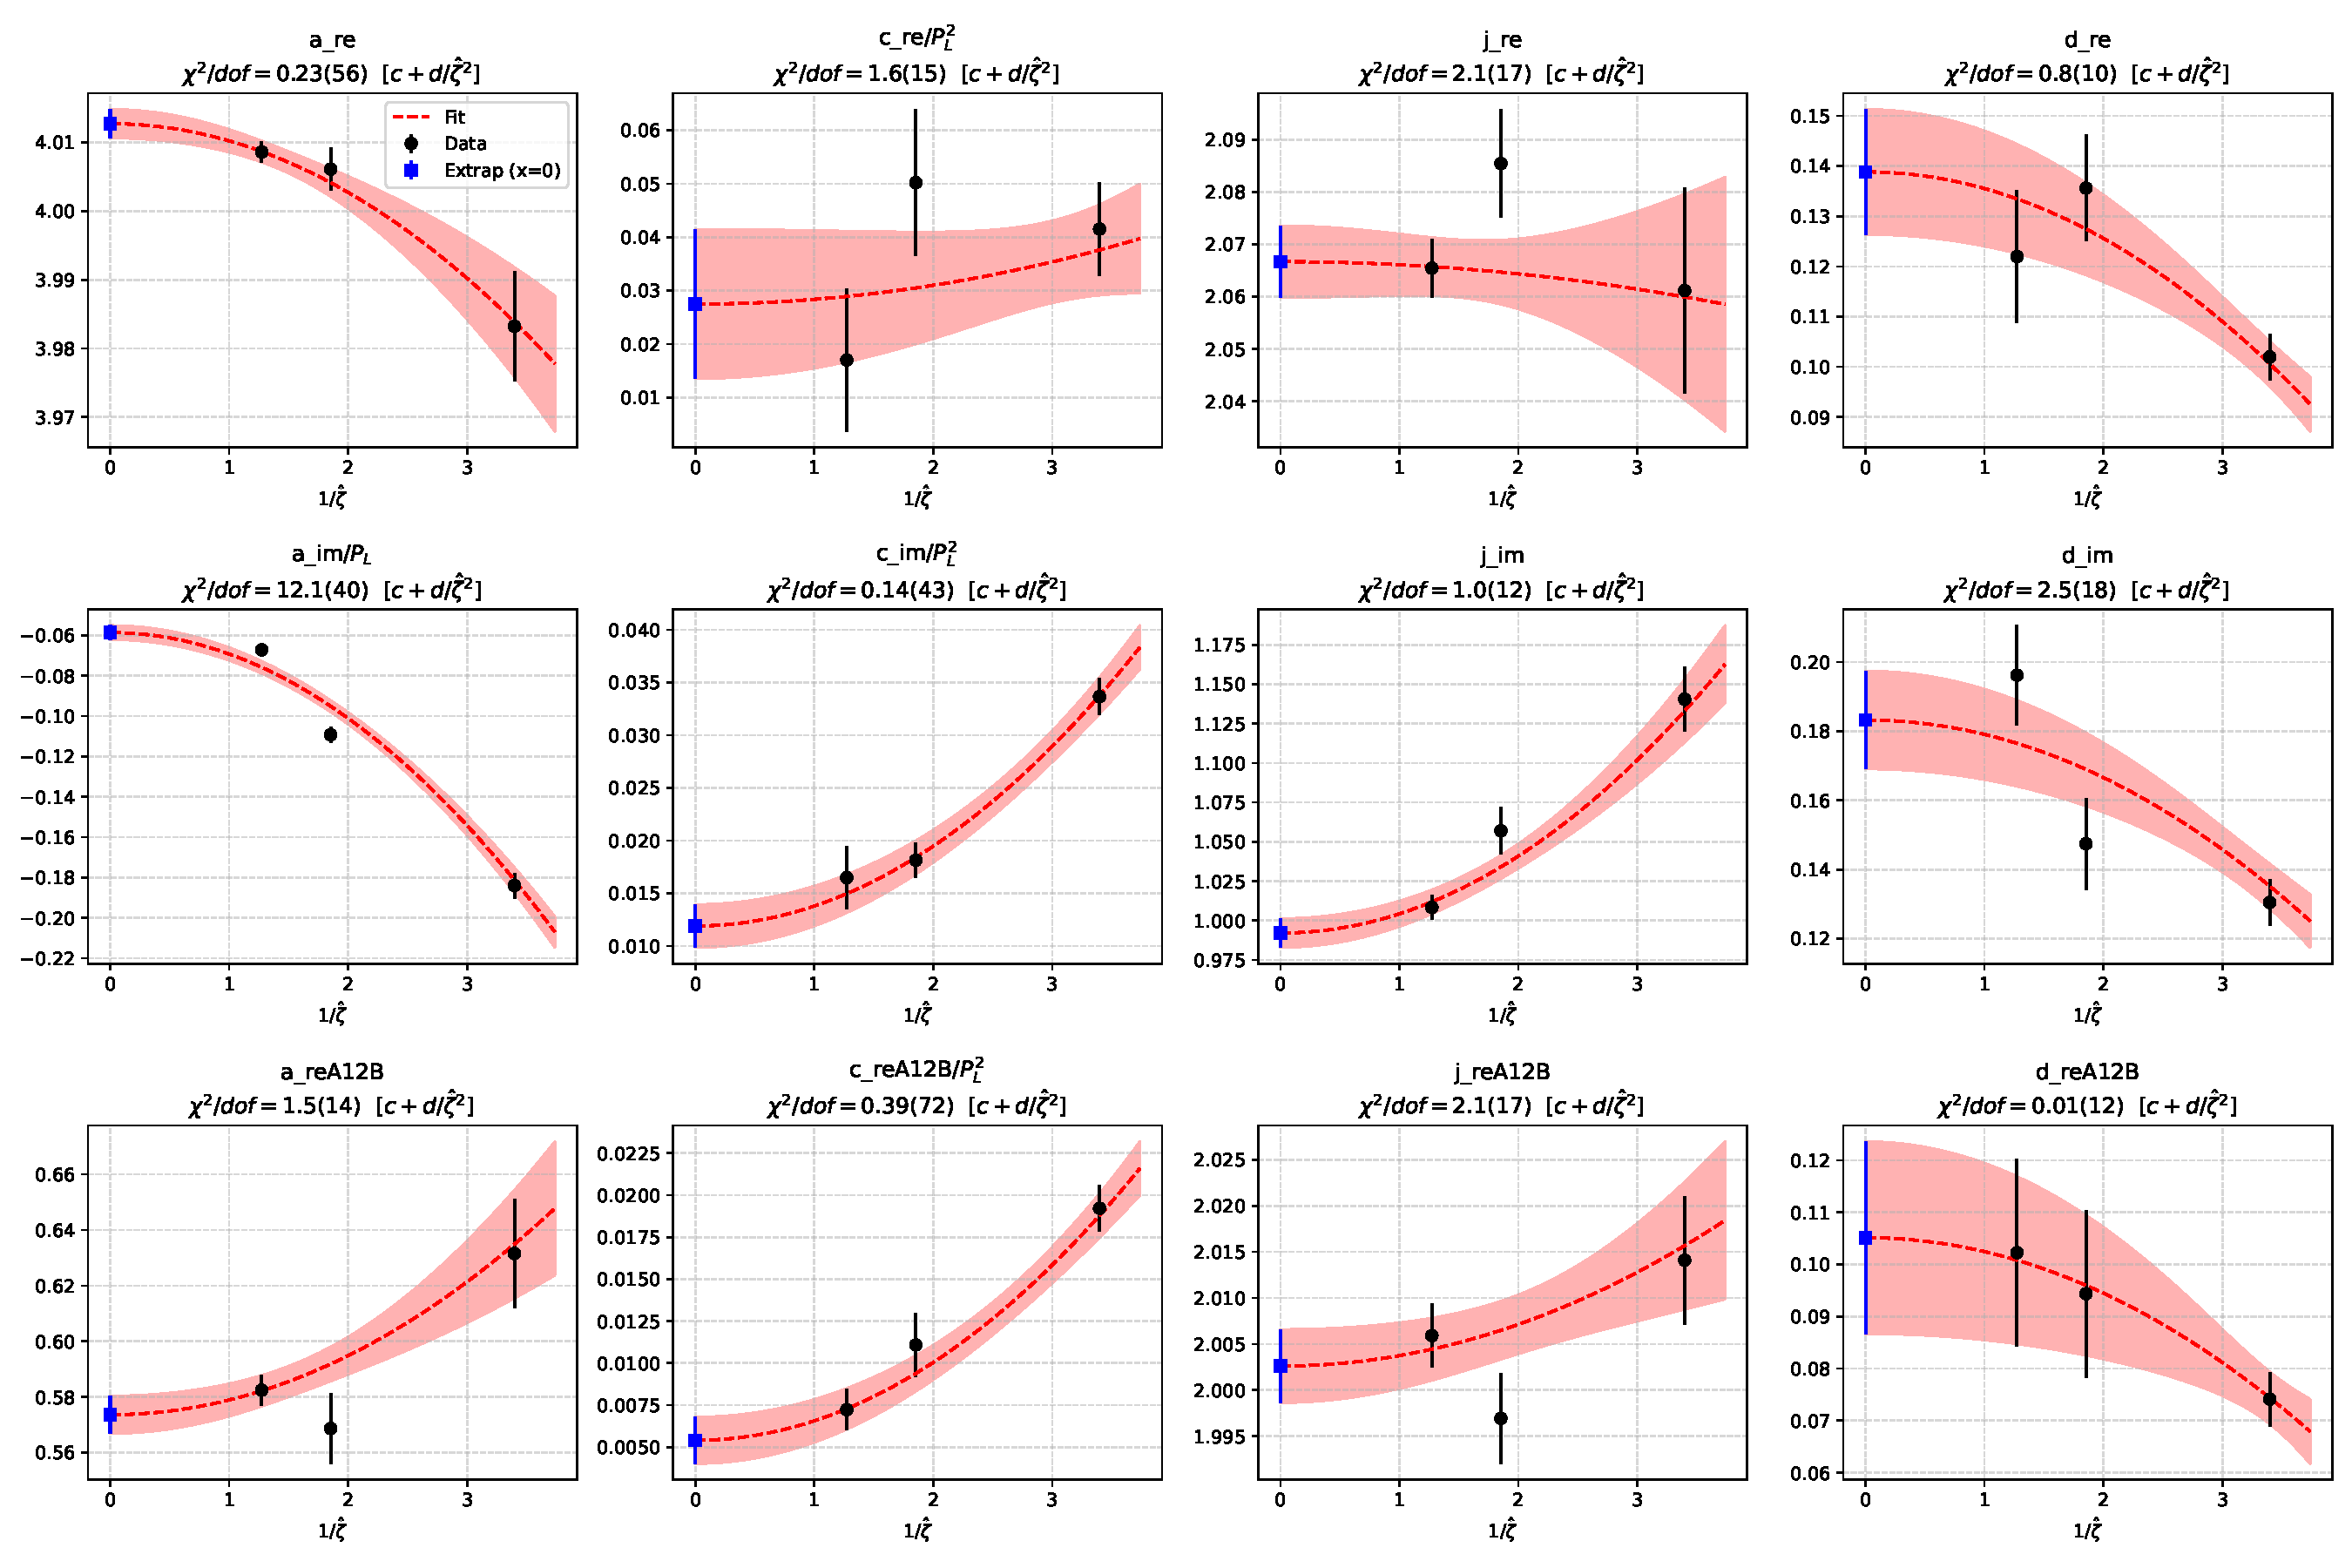
\includegraphics[width=0.75\textwidth]{figures/results/param_extrapolation.pdf}
\caption{Extrapolation of the twelve fit parameters to $\hat\zeta\to\infty$ using $P_L=-2,-3,-4$ (black), with the ansatz $c_p+d_p/\hat\zeta^2$ (red dashed, band) and the extrapolated value (blue square). Each panel title gives the Jackknife $\chi^2/\text{dof}$. The parameters $c$ are shown rescaled by $1/P_L^2$ and the coefficient of $b_L$ in $\tAmp_{2B}^{\text{Im}}$ by $1/P_L$.}
\label{fig:param_extrap}
\end{figure*}

\begin{figure*}
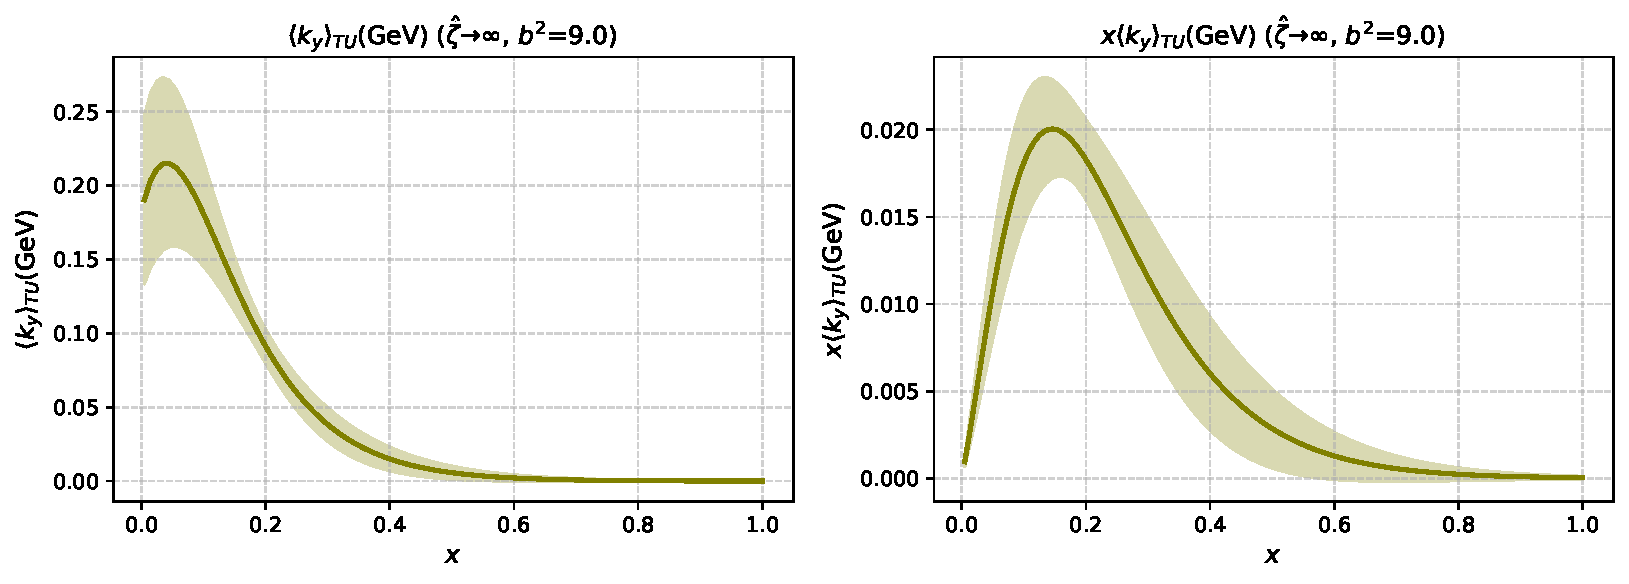
\includegraphics[width=0.9\textwidth]{figures/results/extrap_sivers.pdf}
\caption{Isovector Sivers shift $\langle k_y\rangle_{TU}$ and $x\langle k_y\rangle_{TU}$ at $\hat\zeta\to\infty$ for $|\vect b_T|=3a\approx0.34$~fm. Bands are Jackknife uncertainties propagated from the extrapolated parameters.}
\label{fig:extrap_sivers}
\end{figure*}

\begin{figure}
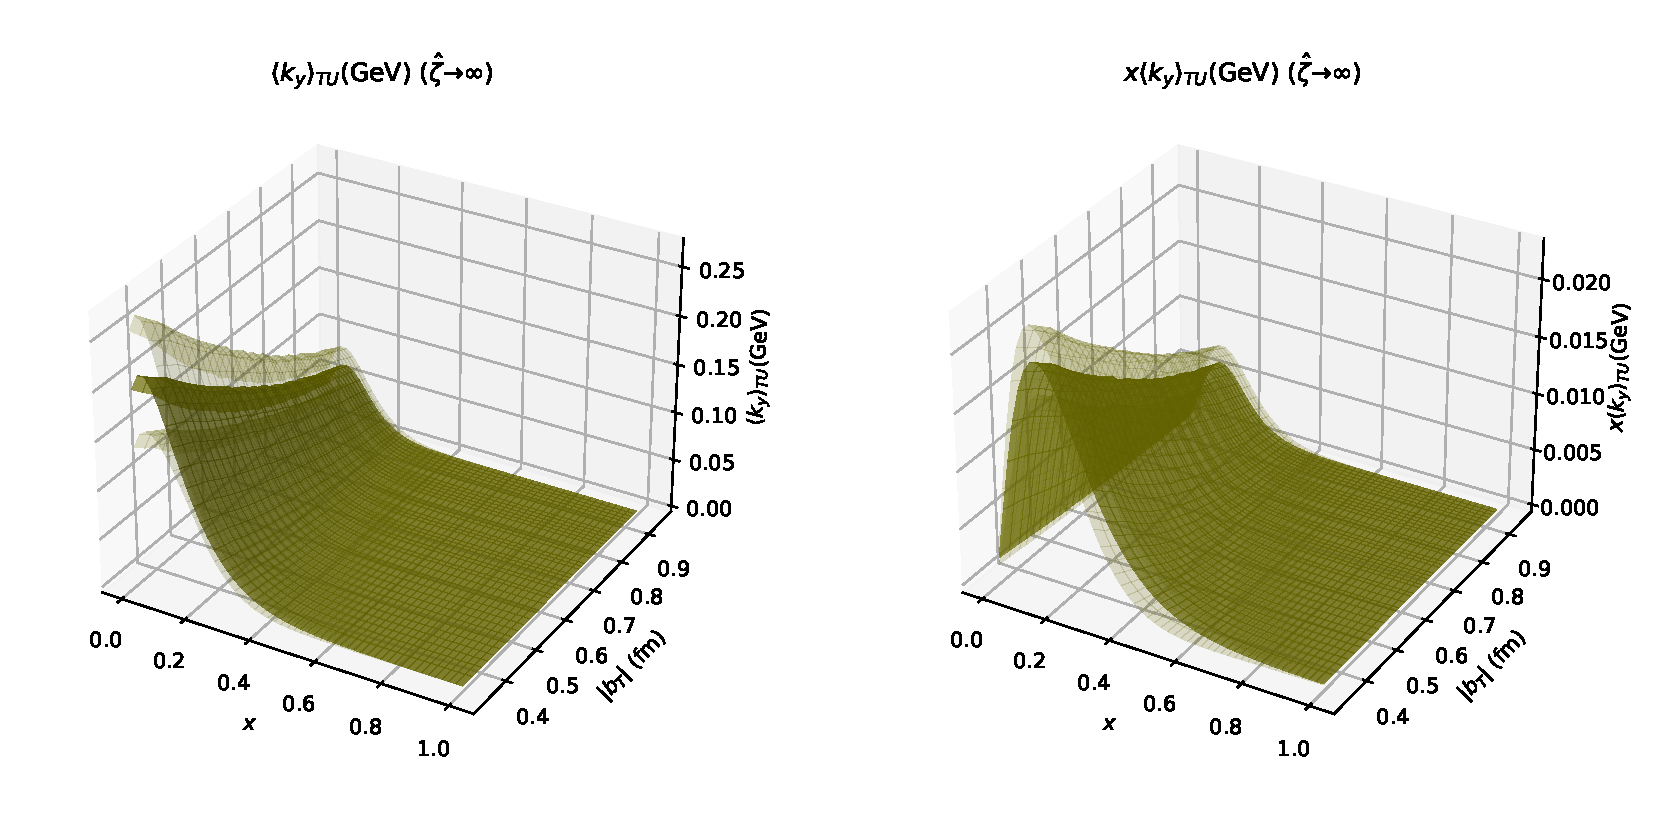
\includegraphics[width=\columnwidth]{figures/results/extrap_sivers_3D.pdf}
\caption{Extrapolated Sivers shift as a function of $x\ge0$ and $|\vect b_T|$ from $0.34$ to $0.94$~fm.}
\label{fig:extrap_sivers_3D}
\end{figure}

\subsection{Factorization in $x$ and $|\vect b_T|$}
\label{sec:factorization}

The global fit couples $(P\cdot b)$ and $b^2$, and the selected models are not products of separate functions of the two variables. The question is how far a factorized description, common in phenomenology, can nonetheless approximate the result. A recent symbolic-regression extraction of the unpolarized TMD from Drell-Yan data finds a mild but genuine $x$-$b_T$ correlation rather than strict separability~\cite{Granger:2026symb}.

\paragraph{Lattice data.}
We first test the data at finite momentum for the form $\tAmp(P\cdot b,b^2)=F(P\cdot b)G(b^2)$. Under factorization, $T=\tAmp(P\cdot b,b^2)/\tAmp(P\cdot b=4,b^2)$ is flat in $b^2$ and $B=\tAmp(P\cdot b,b^2)/\tAmp(P\cdot b,b^2=18)$ is flat in $P\cdot b$. After the cut $b^2\ge9$, at $\eta|v|/a=8$ and $P_L=-1$ only three values of $P\cdot b$ ($0$, $3$ and $4$) have more than one $b^2$, and no two of these rows share two $b^2$ values. We therefore interpolate in $b^2$ onto a common grid $b^2=18,20,25,32$ (quadratic or linear, with no extrapolation) and find that $T$ is flat near $P\cdot b=0$ but increases monotonically for $P\cdot b=3$, and that $B$ is not flat (Fig.~\ref{fig:fact_data}). Because of the sparse sampling and the interpolation this is only a qualitative test, which suggests that factorization is not perfect.

\paragraph{Extrapolated Sivers shift.}
For the extrapolated shift $\langle k_y\rangle_{TU}(x,|\vect b_T|)$ we find the pair $g(x)h(|\vect b_T|)$ that minimizes $J=\int dx\,d|\vect b_T|\,(f-gh)^2$ by iterating the self-consistent equation that follows from the stationarity conditions in $g$ and $h$ (Appendix~\ref{app:factorization_metric}), and report the relative distance $\sqrt{J/N}$, with $N=\int dx\,d|\vect b_T|\,f^2$. This is zero for exact factorization. We apply the iteration to each Jackknife sample on a discrete grid of $60$ points in $|\vect b_T|\in[0.3421,0.9403]$~fm and for four $x$-windows. Table~\ref{tab:fact_sivers} shows relative distances of $5.7$--$7.6\%$, nonzero well outside the Jackknife errors and stable as the window moves away from $x=0$. The Sivers shift is therefore close to, but not exactly, factorized.

Factorization in the fit ansatz would require the order $j_X$ and width $d_X$ of the Bessel-type Fourier transform to coincide for the three amplitudes. The extrapolated values are $j_{\text{re}}=2.0667(69)$, $j_{\text{im}}=0.9921(92)$, $j_{\text{reA12B}}=2.0026(40)$ and $d_{\text{re}}=0.139(12)$, $d_{\text{im}}=0.183(14)$, $d_{\text{reA12B}}=0.105(18)$. The $j$ of the imaginary amplitude differs clearly from the other two, and the $d_X$ are resolved from each other well outside their errors, which accounts for the residual.

Ratios at fixed $|\vect b_T|$ or fixed $x$ show the same effect directly (Figs.~\ref{fig:fact_ratio_x} and~\ref{fig:fact_ratio_bT}): under exact factorization $R_b(x)=\langle k_y\rangle_{TU}(x,|\vect b_T|)/\langle k_y\rangle_{TU}(x,|\vect b_T|_{\rm ref})$ is flat in $x$ and $R_x(|\vect b_T|)=\langle k_y\rangle_{TU}(x,|\vect b_T|)/\langle k_y\rangle_{TU}(x_{\rm ref},|\vect b_T|)$ is flat in $|\vect b_T|$, and neither is. The same non-flat pattern is present at each finite momentum, so it is a feature of the fitted amplitudes and not of the $\hat\zeta\to\infty$ extrapolation.

\paragraph{Amplitude level.}
The same distance test applied to the individual extrapolated amplitudes for $x\in[0,1]$ gives relative distances of $8$--$19\%$, larger than the $5.7\%$ for the Sivers shift in the same window, so the ratio partially cancels the non-factorized behavior. All residuals shrink as the $x$-window narrows away from $x=0$ (Appendix~\ref{app:factorization_metric}).

We conclude that a factorized form $F(x)G(|\vect b_T|)$ is a good, but not exact, approximation to the extracted Sivers shift, to about $5.7$--$7.6\%$ in the relative $L_2$ sense. This agrees qualitatively with Ref.~\cite{Granger:2026symb}, where an $x$-$b_T$ cross term survives a sparsity prior. The two results are complementary rather than directly comparable: that extraction constrains the TMD for $b_T\lesssim2.5$~GeV$^{-1}$ ($\approx0.49$~fm), our range $0.34$--$0.94$~fm extends well beyond it, and our individual amplitudes are unrenormalized so that only the Sivers-shift ratio is a physical quantity.

\begin{table}
\caption{Relative distance of the extrapolated Sivers shift from its best factorized form $F(x)G(|\vect b_T|)$ for $|\vect b_T|\in[0.3421,0.9403]$~fm.}
\label{tab:fact_sivers}
\begin{ruledtabular}
\begin{tabular}{cc}
$x$-window & Relative distance \\
\hline
$[0.0,1.0]$ & $0.0568(78)$ \\
$[0.1,0.9]$ & $0.0714(95)$ \\
$[0.2,0.8]$ & $0.0758(75)$ \\
$[0.3,0.8]$ & $0.0620(88)$ \\
\end{tabular}
\end{ruledtabular}
\end{table}

\begin{figure*}
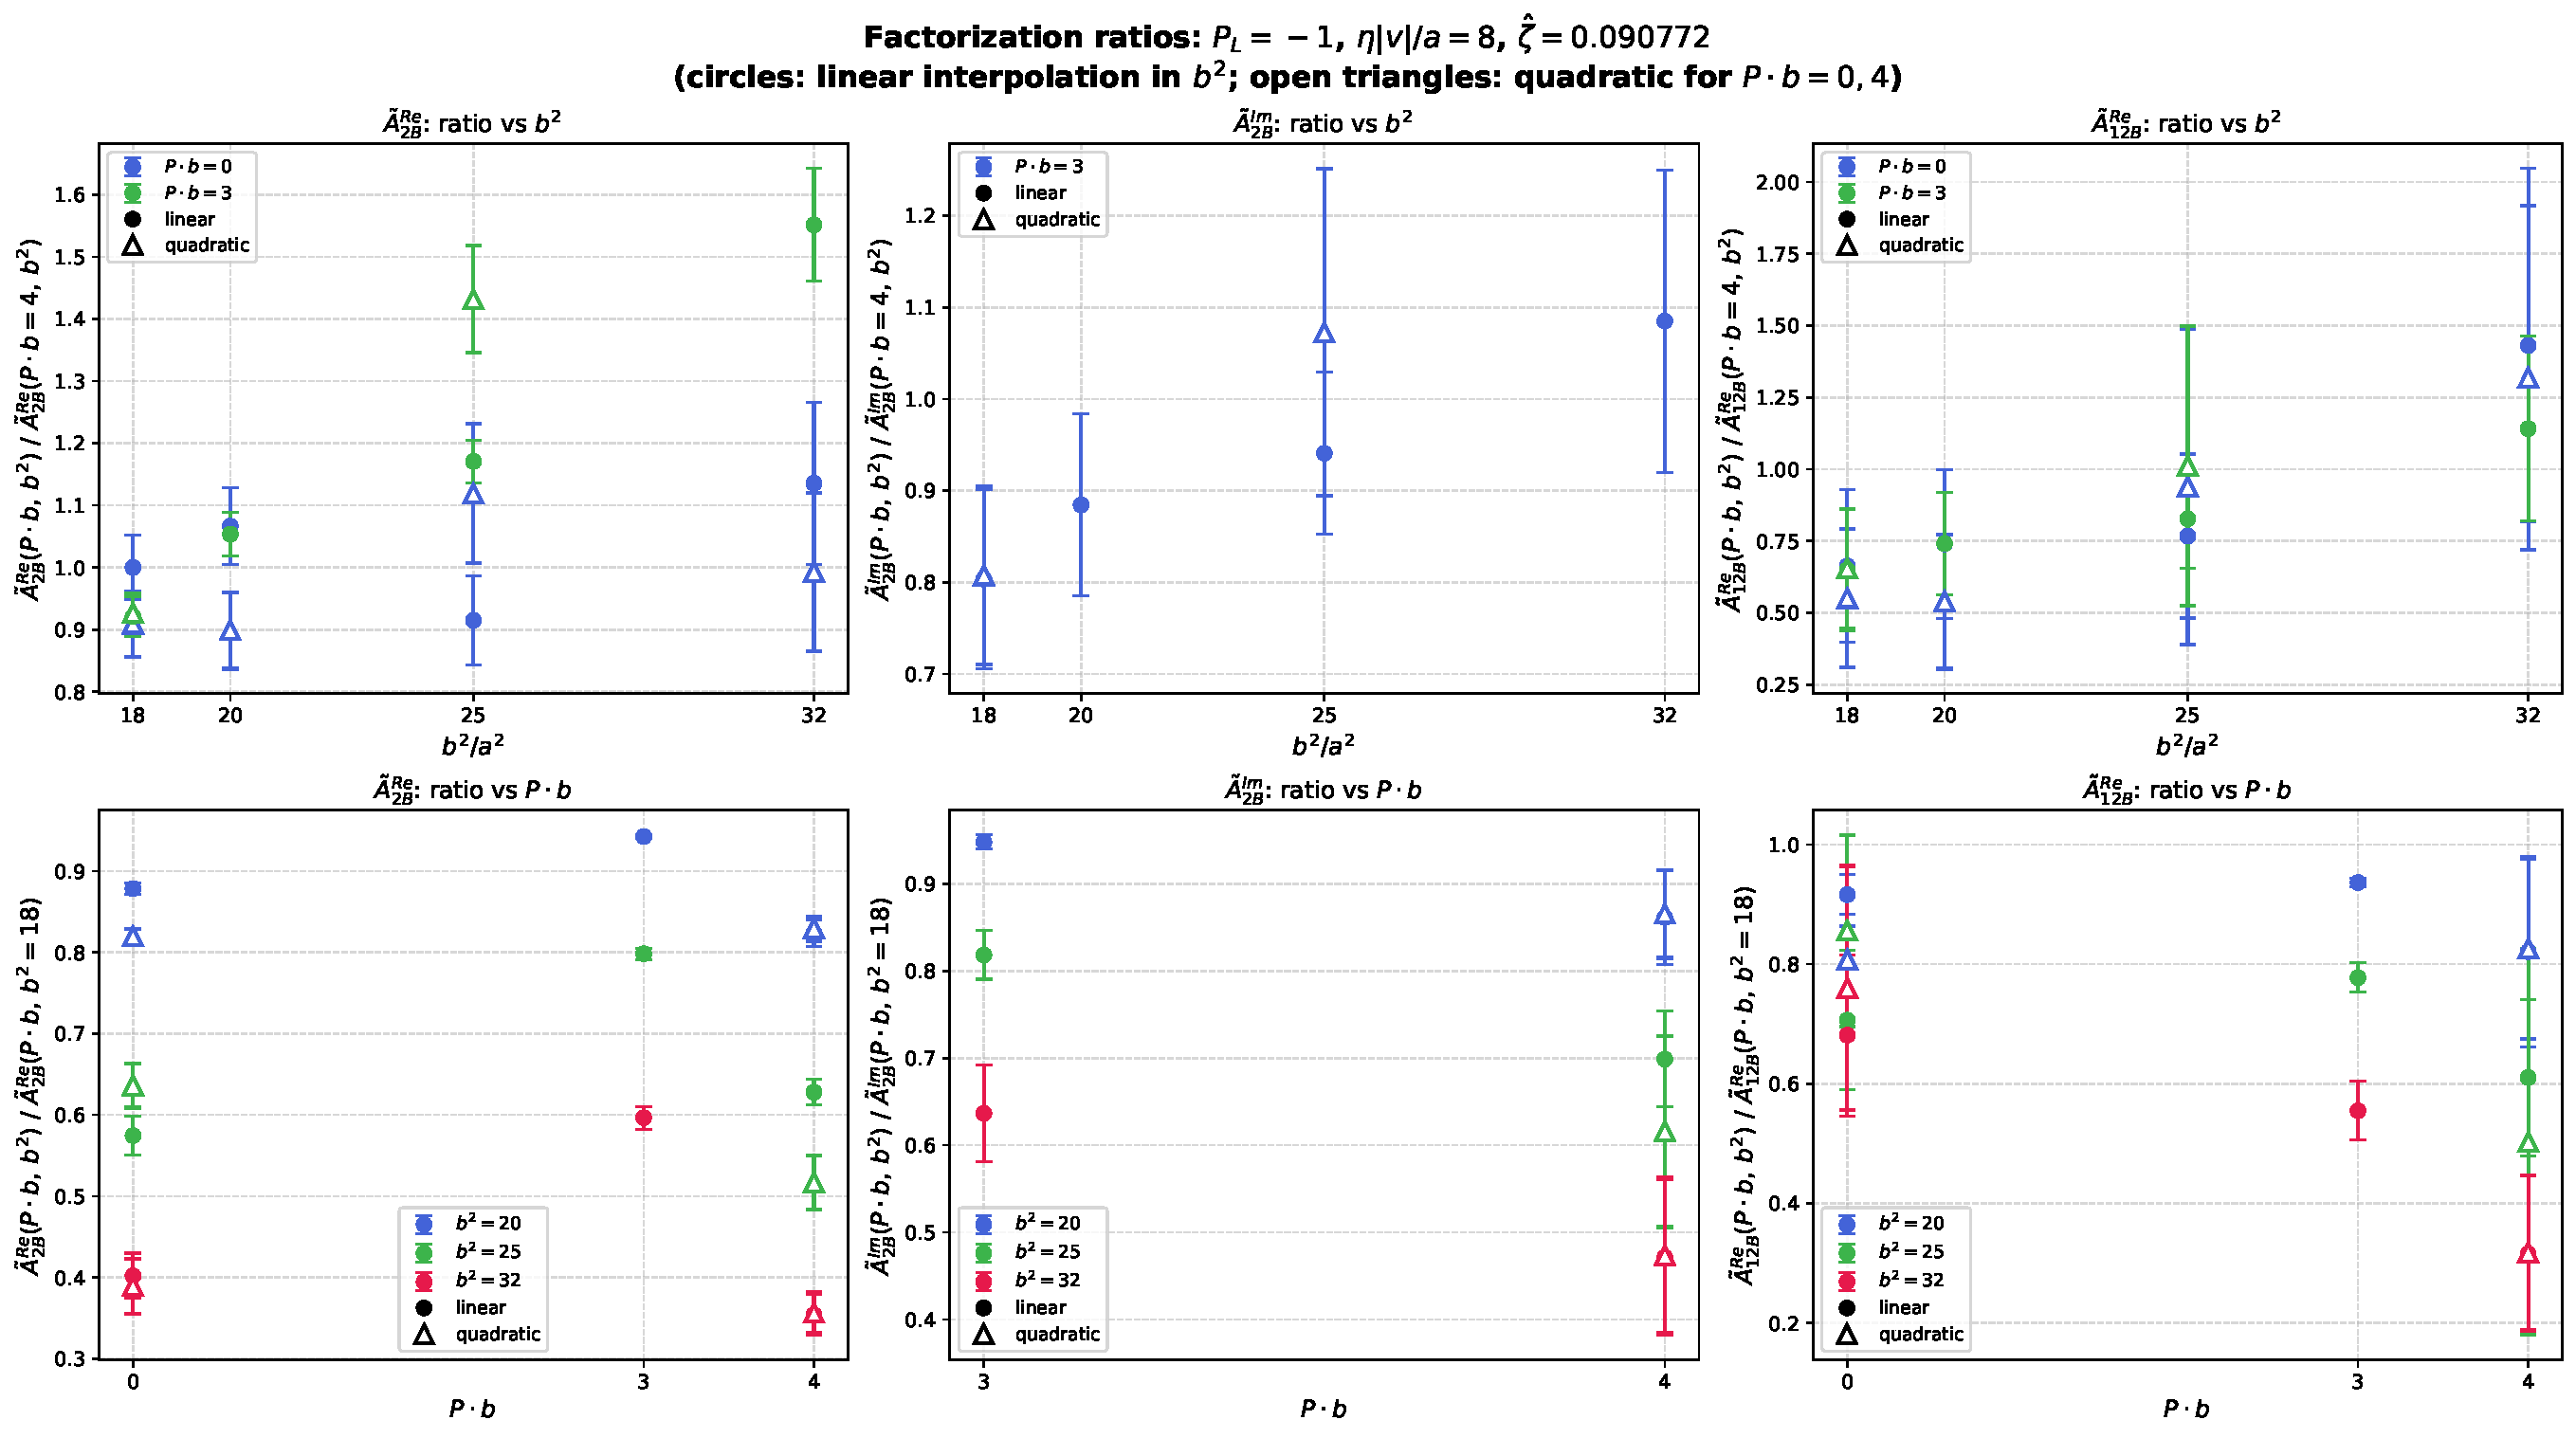
\includegraphics[width=0.8\textwidth]{figures/results/fact_ratio_data.pdf}
\caption{Factorization ratio test on the lattice data at $\eta|v|/a=8$, $P_L=-1$. Top: $T(P\cdot b,b^2)$ against $b^2$. Bottom: $B(P\cdot b,b^2)$ against $P\cdot b$. Under factorization every set of points is flat. Circles: linear interpolation in $b^2$. Triangles: quadratic interpolation on the $P\cdot b=0$ and $4$ rows. Errors are Jackknife errors and do not include the interpolation uncertainty.}
\label{fig:fact_data}
\end{figure*}

\begin{figure}
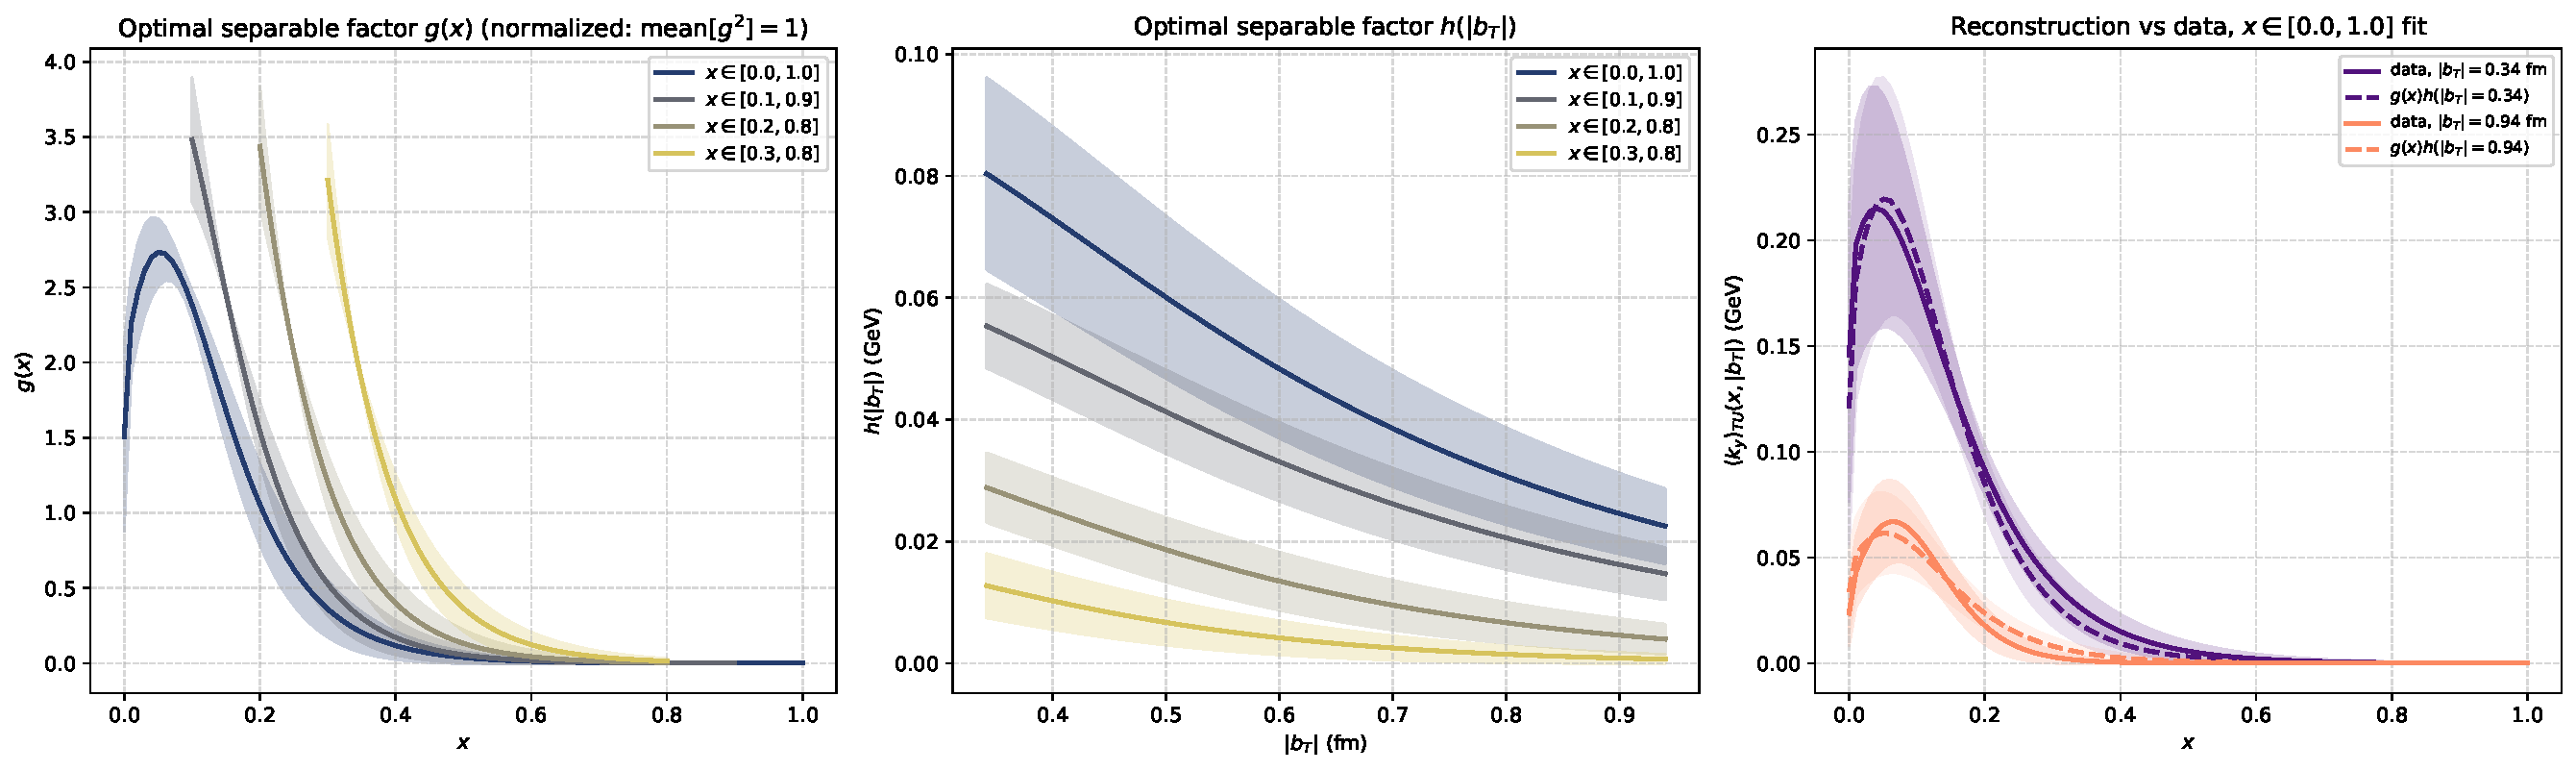
\includegraphics[width=\columnwidth]{figures/results/fact_gh_recon.pdf}
\caption{Optimal separable factors $g(x)$ and $h(|\vect b_T|)$ for the four $x$-windows of Table~\ref{tab:fact_sivers} (left, center) and the reconstruction $g\,h$ (dashed) against the extrapolated Sivers shift (solid) at the smallest and largest $|\vect b_T|$ (right).}
\label{fig:fact_gh}
\end{figure}

\begin{figure}
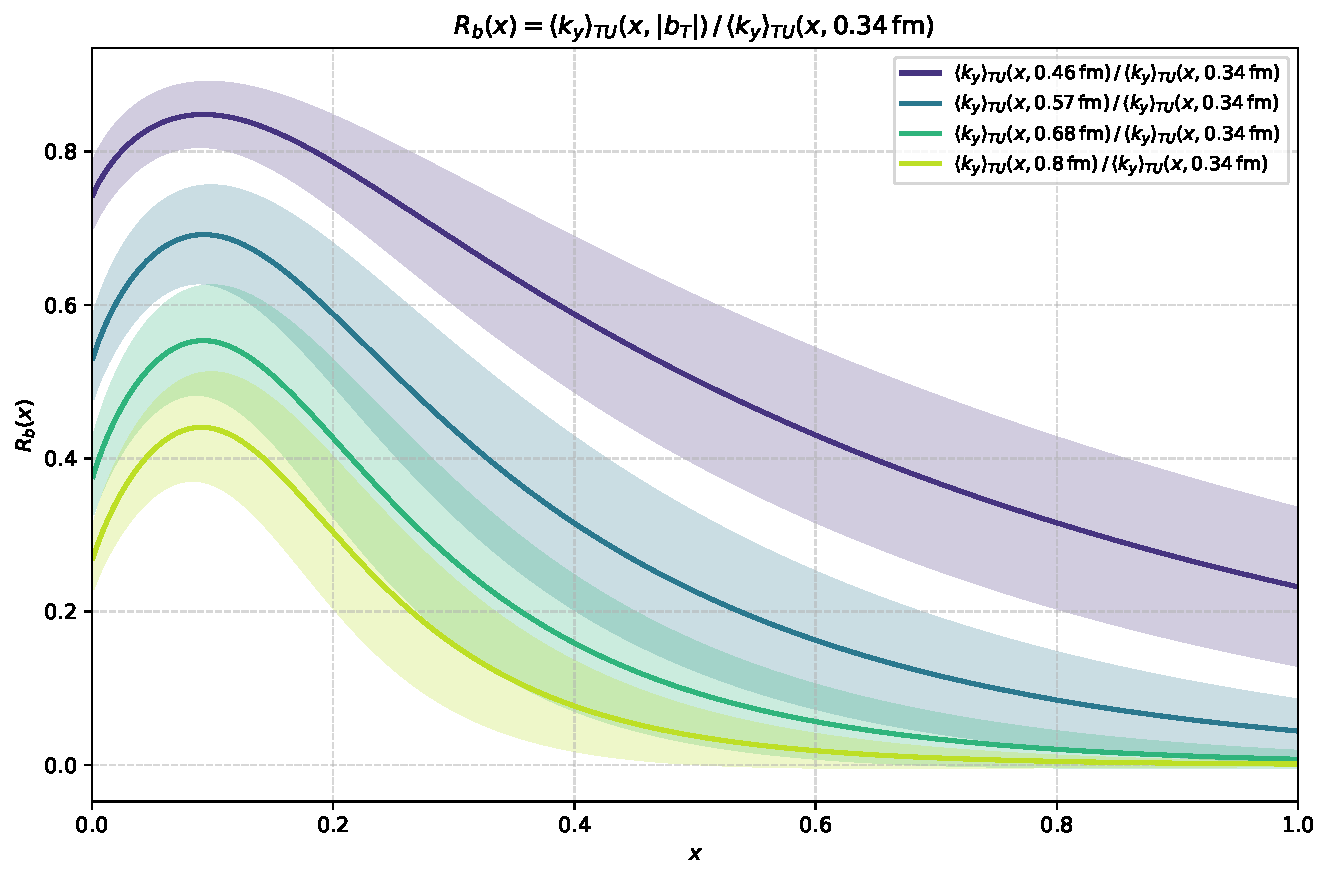
\includegraphics[width=\columnwidth]{figures/results/fact_ratio_x.pdf}
\caption{$R_b(x)$ with $|\vect b_T|_{\rm ref}=0.34$~fm for four values of $|\vect b_T|$. Each curve rises from its $x\to0$ value to a peak near $x\approx0.1$ and then decays instead of staying flat.}
\label{fig:fact_ratio_x}
\end{figure}

\begin{figure}
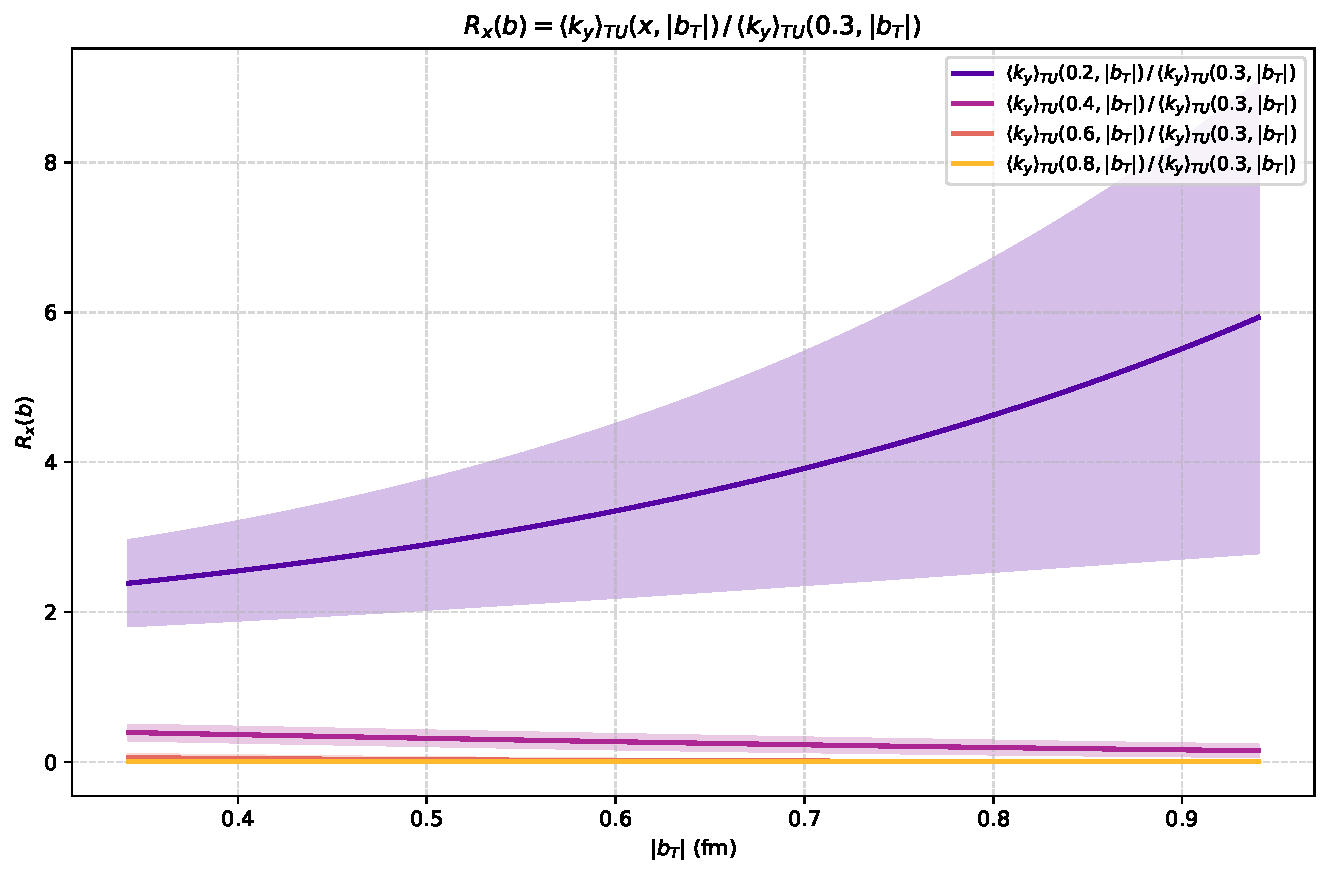
\includegraphics[width=\columnwidth]{figures/results/fact_ratio_bT.pdf}
\caption{$R_x(|\vect b_T|)$ with $x_{\rm ref}=0.3$ for four values of $x$. The $x=0.2$ curve changes by more than a factor of two across the fitted range.}
\label{fig:fact_ratio_bT}
\end{figure}


\section{Conclusions}
\label{sec:conclusions}

We have computed the dependence of the isovector ($u-d$) generalized Sivers shift on the quark longitudinal momentum fraction $x$ and on $|\vect{b}_T|$ in lattice QCD, at four nucleon momenta corresponding to $\hat\zeta=0.090772$ to $0.785756$, and extrapolated it to the light-cone limit $\hat\zeta\to\infty$. The $x$ dependence comes from a Fourier transform over $b\cdot P$ of the Lorentz-invariant amplitudes $\tAmp_{2B}$ and $\tAmp_{12B}$. In the ratio that defines the shift, the soft factor and the multiplicative, $\Gamma$-independent renormalization cancel. The invariants $v\cdot b$ and $b\cdot P$ are tied together, and we satisfy this constraint over a continuous range of $b\cdot P$ by taking $\vprp{v}\perp\vprp{b}$ and by interpolating between lattice paths to reach off-axis staple directions.

A global power-law fit in $(b\cdot P,b^2,\eta)$ for $|\vect{b}|\ge3a$, guided by symbolic regression, describes the amplitudes, while a Gaussian profile and separable exponential forms fail. At $|\vect{b}_T|=0.34$~fm, $\langle k_y\rangle_{TU}$ peaks at about $0.21$~GeV at small $x$ and falls to near zero by $x\approx0.5$, and $x\langle k_y\rangle_{TU}$ peaks at about $0.02$~GeV near $x\approx0.15$. The overall sign reverses between the SIDIS and DY limits while the magnitude is unchanged. For $0.34\le|\vect{b}_T|\le0.94$~fm, the shift is factorized as $F(x)G(|\vect{b}_T|)$ to within about $5.7$--$7.6\%$ in the relative $L_2$ sense, which makes a factorized form a good but not exact approximation. The residual traces back to the extrapolated fit parameters of the three amplitudes, which differ more than their uncertainties allow.

Several limitations apply. The $\hat\zeta\to\infty$ extrapolation uses three momenta, the results are for a single ensemble with $a=0.11403$~fm and $m_\pi=317$~MeV, and the imaginary Sivers amplitude was dropped because it is consistent with zero. Only the Sivers-shift ratio is a physical quantity, since the individual amplitudes are unrenormalized.

The same method applies to the other leading-twist TMDs from the Dirac structures $\gamma^+\gamma_5$ and $i\sigma^{i+}\gamma_5$, such as the generalized Boer-Mulders shift, the worm-gear shift $\langle k_x\rangle_{TL}$ and the $x$-dependent generalized tensor charge, whose $x$-integrated versions were computed in Refs.~\cite{Musch:2011er,Musch:2010ka}. Their $x$ dependence has not yet been studied.

\begin{acknowledgments}
We thank Matthew Sievert for helpful discussions on TMDs and Andrew Dotson for help with setting up PySR. This work was supported by the U.S. Department of Energy, Office of Science, Office of Nuclear Physics, under Award Numbers DE-FG02-96ER40965 and DE-SC0024644 (the EXCLAIM Collaboration). This research used resources of the National Energy Research Scientific Computing Center (NERSC), a U.S. Department of Energy Office of Science User Facility located at Lawrence Berkeley National Laboratory. We used the Wolfram Mathematica license provided by the Department of Physics at NMSU.
% TODO(Hari): confirm acknowledgment wording and the ensemble-provider acknowledgment (JLab/W&M collaboration) required by the journal.
\end{acknowledgments}

\appendix
\begin{widetext}
\section{Symmetry constraints and amplitude parametrization}
\label{app:symmetries}
\subsection{Symmetry constraints}
Discrete symmetries constrain the correlation function. Consider the unsubtracted correlator~\cite{Boer:2011xd}:
\begin{align}
  \Phi^{[\GammaOp]}_{\text{unsub}} (\kei,P,S;v,\mu) & = \int \frac{d^4 \elll}{(2\pi)^4} \ 
  e^{i\kei \cdot \elll} 
  \underbrace{ \frac{1}{2} \bra{\nucl{P,S}}\ \bar \quark(0)\ \overbrace{ \mathcal{U}[0,\infty v]\ \mathcal{U}[\infty v,\elll] }^{\displaystyle \U} \GammaOp\ \quark(\elll)\ \ket{\nucl{P,S}} }_{\displaystyle \widetilde \Phi^{[\GammaOp]}_{\text{unsub}}(\elll,P,S;v,\mu) }\ .
  \label{eq-corrunmod}
\end{align}
For unpolarized quarks ($\Gamma = \gamma^\mu$), its decomposition into real-valued Lorentz-invariant amplitudes reads
\begin{align}
\frac{1}{2} \Phi^{[\gamma^\mu]}_{\text{unsub}} & = P^\mu\, \Amp_2 +\kei^\mu\, \Amp_3 + \frac{1}{\mN} \epsilon^{\mu \nu \alpha \beta} P_\nu \kei_\alpha S_\beta\, \Amp_{12} + \frac{\mN^2}{(v \tcdot P)} v^\mu\, \Bmp_1 \nonumber\\
& + \frac{\mN}{v \tcdot P} \epsilon^{\mu \nu \alpha \beta} P_\nu v_\alpha S_\beta\, \Bmp_7 + \frac{ \mN}{v \tcdot P} \epsilon^{\mu \nu \alpha \beta} \kei_\nu v_\alpha S_\beta\, \Bmp_8 \nonumber\\ 
& + \frac{1}{\mN (v \tcdot P)} (\kei \tcdot S) \epsilon^{\mu \nu \alpha \beta} P_\nu \kei_\alpha v_\beta\, \Bmp_9  + \frac{\mN}{(v \tcdot P)^2} (v \tcdot S) \epsilon^{\mu \nu \alpha \beta} P_\nu \kei_\alpha v_\beta \Bmp_{10}\ . 
\label{eq-phidecomp}
\end{align}
On applying Lorentz transformations ($L$), parity transformation ($P$), time-reversal ($T$), and Hermitian conjugation ($\dagger$) to the matrix elements, we find that the correlator fulfills~\cite{Musch:2011er, Boer:2011xd}:
\begin{align}
	&(L): &\Phi^{[\Gamma]}_{\text{unsub}}(k,P,S;v,\mu)  
	&= \Phi^{[\Lambda_{1/2}^{-1}\Gamma\Lambda_{1/2}^{\phantom{-1}}]}_{\text{unsub}}(\Lambda k,\Lambda P, \Lambda S;\Lambda v,\mu) \ ,\label{eq-lortrans} \displaybreak[0] \\
	&(P): &\Phi^{[\Gamma]}_{\text{unsub}}(k,P,S;v,\mu)  
	&= \Phi^{[\gamma^0\Gamma\gamma^0]}_{\text{unsub}}(\overline{k},\overline{P},-\overline{S};\overline{v},\mu) \ ,\label{eq-conpar} \displaybreak[0] \\
	&(T): &\left[ \Phi^{[\Gamma]}_{\text{unsub}}(k,P,S;v,\mu) \right]^* &= \Phi^{[\gamma^1 \gamma^3 \Gamma^* \gamma^3 \gamma^1]}_{\text{unsub}}(\overline{k},\overline{P},\overline{S};-\overline{v},\mu) \ , \label{eq-contime} \displaybreak[0] \\
	&(\dagger): &\left[  \Phi^{[\Gamma]}_{\text{unsub}}(k,P,S;v,\mu) \right]^* &= \Phi^{[\gamma^0 \Gamma^\dagger \gamma^0]}_{\text{unsub}}(k,P,S;v,\mu) \ . \label{eq-conherm}
\end{align}
where, for a vector $c$, $\overline{c} \equiv (c^0, -c^1, -c^2, -c^3)$ denotes the vector with its spatial components reversed in sign. Hermiticity $(\dagger)$ implies that the $\Amp_i$ and $\Bmp_i$ in Eq.\ \eqref{eq-phidecomp} are real valued. Time reversal $(T)$ does not constrain the number of allowed structures, because it changes the sign of $(v\cdot P)$. Instead, time reversal $(T)$ relates the SIDIS amplitudes $A_i^{(+)}$, $B_i^{(+)}$ to the Drell-Yan amplitudes $A_i^{(-)}$, $B_i^{(-)}$.
	
For any of the transformations $\mathcal{T} \in \{ L, P, T, \dagger \}$, the Eqs.\ \eqref{eq-lortrans}-\eqref{eq-conherm} are of the general form 
\begin{equation}
	\mathcal{T}_\Phi\left(\Phi(\kei,w)\right) = \Phi\left(\mathcal{T}_\kei(\kei),\mathcal{T}_w(w)\right)
\end{equation}
where we omit the subscript ``unsub'' and the renormalization scale $\mu$, and the symbol $w$ collects all dependence on $\GammaOp$, $P$, $S$ and $v$. Here $\mathcal{T}_\Phi$ is either the identity function or complex conjugation. The transformation rule $\mathcal{T}_\kei(\kei)$ maps onto $\Lambda \kei$, $\kei$ or $\overline{\kei}$ and thus fulfills $a \tcdot b = \mathcal{T}_\kei(a) \tcdot \mathcal{T}_\kei(b)$ for any two vectors $a$ and $b$. The Fourier-transformed correlator 
\begin{equation}
	\widetilde{\Phi}(\elll,w) =  \int d^4 \kei \ e^{-i \kei \tcdot \elll} \Phi(\kei, w)
\end{equation}
transforms according to
\begin{align}
	\mathcal{T}_\Phi\left(\widetilde{\Phi}(\elll,w) \right) & =  \int d^4 \kei \ e^{\mathcal{T}_\Phi(-i)\, \kei \tcdot \elll}\ \mathcal{T}_\Phi \left( \Phi(\kei, w) \right) \nonumber \\
	& =  \int d^4 q \ e^{\mathcal{T}_\Phi(-i)\, \mathcal{T}^{-1}_\kei(q) \tcdot \elll} \ \Phi\left(q, \mathcal{T}_w( w) \right) \nonumber \\
	& \qquad\qquad \text{(change of variables: $\kei\rightarrow q=\mathcal{T}_\kei(\kei)$, i.e.\ $\kei=\mathcal{T}^{-1}_\kei(q)$)}  \nonumber \\
	& =  \int d^4 q \ e^{\mathcal{T}_\Phi(-i)\, q \tcdot \mathcal{T}_\kei(\elll)} \ \Phi\left(q, \mathcal{T}_w( w) \right) \qquad (\because q \tcdot b = \mathcal{T}_\kei(q) \tcdot \mathcal{T}_\kei(b)) \nonumber \\
    & =  \int d^4 q \ e^{-iq\left(\frac{\mathcal{T}_\Phi(i)}{i}\,  \tcdot \mathcal{T}_\kei(\elll)\right)} \ \Phi\left(q, \mathcal{T}_w( w) \right)\nonumber \\
	& = \widetilde{\Phi}\left( \frac{\mathcal{T}_\Phi(i)}{i} \mathcal{T}_\kei(\elll), \mathcal{T}_w(w) \right)\, .
	\label{eq-phitildetrafo}
\end{align}

In particular, under Hermitian conjugation the position-space correlator transforms as
\begin{align}
	&(\dagger): &\left[ \widetilde{\Phi}^{[\GammaOp]}_{\text{unsub}}(\elll,P,S;v)  \right]^* &= \widetilde{\Phi}^{[\gamma^0 \GammaOp^\dagger \gamma^0]}_{\text{unsub}}(-\elll,P,S;v)  \ .\label{eq-conhermtilde}
\end{align}
Let $f(\kei,w)$ be any of the structures preceding the invariant amplitudes in the parameterization of $\Phi$.
The structure $f(\kei,w)$ is a homogeneous function of some degree $n$ in $\kei$, i.e., $f(\alpha \kei,w) = \alpha^n f(\kei,w)$ for any number $\alpha$. 
For example, the structure $f(\kei,w) = \frac{1}{\mN (v \tcdot P)} (\kei \tcdot S) \epsilon^{\mu \nu \alpha \beta} P_\nu \kei_\alpha v_\beta$ preceding $\Bmp_9$ in Eq.\ \eqref{eq-phidecomp} has degree $n=2$.
If we define $\tilde f(\elll,w) \equiv f(- i \mN^2 \elll,w)$, then 
\begin{align}
	\mathcal{T}_\Phi\left( \tilde f(\elll, w) \right) =
	\mathcal{T}_\Phi(-i \mN^2)^n\, \mathcal{T}_\Phi\left( f( \elll, w) \right) =
	f\left( \mathcal{T}_\Phi(-i \mN^2) \mathcal{T}_\kei(\elll) , \mathcal{T}_w(w) \right) =
	\tilde f \left(  \frac{\mathcal{T}_\Phi(i)}{i} \elll, w \right)\, .
	\end{align}
This shows that $\tilde f$ transforms like $\widetilde \Phi$ in Eq.\ \eqref{eq-phitildetrafo}.
The parameterization of $\widetilde{\Phi}$ therefore follows from the substitution $\kei \rightarrow -i \mN^2 \elll$ in the structures parameterizing $\Phi$, which gives
\begin{align}  \frac{1}{2}\widetilde \Phi^{[\gamma^\mu]}_{\text{unsub}}  = & P^\mu\, \tAmp_2 - i \mN^2 \elll^\mu\, \tAmp_3 - i \mN \epsilon^{\mu \nu \alpha \beta} P_\nu \elll_\alpha S_\beta\, \tAmp_{12} + \frac{\mN^2}{(v \tcdot P)} v^\mu\, \tBmp_1\nonumber\\
& + \frac{\mN}{v \tcdot P} \epsilon^{\mu \nu \alpha \beta} P_\nu v_\alpha S_\beta\, \tBmp_7  - \frac{ i \mN^3}{v \tcdot P} \epsilon^{\mu \nu \alpha \beta} \elll_\nu v_\alpha S_\beta\, \tBmp_8 \nonumber\\
& - \frac{\mN^3}{v \tcdot P} (\elll \tcdot S) \epsilon^{\mu \nu \alpha \beta} P_\nu \elll_\alpha v_\beta\, \tBmp_9  - \frac{i \mN^3}{(v \tcdot P)^2} (v \tcdot S) \epsilon^{\mu \nu \alpha \beta} P_\nu \elll_\alpha v_\beta \tBmp_{10}\ . 
\label{eq-phitildedecomp}
\end{align}

The amplitudes $\tAmp_i$ and $\tBmp_i$ introduced this way are no longer constrained to be real-valued functions. Instead, Hermitian conjugation, Eq.\ \eqref{eq-conhermtilde}, gives the relation
\begin{equation}
	\left[ \tAmp_i(\elll^2,\elll \tcdot P, v \tcdot \elll / (v \tcdot P), \zeta^{-2},\mu^2) \right]^* = \tAmp_i(\elll^2,-\elll \tcdot P, -v \tcdot \elll / (v \tcdot P), \zeta^{-2},\mu^2)\, .\label{conditi_hermitian}
\end{equation}
In general, the amplitudes are complex,
\begin{align}
    \tAmp_i&=\tAmp_i^{\text{Re}}+i\tAmp_i^{\text{Im}}\\
    \tBmp_i&=\tBmp_i^{\text{Re}}+i\tBmp_i^{\text{Im}}
\end{align}
Given the amplitudes at both $\pm b$, Eq.\ \eqref{conditi_hermitian} implies
\begin{subequations}
\label{eq-ReIm-parity}
\begin{align}
    \tAmp_i^{\text{Re}}&=\tAmp_i^{\text{(b-even)}}\\
    \tAmp_i^{\text{Im}}&=\tAmp_i^{\text{(b-odd)}}\\
    \tBmp_i^{\text{Re}}&=\tBmp_i^{\text{(b-even)}}\\
    \tBmp_i^{\text{Im}}&=\tBmp_i^{\text{(b-odd)}}
\end{align}
\end{subequations}
\subsection{Correlator parametrization}
\label{sec-parametr}
To translate Euclidean space lattice calculations into TMDs, which are defined and interpreted in light cone coordinates, we need the parametrization of the correlator $\tilde \Phi_\unsub$ in terms of manifestly Lorentz-invariant amplitudes. A parametrization of the correlator 
$\Phi_\unsub(\kei,P,S;\infty v,\mu)$
for link paths that extend to infinity in a direction $v$
has been worked out in Ref.~\cite{Goeke:2005hb} and involves 32 independent amplitudes $A_i$ and $B_i$ that depend on the Lorentz-invariant quantities 
$\kei^2$, $\kei \cdot P$, $\kei \tcdot v/v \tcdot P$ and $\hat \zeta$.
Appendix~\ref{app:symmetries} shows that a parametrization of the corresponding $b$-dependent correlator $\tilde \Phi_\unsub$ is of the same form as the parametrization of $\Phi_\unsub$ if we substitute $\kei \rightarrow - i \mN^2 \bvec$, which is Eq.~\eqref{eq-phitildedecomp} (for $\Gamma = \gamma^\mu$):
\begin{align}  
\frac{1}{2}\widetilde \Phi^{[\gamma^\mu]}_{\text{unsub}}  = & P^\mu\, \tAmp_2 - i \mN^2 \elll^\mu\, \tAmp_3 - i \mN \epsilon^{\mu \nu \alpha \beta} P_\nu \elll_\alpha S_\beta\, \tAmp_{12} + \frac{\mN^2}{(v \tcdot P)} v^\mu\, \tBmp_1\nonumber\\
& + \frac{\mN}{v \tcdot P} \epsilon^{\mu \nu \alpha \beta} P_\nu v_\alpha S_\beta\, \tBmp_7  - \frac{ i \mN^3}{v \tcdot P} \epsilon^{\mu \nu \alpha \beta} \elll_\nu v_\alpha S_\beta\, \tBmp_8 \nonumber\\
& - \frac{\mN^3}{v \tcdot P} (\elll \tcdot S) \epsilon^{\mu \nu \alpha \beta} P_\nu \elll_\alpha v_\beta\, \tBmp_9  - \frac{i \mN^3}{(v \tcdot P)^2} (v \tcdot S) \epsilon^{\mu \nu \alpha \beta} P_\nu \elll_\alpha v_\beta \tBmp_{10}\ . 
\label{eq-phitildedecomp-again}
\end{align}
For the lattice calculations, it is advantageous to start with an equivalent parametrization in which the structures explicitly depend on the staple extent $\eta$ and which is still well-defined for $v \tcdot P = 0$. Such a parametrization can be obtained from the parametrization above by replacing $v \rightarrow \eta v$ and by leaving out the factors $(v \tcdot P)^{-n}$.
\begin{align}  
\frac{1}{2}\widetilde \Phi^{[\gamma^\mu]}_{\text{unsub}}  = & P^\mu\, \tilde a_2 - i \mN^2 \bvec^\mu\, \tilde a_3
		- i \mN \epsilon^{\mu \nu \alpha \beta} P_\nu \bvec_\alpha S_\beta\, \tilde a_{12} \nonumber \\ &
		~~+ \mN^2 \eta v^\mu\, \tilde b_1 
		+ \mN \epsilon^{\mu \nu \alpha \beta} P_\nu \eta v_\alpha S_\beta\, \tilde b_7  
		-  i \mN^3 \epsilon^{\mu \nu \alpha \beta} \bvec_\nu \eta v_\alpha S_\beta\, \tilde b_8 \nonumber \\ &
		~~- \mN^3 (\bvec \tcdot S) \epsilon^{\mu \nu \alpha \beta} P_\nu \bvec_\alpha \eta v_\beta\, \tilde b_9
		-i \mN^3 (v \tcdot S) \epsilon^{\mu \nu \alpha \beta} P_\nu \bvec_\alpha \eta^2 v_\beta \tilde b_{10}
\label{eq-phitildedecomp-lowere}
\end{align}
Here we have used lowercase amplitudes to distinguish the two parametrizations. The relation to the uppercase amplitudes is given by
\begin{align}
	\tAmp_i\left(\bvec^2,\bvec \tcdot P,\frac{v \tcdot \bvec}{v \tcdot P}, \frac{v^2}{(v \tcdot P)^2}, \eta v \tcdot P\right) & = \tilde a_i(\bvec^2,\bvec \tcdot P, \eta v \tcdot b, (\eta v)^2, \eta v \tcdot P)   \, , \nonumber \\
	 \tBmp_i\left(\bvec^2,\bvec \tcdot P,\frac{v \tcdot \bvec}{v \tcdot P}, \frac{v^2}{(v \tcdot P)^2}, \eta v \tcdot P\right) & = (\eta v \tcdot P)^n\ \tilde b_i(\bvec^2,\bvec \tcdot P, \eta v \tcdot b, (\eta v)^2, \eta v \tcdot P)   \, .
	\label{eq-ab}
\end{align}
where $n$ is the power with which $v \tcdot P$ appears in the denominator in front of the corresponding amplitude $\tBmp_i$ in the parametrization. 
Notice that the $\tilde a_i$ and $\tilde b_i$ are functions of all the Lorentz-invariant products of $\bvec$, $P$ and $\eta v$.
For the uppercase amplitudes, however, we choose to represent the dependence on these invariants in the third and fourth arguments by $\eta$-independent expressions, to facilitate taking the limit $\eta \rightarrow \pm \infty$. 
The dependence on the Collins-Soper parameter $\hat\zeta$ is given by the fourth argument, $v^2/(v \tcdot P)^2 = - 1 /(\mN\hat\zeta)^2$, 
while the fifth argument, $\eta v \tcdot P$, characterizes the length of the gauge link and distinguishes between future- and past-pointing
Wilson lines. 
The TMDs follow from the amplitudes through the Fourier integration operator $\fourint$,
\begin{align}
	\fourint \tAmp_i \equiv \int \frac{d^2 \vprp{\bvec}}{(2\pi)^2}\,e^{-i\vprp{\bvec}\tcdot\vprp{\kei}}\, \tAmp^{[x]}_i(x,\vprp{\bvec}^2)\,, \label{eq-fourint} \\
	\tAmp^{[x]}_i(x,\vprp{\bvec}^2) \equiv \frac{1}{\widetilde{\mathcal{S}}(\bvec^2;\ldots)} \int_{-\infty}^{\infty} \frac{d(\bvec \tcdot P)}{2\pi}\, e^{ix(\bvec \tcdot P)}\, \tAmp_{i}\big(\bvec^2,\bvec \tcdot P,\ldots\big)\,, \nonumber
\end{align}
and, applied to the combined amplitudes of Eq.~\eqref{eq-ABamps_sivers},
\begin{align}
	f_1(x,\vprp{\kei}^2;\zetahat,\ldots,\eta v \tcdot P) & = 2 \fourint\ \tAmp_{2B} \,,\nonumber \\
	f_{1T}^\perp(x,\vprp{\kei}^2;\zetahat,\ldots,\eta v \tcdot P) & =  4 m_N^2 \partial_{\vprp{\kei}^2} \fourint\ \tAmp_{12B} \ .
	\label{eq-tmdsfromampsodd}
\end{align}
Eq.~\eqref{eq-fourint} gives $\fourint \tAmp_i = \int \frac{d^2 \vprp{\bvec}'}{(2\pi)^2}\, e^{-i\vprp{\bvec}'\tcdot\vprp{\kei}}\, \tAmp^{[x]}_i(x,\vprp{\bvec}'^2)$. Inserting $f_1 = 2\fourint\tAmp_{2B}$ into Eq.~\eqref{eq-FTMD}, we have for the unpolarized TMD,
\begin{align}
	\tilde f_1(x,\vprp{\bvec}^2) 
	&= 2 \int d^2\vprp{\kei}\, e^{i\vprp{\bvec}\tcdot\vprp{\kei}} \int \frac{d^2 \vprp{\bvec}'}{(2\pi)^2}\, e^{-i\vprp{\bvec}'\tcdot\vprp{\kei}}\, \tAmp^{[x]}_{2B}(x,\vprp{\bvec}'^2) 
	= 2 \int d^2 \vprp{\bvec}'\, \delta^{(2)}(\vprp{\bvec}-\vprp{\bvec}')\, \tAmp^{[x]}_{2B}(x,\vprp{\bvec}'^2) \nonumber\\
	&= 2\, \tAmp^{[x]}_{2B}(x,\vprp{\bvec}^2)\,,
\end{align}
For Sivers TMD, on starting from $f_{1T}^\perp = 4\mN^2\,\partial_{\vprp{\kei}^2}\fourint\tAmp_{12B}$ and using $\vect{k}_j\,\partial_{\vprp{\kei}^2} = \tfrac12\,\partial_{\vect{k}_j}$, differentiating Eq.~\eqref{eq-FTMD} with respect to $\vect{b}_j$, we have
\begin{align}
	\partial_{\vect{b}_j}\tilde f_{1T}^\perp 
	&= \int d^2\vprp{\kei}\,(i\vect{k}_j)\,e^{i\vprp{\bvec}\tcdot\vprp{\kei}}\; 4\mN^2\,\partial_{\vprp{\kei}^2}\fourint\tAmp_{12B}
	 = 2i\mN^2 \int d^2\vprp{\kei}\, e^{i\vprp{\bvec}\tcdot\vprp{\kei}}\;\partial_{\vect{k}_j}\fourint\tAmp_{12B} \nonumber\\
	&= -2i\mN^2\,(i\vect{b}_j) \int d^2\vprp{\kei}\, e^{i\vprp{\bvec}\tcdot\vprp{\kei}}\,\fourint\tAmp_{12B}
	 = 2\mN^2\,\vect{b}_j\,\tAmp^{[x]}_{12B}(x,\vprp{\bvec}^2)\,,
\end{align}
where we integrated by parts in $\vect{k}_j$ (the surface term vanishes for $|\vprp{\bvec}|>0$) and used the same $\delta$-function step as for $f_1$. Since $\partial_{\vect{b}_j}\tilde f = 2\vect{b}_j\,\partial_{\vprp{\bvec}^2}\tilde f$, this gives $\partial_{\vprp{\bvec}^2}\tilde f_{1T}^\perp = \mN^2\,\tAmp^{[x]}_{12B}$. Eq.~\eqref{eq-dFTMD} with $n=1$ then yields
\begin{equation}
	\tilde f_{1T}^{\perp(1)}(x,\vprp{\bvec}^2) = -\frac{2}{\mN^2}\,\partial_{\vprp{\bvec}^2}\tilde f_{1T}^\perp(x,\vprp{\bvec}^2) = -2\,\tAmp^{[x]}_{12B}(x,\vprp{\bvec}^2)\,.
\end{equation}
These results establish Eqs.~\eqref{eq-xintderfttmds1} and~\eqref{eq-xintderfttmds2}.
\end{widetext}

\section{Explicit $\hat\zeta$ calculation for $P_1=-1$}
\label{app:explicit_zeta}
Setting the right-hand side of Eq. \eqref{constraints} to zero implies that the bracketed term
\begin{equation*}
\left[\frac{P_{1}}{m_{N}}\left(\hat{\zeta}-\sqrt{\hat{\zeta}^2+1}\right)+\hat{\zeta}\frac{m_{N}}{P_{1}}\right]
\end{equation*}
must vanish. This fixes the required Collins-Soper parameter, up to a sign, for a given lattice momentum. Using the lattice ensemble parameters from our lattice size of $\{\hat{L}^3\times\hat{T}\}=\{32^3\times96\}$ and lattice unit of $a=0.11403\text{ fm}$ (pion mass $m_\pi=317\text{ MeV}$), the nucleon mass and the lowest momentum mode are:
\begin{align}
    \mN &= \frac{0.6228(28)}{0.11403\text{ fm}} \nonumber \\
    &= \frac{0.6228(28)\times 197.32698 \text{ MeV}}{0.11403} \nonumber \\
    &= 1077.8(48)\text{ MeV} \ , \\
    P_{1}&=-\frac{2\pi}{L}=-\frac{2\pi}{32\times 0.11403\text{ fm}} \nonumber \\
    &=-339.8\text{ MeV} \ .
\end{align}
Substituting these values into the constraint equation yields:
\begin{align}
   \Longrightarrow \left[\frac{P_{1}}{m_{N}}\left(\hat{\zeta}-\sqrt{\hat{\zeta}^2+1}\right)+\hat{\zeta}\frac{m_{N}}{P_{1}}\right]&=0 \nonumber \\
    \Longrightarrow \hat{\zeta} &=\sqrt{\frac{P_{1}^2}{m_{N}^{2}\left(\frac{m_{N}^{2}}{P_{1}^{2}}+2\right)}} \nonumber \\
    \hat{\zeta} &= \pm 0.09077(75) \nonumber \\
    \hat{\zeta} &= \pm 0.090772 \ .
\end{align}
With $\hat{\zeta}$ determined, we can derive the specific orientation of the space-like staple vector $v$. From the definition of $\hat{\zeta}$:
\begin{align}
    \hat{\zeta}&=\frac{-v_{1}P_{1}}{|v|\mN}=\frac{-v_{1}P_{1}}{\left(\sqrt{v_{1}^{2}+0^{2}+v_{3}^{2}}\right)m_{N}} \ .
\end{align}
Solving for the longitudinal staple component $v_1$ in terms of the transverse component $v_3$:
\begin{align}
    \Longrightarrow v_{1}=\pm 0.301~v_{3} \ .
\end{align}

The same calculation for $P_1=-2,-3,-4$ gives the values in Table~\ref{tab:zeta_directions}.

\section{Gauge-link paths}
\label{app:paths}
\subsection{Staple paths}
\begin{figure}[htpb]
    \centering
    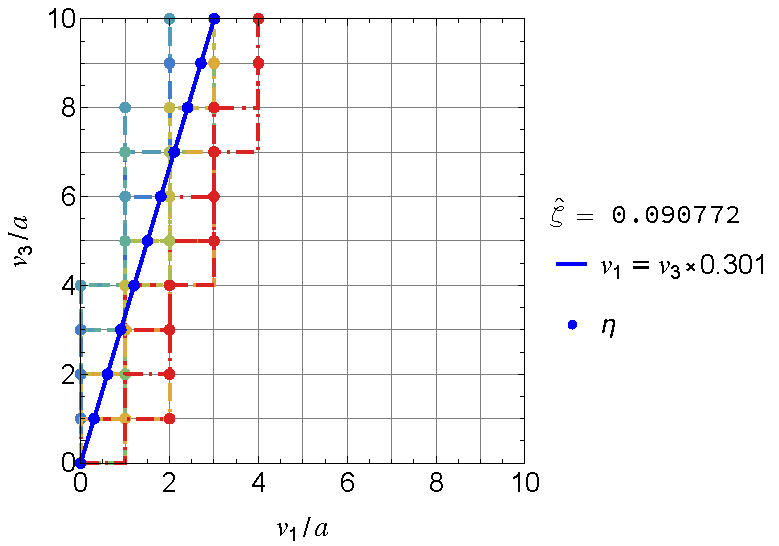
\includegraphics[width=0.6\linewidth]{figures/v1_v2_withPath_forP-1_plot.pdf}
        \caption{Ideal continuous trajectory of the off-axis staple vector (solid blue) for $P_1 = -1$. Circular markers indicate target continuous coordinates for sequential values of $\eta$. Dashed lines illustrate the discrete, step-wise permutations of gauge links used to reach the surrounding bounding integer lattice sites.}
        \label{fig:v_path_P-1}
\end{figure}

\begin{table*}[htbp]
    \centering
\begin{ruledtabular}
\begin{tabular}{ll}
$\eta\,\vect{v}/a$ & \parbox[t]{0.72\textwidth}{\raggedright Gauge-link paths for interpolation ($\hat\zeta = 0.090772$)} \\
\hline
$0\cdot(0.301,0,1)$ & \parbox[t]{0.72\textwidth}{\raggedright $\{$\mbox{$\{\}$}$\}$} \\
$1\cdot(0.301,0,1)$ & \parbox[t]{0.72\textwidth}{\raggedright $\{$\mbox{$\{3\}$}, \mbox{$\{1,3\}$}, \mbox{$\{3,1\}$}, \mbox{$\{1,3,1\}$}$\}$} \\
$2\cdot(0.301,0,1)$ & \parbox[t]{0.72\textwidth}{\raggedright $\{$\mbox{$\{3,3\}$}, \mbox{$\{3,1,3\}$}, \mbox{$\{1,3,1,3\}$}, \mbox{$\{3,1,3,1\}$}$\}$} \\
$3\cdot(0.301,0,1)$ & \parbox[t]{0.72\textwidth}{\raggedright $\{$\mbox{$\{3,3,3\}$}, \mbox{$\{3,1,3,3\}$}, \mbox{$\{3,3,1,3\}$}, \mbox{$\{3,1,3,1,3\}$}$\}$} \\
$4\cdot(0.301,0,1)$ & \parbox[t]{0.72\textwidth}{\raggedright $\{$\mbox{$\{3,3,3,3\}$}, \mbox{$\{3,3,1,3,3\}$}, \mbox{$\{3,1,3,3,1,3\}$}$\}$} \\
$5\cdot(0.301,0,1)$ & \parbox[t]{0.72\textwidth}{\raggedright $\{$\mbox{$\{3,3,1,3,3,3\}$}, \mbox{$\{3,3,3,1,3,3\}$}, \mbox{$\{3,3,1,3,1,3,3\}$}, \mbox{$\{3,1,3,1,3,3,1,3\}$}, \mbox{$\{3,1,3,3,1,3,1,3\}$}$\}$} \\
$6\cdot(0.301,0,1)$ & \parbox[t]{0.72\textwidth}{\raggedright $\{$\mbox{$\{3,3,3,1,3,3,3\}$}, \mbox{$\{3,3,1,3,3,1,3,3\}$}, \mbox{$\{3,1,3,3,1,3,3,1,3\}$}$\}$} \\
$7\cdot(0.301,0,1)$ & \parbox[t]{0.72\textwidth}{\raggedright $\{$\mbox{$\{3,3,3,1,3,3,3,3\}$}, \mbox{$\{3,3,3,3,1,3,3,3\}$}, \mbox{$\{3,3,1,3,3,3,1,3,3\}$}, \mbox{$\{3,3,1,3,1,3,3,1,3,3\}$}, \mbox{$\{3,3,1,3,3,1,3,1,3,3\}$}$\}$} \\
$8\cdot(0.301,0,1)$ & \parbox[t]{0.72\textwidth}{\raggedright $\{$\mbox{$\{3,3,3,3,1,3,3,3,3\}$}, \mbox{$\{3,3,3,1,3,3,1,3,3,3\}$}, \mbox{$\{3,3,1,3,3,1,3,3,1,3,3\}$}$\}$} \\
$9\cdot(0.301,0,1)$ & \parbox[t]{0.72\textwidth}{\raggedright $\{$\mbox{$\{3,3,3,1,3,3,3,1,3,3,3\}$}, \mbox{$\{3,3,1,3,3,1,3,3,3,1,3,3\}$}, \mbox{$\{3,3,1,3,3,3,1,3,3,1,3,3\}$}, \mbox{$\{3,3,1,3,3,1,3,1,3,3,1,3,3\}$}$\}$} \\
$10\cdot(0.301,0,1)$ & \parbox[t]{0.72\textwidth}{\raggedright $\{$\mbox{$\{3,3,3,1,3,3,3,3,1,3,3,3\}$}, \mbox{$\{3,3,1,3,3,3,1,3,3,3,1,3,3\}$}, \mbox{$\{3,3,1,3,3,1,3,3,1,3,3,1,3,3\}$}$\}$} \\
\end{tabular}
\end{ruledtabular}
        \caption{Discrete gauge link configurations defining the interpolation bounds for $P_1 = -1$. Empty brackets $\{\}$ denote a zero-length origin link, while numerical arrays (e.g., $\{1,3,1\}$) give the sequence of directional steps.}
        \label{tab:eta_table_P-1}
\end{table*}


% ---------------------------------------------------------
% P_1 = -2 Figures
% ---------------------------------------------------------
\begin{figure}[htpb]
    \centering
    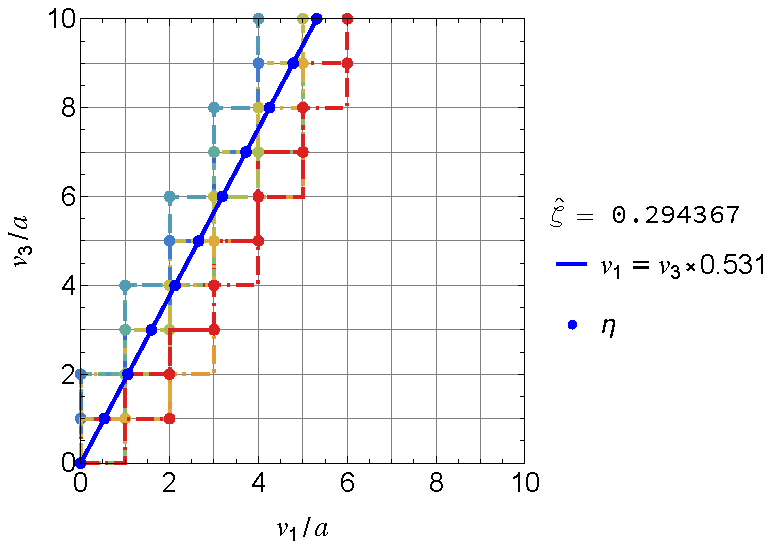
\includegraphics[width=0.6\linewidth]{figures/v1_v2_withPath_forP-2_plot.pdf}
        \caption{Ideal continuous trajectory and corresponding discrete bounding paths for the off-axis staple vector at $P_1 = -2$.}
        \label{fig:v_path_P-2}
\end{figure}

\begin{table*}[htbp]
    \centering
\begin{ruledtabular}
\begin{tabular}{ll}
$\eta\,\vect{v}/a$ & \parbox[t]{0.72\textwidth}{\raggedright Gauge-link paths for interpolation ($\hat\zeta = 0.294367$)} \\
\hline
$0\cdot(0.531,0,1)$ & \parbox[t]{0.72\textwidth}{\raggedright $\{$\mbox{$\{\}$}$\}$} \\
$1\cdot(0.531,0,1)$ & \parbox[t]{0.72\textwidth}{\raggedright $\{$\mbox{$\{3\}$}, \mbox{$\{1,3\}$}, \mbox{$\{3,1\}$}, \mbox{$\{1,3,1\}$}$\}$} \\
$2\cdot(0.531,0,1)$ & \parbox[t]{0.72\textwidth}{\raggedright $\{$\mbox{$\{3,3\}$}, \mbox{$\{3,1,3\}$}, \mbox{$\{1,3,1,3\}$}, \mbox{$\{3,1,3,1\}$}$\}$} \\
$3\cdot(0.531,0,1)$ & \parbox[t]{0.72\textwidth}{\raggedright $\{$\mbox{$\{3,1,3,3\}$}, \mbox{$\{3,3,1,3\}$}, \mbox{$\{3,1,3,1,3\}$}, \mbox{$\{1,3,1,3,1,3\}$}, \mbox{$\{3,1,3,1,3,1\}$}$\}$} \\
$4\cdot(0.531,0,1)$ & \parbox[t]{0.72\textwidth}{\raggedright $\{$\mbox{$\{3,3,1,3,3\}$}, \mbox{$\{3,1,3,3,1,3\}$}, \mbox{$\{3,1,3,1,3,1,3\}$}$\}$} \\
$5\cdot(0.531,0,1)$ & \parbox[t]{0.72\textwidth}{\raggedright $\{$\mbox{$\{3,3,1,3,1,3,3\}$}, \mbox{$\{3,1,3,1,3,3,1,3\}$}, \mbox{$\{3,1,3,3,1,3,1,3\}$}, \mbox{$\{3,1,3,1,3,1,3,1,3\}$}$\}$} \\
$6\cdot(0.531,0,1)$ & \parbox[t]{0.72\textwidth}{\raggedright $\{$\mbox{$\{3,3,1,3,3,1,3,3\}$}, \mbox{$\{3,1,3,3,1,3,3,1,3\}$}, \mbox{$\{3,1,3,1,3,3,1,3,1,3\}$}$\}$} \\
$7\cdot(0.531,0,1)$ & \parbox[t]{0.72\textwidth}{\raggedright $\{$\mbox{$\{3,3,1,3,1,3,3,1,3,3\}$}, \mbox{$\{3,3,1,3,3,1,3,1,3,3\}$}, \mbox{$\{3,1,3,3,1,3,1,3,3,1,3\}$}, \mbox{$\{3,1,3,1,3,1,3,3,1,3,1,3\}$}, \mbox{$\{3,1,3,1,3,3,1,3,1,3,1,3\}$}$\}$} \\
$8\cdot(0.531,0,1)$ & \parbox[t]{0.72\textwidth}{\raggedright $\{$\mbox{$\{3,3,1,3,3,1,3,3,1,3,3\}$}, \mbox{$\{3,1,3,3,1,3,3,1,3,3,1,3\}$}, \mbox{$\{3,1,3,3,1,3,1,3,1,3,3,1,3\}$}$\}$} \\
$9\cdot(0.531,0,1)$ & \parbox[t]{0.72\textwidth}{\raggedright $\{$\mbox{$\{3,3,1,3,3,1,3,1,3,3,1,3,3\}$}, \mbox{$\{3,1,3,3,1,3,1,3,3,1,3,1,3,3\}$}, \mbox{$\{3,3,1,3,1,3,3,1,3,1,3,3,1,3\}$}, \mbox{$\{3,1,3,1,3,3,1,3,1,3,3,1,3,1,3\}$}$\}$} \\
$10\cdot(0.531,0,1)$ & \parbox[t]{0.72\textwidth}{\raggedright $\{$\mbox{$\{3,3,1,3,3,1,3,3,1,3,3,1,3,3\}$}, \mbox{$\{3,1,3,3,1,3,3,1,3,3,1,3,3,1,3\}$}, \mbox{$\{3,1,3,3,1,3,1,3,3,1,3,1,3,3,1,3\}$}$\}$} \\
\end{tabular}
\end{ruledtabular}
        \caption{Discrete gauge link configurations defining the interpolation bounds for $P_1 = -2$.}
        \label{tab:eta_table_P-2}
\end{table*}


% ---------------------------------------------------------
% P_1 = -3 Figures
% ---------------------------------------------------------
\begin{figure}[htpb]
    \centering
    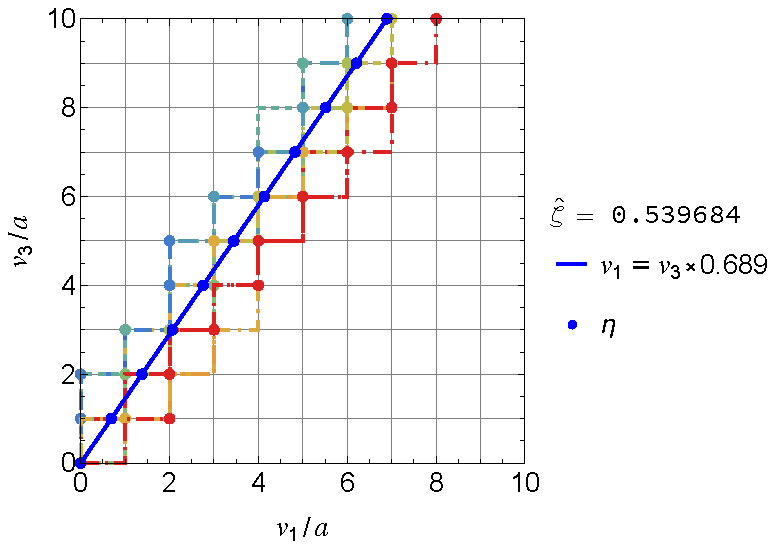
\includegraphics[width=0.6\linewidth]{figures/v1_v2_withPath_forP-3_plot.pdf}
        \caption{Ideal continuous trajectory and corresponding discrete bounding paths for the off-axis staple vector at $P_1 = -3$.}
        \label{fig:v_path_P-3}
\end{figure}

\begin{table*}[htbp]
    \centering
\begin{ruledtabular}
\begin{tabular}{ll}
$\eta\,\vect{v}/a$ & \parbox[t]{0.72\textwidth}{\raggedright Gauge-link paths for interpolation ($\hat\zeta = 0.539684$)} \\
\hline
$0\cdot(0.689,0,1)$ & \parbox[t]{0.72\textwidth}{\raggedright $\{$\mbox{$\{\}$}$\}$} \\
$1\cdot(0.689,0,1)$ & \parbox[t]{0.72\textwidth}{\raggedright $\{$\mbox{$\{3\}$}, \mbox{$\{1,3\}$}, \mbox{$\{3,1\}$}, \mbox{$\{1,3,1\}$}$\}$} \\
$2\cdot(0.689,0,1)$ & \parbox[t]{0.72\textwidth}{\raggedright $\{$\mbox{$\{3,3\}$}, \mbox{$\{3,1,3\}$}, \mbox{$\{1,3,1,3\}$}, \mbox{$\{3,1,3,1\}$}$\}$} \\
$3\cdot(0.689,0,1)$ & \parbox[t]{0.72\textwidth}{\raggedright $\{$\mbox{$\{3,1,3,3\}$}, \mbox{$\{3,3,1,3\}$}, \mbox{$\{3,1,3,1,3\}$}, \mbox{$\{1,3,1,3,1,3\}$}, \mbox{$\{3,1,3,1,3,1\}$}$\}$} \\
$4\cdot(0.689,0,1)$ & \parbox[t]{0.72\textwidth}{\raggedright $\{$\mbox{$\{3,1,3,3,1,3\}$}, \mbox{$\{3,1,3,1,3,1,3\}$}, \mbox{$\{1,3,1,3,1,3,1,3\}$}, \mbox{$\{3,1,3,1,3,1,3,1\}$}$\}$} \\
$5\cdot(0.689,0,1)$ & \parbox[t]{0.72\textwidth}{\raggedright $\{$\mbox{$\{3,3,1,3,1,3,3\}$}, \mbox{$\{3,1,3,1,3,3,1,3\}$}, \mbox{$\{3,1,3,3,1,3,1,3\}$}, \mbox{$\{3,1,3,1,3,1,3,1,3\}$}$\}$} \\
$6\cdot(0.689,0,1)$ & \parbox[t]{0.72\textwidth}{\raggedright $\{$\mbox{$\{3,1,3,3,1,3,3,1,3\}$}, \mbox{$\{3,1,3,1,3,3,1,3,1,3\}$}, \mbox{$\{3,1,3,1,3,1,3,1,3,1,3\}$}$\}$} \\
$7\cdot(0.689,0,1)$ & \parbox[t]{0.72\textwidth}{\raggedright $\{$\mbox{$\{3,1,3,3,1,3,1,3,3,1,3\}$}, \mbox{$\{3,1,3,1,3,1,3,3,1,3,1,3\}$}, \mbox{$\{3,1,3,1,3,3,1,3,1,3,1,3\}$}, \mbox{$\{3,1,3,1,3,1,3,1,3,1,3,1,3\}$}$\}$} \\
$8\cdot(0.689,0,1)$ & \parbox[t]{0.72\textwidth}{\raggedright $\{$\mbox{$\{3,1,3,3,1,3,1,3,1,3,3,1,3\}$}, \mbox{$\{3,1,3,1,3,1,3,3,1,3,1,3,1,3\}$}, \mbox{$\{3,1,3,1,3,1,3,1,3,1,3,1,3,1,3\}$}$\}$} \\
$9\cdot(0.689,0,1)$ & \parbox[t]{0.72\textwidth}{\raggedright $\{$\mbox{$\{3,1,3,3,1,3,1,3,3,1,3,1,3,3\}$}, \mbox{$\{3,3,1,3,1,3,3,1,3,1,3,3,1,3\}$}, \mbox{$\{3,1,3,1,3,3,1,3,1,3,3,1,3,1,3\}$}, \mbox{$\{3,1,3,1,3,1,3,1,3,3,1,3,1,3,1,3\}$}, \mbox{$\{3,1,3,1,3,1,3,3,1,3,1,3,1,3,1,3\}$}$\}$} \\
$10\cdot(0.689,0,1)$ & \parbox[t]{0.72\textwidth}{\raggedright $\{$\mbox{$\{3,1,3,3,1,3,1,3,3,1,3,1,3,3,1,3\}$}, \mbox{$\{3,1,3,1,3,3,1,3,1,3,1,3,3,1,3,1,3\}$}, \mbox{$\{3,1,3,1,3,1,3,1,3,3,1,3,1,3,1,3,1,3\}$}$\}$} \\
\end{tabular}
\end{ruledtabular}
        \caption{Discrete gauge link configurations defining the interpolation bounds for $P_1 = -3$.}
        \label{tab:eta_table_P-3}
\end{table*}


% ---------------------------------------------------------
% P_1 = -4 Figures
% ---------------------------------------------------------
\begin{figure}[htpb]
    \centering
    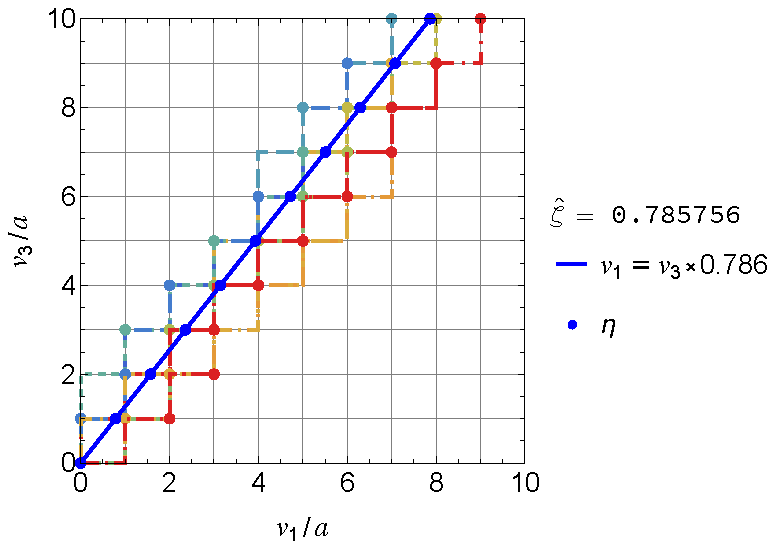
\includegraphics[width=0.6\linewidth]{figures/v1_v2_withPath_forP-4_plot.pdf}
        \caption{Ideal continuous trajectory and corresponding discrete bounding paths for the off-axis staple vector at $P_1 = -4$.}
        \label{fig:v_path_P-4}
\end{figure}

\begin{table*}[htbp]
    \centering
\begin{ruledtabular}
\begin{tabular}{ll}
$\eta\,\vect{v}/a$ & \parbox[t]{0.72\textwidth}{\raggedright Gauge-link paths for interpolation ($\hat\zeta = 0.785756$)} \\
\hline
$0\cdot(0.786,0,1)$ & \parbox[t]{0.72\textwidth}{\raggedright $\{$\mbox{$\{\}$}$\}$} \\
$1\cdot(0.786,0,1)$ & \parbox[t]{0.72\textwidth}{\raggedright $\{$\mbox{$\{3\}$}, \mbox{$\{1,3\}$}, \mbox{$\{3,1\}$}, \mbox{$\{1,3,1\}$}$\}$} \\
$2\cdot(0.786,0,1)$ & \parbox[t]{0.72\textwidth}{\raggedright $\{$\mbox{$\{3,1,3\}$}, \mbox{$\{1,3,1,3\}$}, \mbox{$\{3,1,3,1\}$}, \mbox{$\{1,3,1,3,1\}$}$\}$} \\
$3\cdot(0.786,0,1)$ & \parbox[t]{0.72\textwidth}{\raggedright $\{$\mbox{$\{3,1,3,3\}$}, \mbox{$\{3,3,1,3\}$}, \mbox{$\{3,1,3,1,3\}$}, \mbox{$\{1,3,1,3,1,3\}$}, \mbox{$\{3,1,3,1,3,1\}$}$\}$} \\
$4\cdot(0.786,0,1)$ & \parbox[t]{0.72\textwidth}{\raggedright $\{$\mbox{$\{3,1,3,3,1,3\}$}, \mbox{$\{3,1,3,1,3,1,3\}$}, \mbox{$\{1,3,1,3,1,3,1,3\}$}, \mbox{$\{3,1,3,1,3,1,3,1\}$}$\}$} \\
$5\cdot(0.786,0,1)$ & \parbox[t]{0.72\textwidth}{\raggedright $\{$\mbox{$\{3,1,3,1,3,3,1,3\}$}, \mbox{$\{3,1,3,3,1,3,1,3\}$}, \mbox{$\{3,1,3,1,3,1,3,1,3\}$}, \mbox{$\{1,3,1,3,1,3,1,3,1,3\}$}, \mbox{$\{3,1,3,1,3,1,3,1,3,1\}$}$\}$} \\
$6\cdot(0.786,0,1)$ & \parbox[t]{0.72\textwidth}{\raggedright $\{$\mbox{$\{3,1,3,1,3,3,1,3,1,3\}$}, \mbox{$\{3,1,3,1,3,1,3,1,3,1,3\}$}, \mbox{$\{1,3,1,3,1,3,1,3,1,3,1,3\}$}, \mbox{$\{3,1,3,1,3,1,3,1,3,1,3,1\}$}$\}$} \\
$7\cdot(0.786,0,1)$ & \parbox[t]{0.72\textwidth}{\raggedright $\{$\mbox{$\{3,1,3,1,3,1,3,3,1,3,1,3\}$}, \mbox{$\{3,1,3,1,3,3,1,3,1,3,1,3\}$}, \mbox{$\{3,1,3,1,3,1,3,1,3,1,3,1,3\}$}, \mbox{$\{1,3,1,3,1,3,1,3,1,3,1,3,1,3\}$}, \mbox{$\{3,1,3,1,3,1,3,1,3,1,3,1,3,1\}$}$\}$} \\
$8\cdot(0.786,0,1)$ & \parbox[t]{0.72\textwidth}{\raggedright $\{$\mbox{$\{3,1,3,3,1,3,1,3,1,3,3,1,3\}$}, \mbox{$\{3,1,3,1,3,1,3,3,1,3,1,3,1,3\}$}, \mbox{$\{3,1,3,1,3,1,3,1,3,1,3,1,3,1,3\}$}$\}$} \\
$9\cdot(0.786,0,1)$ & \parbox[t]{0.72\textwidth}{\raggedright $\{$\mbox{$\{3,1,3,1,3,3,1,3,1,3,3,1,3,1,3\}$}, \mbox{$\{3,1,3,1,3,1,3,1,3,3,1,3,1,3,1,3\}$}, \mbox{$\{3,1,3,1,3,1,3,3,1,3,1,3,1,3,1,3\}$}, \mbox{$\{3,1,3,1,3,1,3,1,3,1,3,1,3,1,3,1,3\}$}$\}$} \\
$10\cdot(0.786,0,1)$ & \parbox[t]{0.72\textwidth}{\raggedright $\{$\mbox{$\{3,1,3,1,3,3,1,3,1,3,1,3,3,1,3,1,3\}$}, \mbox{$\{3,1,3,1,3,1,3,1,3,3,1,3,1,3,1,3,1,3\}$}, \mbox{$\{3,1,3,1,3,1,3,1,3,1,3,1,3,1,3,1,3,1,3\}$}$\}$} \\
\end{tabular}
\end{ruledtabular}
        \caption{Discrete gauge link configurations defining the interpolation bounds for $P_1 = -4$.}
        \label{tab:eta_table_P-4}
\end{table*}

\subsection{Paths for the quark separation \texorpdfstring{$\vect{b}$}{b}}
\label{sec:b_gauge_links}
Constructing the direct Wilson line connecting the quark fields at $0$ and $\vect{b}$ requires generating step-wise paths across the lattice. We categorize these paths into purely transverse separations ($b_1 = 0$) and off-axis separations with a longitudinal component ($b_1 \neq 0$). For purely transverse separations, where $b \cdot P = 0$, the gauge links lie entirely within the transverse plane. Table \ref{tab:b_table_transverse} lists the link sequences used to reach these target coordinates. An empty bracket $\{\}$ denotes the local origin, while arrays such as $\{2,2\}$ indicate a sequence of two consecutive links in the $\hat{x_{2}}$-direction.

\begin{table*}[htbp]
    \centering\footnotesize
\begin{ruledtabular}
\begin{tabular}{llll}
$\{+b_1,b_2,b_3\}/a$ & \parbox[t]{0.32\textwidth}{\raggedright Gauge-link paths} & $\{-b_1,b_2,b_3\}/a$ & \parbox[t]{0.32\textwidth}{\raggedright Gauge-link paths} \\
\hline
$\{0,0,0\}$ & \parbox[t]{0.32\textwidth}{\raggedright $\{$\mbox{$\{\}$}$\}$} & $\{0,0,0\}$ & \parbox[t]{0.32\textwidth}{\raggedright $\{$\mbox{$\{\}$}$\}$} \\
$\{0,1,0\}$ & \parbox[t]{0.32\textwidth}{\raggedright $\{$\mbox{$\{2\}$}$\}$} & $\{0,1,0\}$ & \parbox[t]{0.32\textwidth}{\raggedright $\{$\mbox{$\{2\}$}$\}$} \\
$\{0,2,0\}$ & \parbox[t]{0.32\textwidth}{\raggedright $\{$\mbox{$\{2,2\}$}$\}$} & $\{0,2,0\}$ & \parbox[t]{0.32\textwidth}{\raggedright $\{$\mbox{$\{2,2\}$}$\}$} \\
$\{0,3,0\}$ & \parbox[t]{0.32\textwidth}{\raggedright $\{$\mbox{$\{2,2,2\}$}$\}$} & $\{0,3,0\}$ & \parbox[t]{0.32\textwidth}{\raggedright $\{$\mbox{$\{2,2,2\}$}$\}$} \\
$\{0,4,0\}$ & \parbox[t]{0.32\textwidth}{\raggedright $\{$\mbox{$\{2,2,2,2\}$}$\}$} & $\{0,4,0\}$ & \parbox[t]{0.32\textwidth}{\raggedright $\{$\mbox{$\{2,2,2,2\}$}$\}$} \\
$\{0,5,0\}$ & \parbox[t]{0.32\textwidth}{\raggedright $\{$\mbox{$\{2,2,2,2,2\}$}$\}$} & $\{0,5,0\}$ & \parbox[t]{0.32\textwidth}{\raggedright $\{$\mbox{$\{2,2,2,2,2\}$}$\}$} \\
$\{0,6,0\}$ & \parbox[t]{0.32\textwidth}{\raggedright $\{$\mbox{$\{2,2,2,2,2,2\}$}$\}$} & $\{0,6,0\}$ & \parbox[t]{0.32\textwidth}{\raggedright $\{$\mbox{$\{2,2,2,2,2,2\}$}$\}$} \\
$\{0,7,0\}$ & \parbox[t]{0.32\textwidth}{\raggedright $\{$\mbox{$\{2,2,2,2,2,2,2\}$}$\}$} & $\{0,7,0\}$ & \parbox[t]{0.32\textwidth}{\raggedright $\{$\mbox{$\{2,2,2,2,2,2,2\}$}$\}$} \\
$\{0,-1,0\}$ & \parbox[t]{0.32\textwidth}{\raggedright $\{$\mbox{$\{-2\}$}$\}$} & $\{0,-1,0\}$ & \parbox[t]{0.32\textwidth}{\raggedright $\{$\mbox{$\{-2\}$}$\}$} \\
$\{0,-2,0\}$ & \parbox[t]{0.32\textwidth}{\raggedright $\{$\mbox{$\{-2,-2\}$}$\}$} & $\{0,-2,0\}$ & \parbox[t]{0.32\textwidth}{\raggedright $\{$\mbox{$\{-2,-2\}$}$\}$} \\
$\{0,-3,0\}$ & \parbox[t]{0.32\textwidth}{\raggedright $\{$\mbox{$\{-2,-2,-2\}$}$\}$} & $\{0,-3,0\}$ & \parbox[t]{0.32\textwidth}{\raggedright $\{$\mbox{$\{-2,-2,-2\}$}$\}$} \\
$\{0,-4,0\}$ & \parbox[t]{0.32\textwidth}{\raggedright $\{$\mbox{$\{-2,-2,-2,-2\}$}$\}$} & $\{0,-4,0\}$ & \parbox[t]{0.32\textwidth}{\raggedright $\{$\mbox{$\{-2,-2,-2,-2\}$}$\}$} \\
$\{0,-5,0\}$ & \parbox[t]{0.32\textwidth}{\raggedright $\{$\mbox{$\{-2,-2,-2,-2,-2\}$}$\}$} & $\{0,-5,0\}$ & \parbox[t]{0.32\textwidth}{\raggedright $\{$\mbox{$\{-2,-2,-2,-2,-2\}$}$\}$} \\
$\{0,-6,0\}$ & \parbox[t]{0.32\textwidth}{\raggedright $\{$\mbox{$\{-2,-2,-2,-2,-2,-2\}$}$\}$} & $\{0,-6,0\}$ & \parbox[t]{0.32\textwidth}{\raggedright $\{$\mbox{$\{-2,-2,-2,-2,-2,-2\}$}$\}$} \\
$\{0,-7,0\}$ & \parbox[t]{0.32\textwidth}{\raggedright $\{$\mbox{$\{-2,-2,-2,-2,-2,-2,-2\}$}$\}$} & $\{0,-7,0\}$ & \parbox[t]{0.32\textwidth}{\raggedright $\{$\mbox{$\{-2,-2,-2,-2,-2,-2,-2\}$}$\}$} \\
\end{tabular}
\end{ruledtabular}
    \caption{Discrete gauge link configurations for purely transverse quark separations ($\vect{b} = \{0, b_2, 0\}$). The numerical arrays show the sequential lattice steps (e.g., `2` represents a shift in the $x_2$ direction). Our lattice size is $\{\hat{L}^3\times\hat{T}\}=\{32^3\times96\}$ and the lattice spacing is $a=0.11403\text{ fm}$.}
    \label{tab:b_table_transverse}
\end{table*}

To access finite $b \cdot P$, we construct off-axis paths with simultaneous steps in the longitudinal ($\hat{x_{1}}$) and transverse ($\hat{x_{2}}$) directions. To preserve the symmetry required for isolating parity states, every path that reaches a $+b_1$ coordinate has an exact mirror path reaching $-b_1$. Table~\ref{tab:b_table_offaxis} lists these sequences, with each $+b_1$ path next to its mirror $-b_1$ path, obtained by flipping the sign of every $\hat{x_{1}}$ step. Sequences such as $\{2,1\}$ indicate an alternating ``staircase'' step: one unit in the $\hat{x_{2}}$-direction followed by one unit in the $\hat{x_{1}}$-direction. 
\begin{table*}[htbp]
    \centering\footnotesize
\begin{ruledtabular}
\begin{tabular}{llll}
$\{+b_1,b_2,b_3\}/a$ & \parbox[t]{0.32\textwidth}{\raggedright Gauge-link paths} & $\{-b_1,b_2,b_3\}/a$ & \parbox[t]{0.32\textwidth}{\raggedright Gauge-link paths} \\
\hline
$\{1,1,0\}$ & \parbox[t]{0.32\textwidth}{\raggedright $\{$\mbox{$\{2,1\}$}, \mbox{$\{1,2\}$}$\}$} & $\{-1,1,0\}$ & \parbox[t]{0.32\textwidth}{\raggedright $\{$\mbox{$\{2,-1\}$}, \mbox{$\{-1,2\}$}$\}$} \\
$\{2,2,0\}$ & \parbox[t]{0.32\textwidth}{\raggedright $\{$\mbox{$\{2,1,2,1\}$}, \mbox{$\{1,2,1,2\}$}$\}$} & $\{-2,2,0\}$ & \parbox[t]{0.32\textwidth}{\raggedright $\{$\mbox{$\{2,-1,2,-1\}$}, \mbox{$\{-1,2,-1,2\}$}$\}$} \\
$\{3,3,0\}$ & \parbox[t]{0.32\textwidth}{\raggedright $\{$\mbox{$\{2,1,2,1,2,1\}$}, \mbox{$\{1,2,1,2,1,2\}$}$\}$} & $\{-3,3,0\}$ & \parbox[t]{0.32\textwidth}{\raggedright $\{$\mbox{$\{2,-1,2,-1,2,-1\}$}, \mbox{$\{-1,2,-1,2,-1,2\}$}$\}$} \\
$\{4,4,0\}$ & \parbox[t]{0.32\textwidth}{\raggedright $\{$\mbox{$\{2,1,2,1,2,1,2,1\}$}, \mbox{$\{1,2,1,2,1,2,1,2\}$}$\}$} & $\{-4,4,0\}$ & \parbox[t]{0.32\textwidth}{\raggedright $\{$\mbox{$\{2,-1,2,-1,2,-1,2,-1\}$}, \mbox{$\{-1,2,-1,2,-1,2,-1,2\}$}$\}$} \\
$\{5,5,0\}$ & \parbox[t]{0.32\textwidth}{\raggedright $\{$\mbox{$\{2,1,2,1,2,1,2,1,2,1\}$}, \mbox{$\{1,2,1,2,1,2,1,2,1,2\}$}$\}$} & $\{-5,5,0\}$ & \parbox[t]{0.32\textwidth}{\raggedright $\{$\mbox{$\{2,-1,2,-1,2,-1,2,-1,2,-1\}$}, \mbox{$\{-1,2,-1,2,-1,2,-1,2,-1,2\}$}$\}$} \\
$\{1,2,0\}$ & \parbox[t]{0.32\textwidth}{\raggedright $\{$\mbox{$\{2,1,2\}$}$\}$} & $\{-1,2,0\}$ & \parbox[t]{0.32\textwidth}{\raggedright $\{$\mbox{$\{2,-1,2\}$}$\}$} \\
$\{2,4,0\}$ & \parbox[t]{0.32\textwidth}{\raggedright $\{$\mbox{$\{2,1,2,2,1,2\}$}$\}$} & $\{-2,4,0\}$ & \parbox[t]{0.32\textwidth}{\raggedright $\{$\mbox{$\{2,-1,2,2,-1,2\}$}$\}$} \\
$\{3,6,0\}$ & \parbox[t]{0.32\textwidth}{\raggedright $\{$\mbox{$\{2,1,2,2,1,2,2,1,2\}$}$\}$} & $\{-3,6,0\}$ & \parbox[t]{0.32\textwidth}{\raggedright $\{$\mbox{$\{2,-1,2,2,-1,2,2,-1,2\}$}$\}$} \\
$\{2,1,0\}$ & \parbox[t]{0.32\textwidth}{\raggedright $\{$\mbox{$\{1,2,1\}$}$\}$} & $\{-2,1,0\}$ & \parbox[t]{0.32\textwidth}{\raggedright $\{$\mbox{$\{-1,2,-1\}$}$\}$} \\
$\{4,2,0\}$ & \parbox[t]{0.32\textwidth}{\raggedright $\{$\mbox{$\{1,2,1,1,2,1\}$}$\}$} & $\{-4,2,0\}$ & \parbox[t]{0.32\textwidth}{\raggedright $\{$\mbox{$\{-1,2,-1,-1,2,-1\}$}$\}$} \\
$\{6,3,0\}$ & \parbox[t]{0.32\textwidth}{\raggedright $\{$\mbox{$\{1,2,1,1,2,1,1,2,1\}$}$\}$} & $\{-6,3,0\}$ & \parbox[t]{0.32\textwidth}{\raggedright $\{$\mbox{$\{-1,2,-1,-1,2,-1,-1,2,-1\}$}$\}$} \\
$\{4,1,0\}$ & \parbox[t]{0.32\textwidth}{\raggedright $\{$\mbox{$\{1,1,2,1,1\}$}$\}$} & $\{-4,1,0\}$ & \parbox[t]{0.32\textwidth}{\raggedright $\{$\mbox{$\{-1,-1,2,-1,-1\}$}$\}$} \\
$\{8,2,0\}$ & \parbox[t]{0.32\textwidth}{\raggedright $\{$\mbox{$\{1,1,2,1,1,1,1,2,1,1\}$}$\}$} & $\{-8,2,0\}$ & \parbox[t]{0.32\textwidth}{\raggedright $\{$\mbox{$\{-1,-1,2,-1,-1,-1,-1,2,-1,-1\}$}$\}$} \\
$\{1,-1,0\}$ & \parbox[t]{0.32\textwidth}{\raggedright $\{$\mbox{$\{-2,1\}$}, \mbox{$\{1,-2\}$}$\}$} & $\{-1,-1,0\}$ & \parbox[t]{0.32\textwidth}{\raggedright $\{$\mbox{$\{-2,-1\}$}, \mbox{$\{-1,-2\}$}$\}$} \\
$\{2,-2,0\}$ & \parbox[t]{0.32\textwidth}{\raggedright $\{$\mbox{$\{-2,1,-2,1\}$}, \mbox{$\{1,-2,1,-2\}$}$\}$} & $\{-2,-2,0\}$ & \parbox[t]{0.32\textwidth}{\raggedright $\{$\mbox{$\{-2,-1,-2,-1\}$}, \mbox{$\{-1,-2,-1,-2\}$}$\}$} \\
$\{3,-3,0\}$ & \parbox[t]{0.32\textwidth}{\raggedright $\{$\mbox{$\{-2,1,-2,1,-2,1\}$}, \mbox{$\{1,-2,1,-2,1,-2\}$}$\}$} & $\{-3,-3,0\}$ & \parbox[t]{0.32\textwidth}{\raggedright $\{$\mbox{$\{-2,-1,-2,-1,-2,-1\}$}, \mbox{$\{-1,-2,-1,-2,-1,-2\}$}$\}$} \\
$\{4,-4,0\}$ & \parbox[t]{0.32\textwidth}{\raggedright $\{$\mbox{$\{-2,1,-2,1,-2,1,-2,1\}$}, \mbox{$\{1,-2,1,-2,1,-2,1,-2\}$}$\}$} & $\{-4,-4,0\}$ & \parbox[t]{0.32\textwidth}{\raggedright $\{$\mbox{$\{-2,-1,-2,-1,-2,-1,-2,-1\}$}, \mbox{$\{-1,-2,-1,-2,-1,-2,-1,-2\}$}$\}$} \\
$\{5,-5,0\}$ & \parbox[t]{0.32\textwidth}{\raggedright $\{$\mbox{$\{-2,1,-2,1,-2,1,-2,1,-2,1\}$}, \mbox{$\{1,-2,1,-2,1,-2,1,-2,1,-2\}$}$\}$} & $\{-5,-5,0\}$ & \parbox[t]{0.32\textwidth}{\raggedright $\{$\mbox{$\{-2,-1,-2,-1,-2,-1,-2,-1,-2,-1\}$}, \mbox{$\{-1,-2,-1,-2,-1,-2,-1,-2,-1,-2\}$}$\}$} \\
$\{1,-2,0\}$ & \parbox[t]{0.32\textwidth}{\raggedright $\{$\mbox{$\{-2,1,-2\}$}$\}$} & $\{-1,-2,0\}$ & \parbox[t]{0.32\textwidth}{\raggedright $\{$\mbox{$\{-2,-1,-2\}$}$\}$} \\
$\{2,-4,0\}$ & \parbox[t]{0.32\textwidth}{\raggedright $\{$\mbox{$\{-2,1,-2,-2,1,-2\}$}$\}$} & $\{-2,-4,0\}$ & \parbox[t]{0.32\textwidth}{\raggedright $\{$\mbox{$\{-2,-1,-2,-2,-1,-2\}$}$\}$} \\
$\{3,-6,0\}$ & \parbox[t]{0.32\textwidth}{\raggedright $\{$\mbox{$\{-2,1,-2,-2,1,-2,-2,1,-2\}$}$\}$} & $\{-3,-6,0\}$ & \parbox[t]{0.32\textwidth}{\raggedright $\{$\mbox{$\{-2,-1,-2,-2,-1,-2,-2,-1,-2\}$}$\}$} \\
$\{2,-1,0\}$ & \parbox[t]{0.32\textwidth}{\raggedright $\{$\mbox{$\{1,-2,1\}$}$\}$} & $\{-2,-1,0\}$ & \parbox[t]{0.32\textwidth}{\raggedright $\{$\mbox{$\{-1,-2,-1\}$}$\}$} \\
$\{4,-2,0\}$ & \parbox[t]{0.32\textwidth}{\raggedright $\{$\mbox{$\{1,-2,1,1,-2,1\}$}$\}$} & $\{-4,-2,0\}$ & \parbox[t]{0.32\textwidth}{\raggedright $\{$\mbox{$\{-1,-2,-1,-1,-2,-1\}$}$\}$} \\
$\{6,-3,0\}$ & \parbox[t]{0.32\textwidth}{\raggedright $\{$\mbox{$\{1,-2,1,1,-2,1,1,-2,1\}$}$\}$} & $\{-6,-3,0\}$ & \parbox[t]{0.32\textwidth}{\raggedright $\{$\mbox{$\{-1,-2,-1,-1,-2,-1,-1,-2,-1\}$}$\}$} \\
$\{4,-1,0\}$ & \parbox[t]{0.32\textwidth}{\raggedright $\{$\mbox{$\{1,1,-2,1,1\}$}$\}$} & $\{-4,-1,0\}$ & \parbox[t]{0.32\textwidth}{\raggedright $\{$\mbox{$\{-1,-1,-2,-1,-1\}$}$\}$} \\
$\{8,-2,0\}$ & \parbox[t]{0.32\textwidth}{\raggedright $\{$\mbox{$\{1,1,-2,1,1,1,1,-2,1,1\}$}$\}$} & $\{-8,-2,0\}$ & \parbox[t]{0.32\textwidth}{\raggedright $\{$\mbox{$\{-1,-1,-2,-1,-1,-1,-1,-2,-1,-1\}$}$\}$} \\
\end{tabular}
\end{ruledtabular}
        \caption{Gauge link sequences for off-axis separations ($b_1 \neq 0$). Each $+b_1$ path (left) is paired with its mirror $-b_1$ path (right). Our lattice size is $\{\hat{L}^3\times\hat{T}\}=\{32^3\times96\}$ and the lattice spacing is $a=0.11403\text{ fm}$.}
        \label{tab:b_table_offaxis}
\end{table*}

\subsubsection{Symmetry Improving Operation (Path Averaging) for $\vect{b}$}
\label{sec:b_path_averaging}

Several quark separation vectors $\vect{b}$ have the same path degeneracy as the staple direction vector $\vect{v}$ (see the discussion of off-axis staples in Sec.~\ref{sec:amplitudes_lattice}). We treat it the same way: we average the correlation function over all equivalent step-wise paths that share the same origin and endpoint, as illustrated for a single coordinate in Figure \ref{fig:b_path_example}. 

\begin{figure}[htpb]
    \centering
    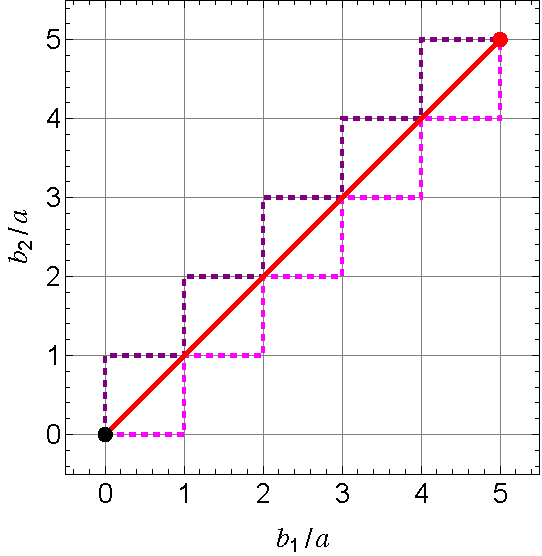
\includegraphics[width=0.3\linewidth]{figures/Example_b_plot_with_2path.pdf}
    \caption{Illustration of path degeneracy for the quark separation vector $\vect{b}$. Distinct step-wise permutations (solid and dashed lines) terminating at the same Cartesian coordinate are averaged to suppress local gauge noise.}
    \label{fig:b_path_example}
\end{figure}
Applying this symmetry-improving operation (path-averaging) strategy across the entire target grid yields the full network of smoothed off-axis trajectories, visualized in Figure \ref{fig:b_full_network}.

\begin{figure}[htpb]
    \centering
    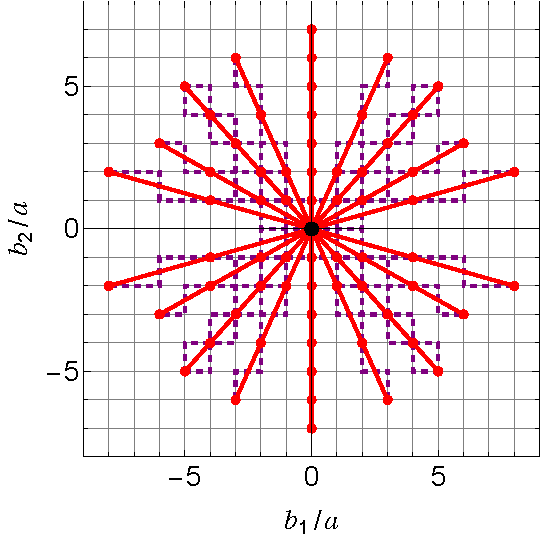
\includegraphics[width=0.4\linewidth]{figures/bL_bT_plot_with_path.pdf}
    \caption{The full network of path-averaged $\vect{b}$ vectors in the $b_1/a - b_2/a$ plane. Solid red lines represent the ideal vectors, while dashed lines illustrate the underlying degenerate staircase paths calculated and averaged on the discrete lattice.}
    \label{fig:b_full_network}
\end{figure}

\begin{widetext}
\section{Solving for the amplitudes}
\label{app:solve}
To extract the physical Sivers shift from the lattice, we must isolate the specific invariant amplitudes $\tAmp_{2B}$ and $\tAmp_{12B}$ from the raw correlator data. We start from the parametrization of the unsubtracted correlator in Eq.~\eqref{eq-phitildedecomp}~\cite{Musch:2011er}. While this parametrization describes a continuous gauge link extending to infinity, we adopt an equivalent representation for lattice calculations in which the structures depend explicitly on the finite staple extent $\eta$. This form remains well defined even in the $v \cdot P = 0$ limit. We obtain it by making the substitution $v \rightarrow \eta v$ and extracting the scaling factors $(v \tcdot P)^{-n}$ as discussed in Appendix~\ref{app:symmetries}:
 \begin{align}
    \frac{1}{2}\widetilde \Phi^{[\gamma^\mu]}_{\unsub}=\frac{1}{2} R_{\gamma^{\mu}} E_N & =  
		P^\mu\, \tilde a_2 - i \mN^2 \bvec^\mu\, \tilde a_3
		- i \mN \epsilon^{\mu \nu \alpha \beta} P_\nu \bvec_\alpha S_\beta\, \tilde a_{12} \nonumber \\ &
		~~+ \mN^2 \eta v^\mu\, \tilde b_1 
		+ \mN \epsilon^{\mu \nu \alpha \beta} P_\nu \eta v_\alpha S_\beta\, \tilde b_7  
		-  i \mN^3 \epsilon^{\mu \nu \alpha \beta} \bvec_\nu \eta v_\alpha S_\beta\, \tilde b_8 \nonumber \\ &
		~~- \mN^3 (\bvec \tcdot S) \epsilon^{\mu \nu \alpha \beta} P_\nu \bvec_\alpha \eta v_\beta\, \tilde b_9
		-i \mN^3 (v \tcdot S) \epsilon^{\mu \nu \alpha \beta} P_\nu \bvec_\alpha \eta^2 v_\beta \tilde b_{10}
\end{align}
To evaluate Eq.~\eqref{eq-phitildedecomp}, we project it onto the kinematics chosen for our lattice setup. We choose a frame where the nucleon moves in the negative $\hat{1}$-direction, the spin is polarized along the $\hat{3}$-axis, and the separation and staple vectors lie in the transverse/longitudinal planes. We set $P^{\mu}=(E_N, -|\vec{P}^1|,0,0)$, $b^{\mu}=(0,b_{1},b_{2},0)$, $v^{\mu}=\pm n^{\prime}(0,v_{1},0,v_{3})$, and $S^{\mu}=(0,0,0,1)$. Throughout this derivation, $\bvec^1$ and $\bvec^2$ denote the contravariant components of $\bvec$, so that $\bvec^1=b_L$ and $\bvec^2=b_T$ in this frame. The invariant dot product is $\bvec\cdot\bvec$; it is the quantity written $\bvec^2$ in the arguments of the amplitudes $\tAmp_i(\bvec^2,\ldots)$ and is never a component. Expanding the sum over Lorentz indices for the temporal component ($\mu = 0$) and canceling the terms that vanish (such as $b^0 = 0$, $v^0 = 0$, and $\bvec \tcdot S = 0$), we find %for each $\gamma^{\mu}$:
\begin{align}
   \frac{1}{2}\widetilde \Phi^{[\gamma^{0}]}_{\unsub}& = P^0\, \tAmp_2  - i \mN  |\vec{P}^1| \bvec_2 S_3\, \tAmp_{12}+ \frac{ i \mN^3}{v \tcdot P}  \bvec_2 v_1 S_3\, \tBmp_8- \frac{i \mN^3}{(v \tcdot P)^2} (v \tcdot S)  |P_1| \bvec_2 v_3 \tBmp_{10}
\end{align}
Repeating this tensor contraction for the longitudinal spatial component ($\mu = 1$), taking care to track the signs of the Levi-Civita symbol, yields:
\begin{align}
   \frac{1}{2}\widetilde \Phi^{[\gamma^{1}]}_{\unsub} & =-|\vec{P}^1|\, \tAmp_2+ \frac{\mN^2}{(v \tcdot P)} v^1\, \tBmp_1 
		+ i \mN  P_0 \bvec_2 S_3\, \tAmp_{12}+ \frac{i \mN^3}{(v \tcdot P)^2} (v \tcdot S)  P_0 \bvec_2 v_3 \tBmp_{10}- i \mN^2 \bvec^1\, \tAmp_3
\end{align}
Evaluating the transverse component ($\mu=2$) isolates terms that depend on $P_0$ and the longitudinal separation $b_1$:
\begin{align}
  \frac{1}{2}\widetilde \Phi^{[\gamma^2]}_{\unsub} & =- i \mN^2 \bvec^2\, \tAmp_3
		- i \mN  P_0 \bvec_1 S_3\, \tAmp_{12}+ \frac{\mN}{v \tcdot P}  P_0 v_1 S_3\, \tBmp_7- \frac{i \mN^3}{(v \tcdot P)^2} (v \tcdot S) P_0 \bvec_1 v_3 \tBmp_{10}
\end{align}
Finally, the orthogonal transverse component ($\mu=3$) simplifies because of the alignment of the spin vector:
\begin{align}
  \frac{1}{2}\widetilde \Phi^{[\gamma^3]}_{\unsub}& = \frac{\mN^2}{(v \tcdot P)} v^3\, \tBmp_1- \frac{i \mN^3}{(v \tcdot P)^2} (v \tcdot S)  P_0 \bvec_2 v_1 \tBmp_{10}
\end{align}
Collecting these results gives the full system of equations mapping the infinite-link continuous amplitudes to the projected correlator components:
\begin{align}
    \frac{1}{2}\widetilde \Phi^{[\gamma^{0}]}_{\unsub}& = P^0\, \tAmp_2  - i \mN  |\vec{P}^1| \bvec_2 S_3\, \tAmp_{12}+ \frac{ i \mN^3}{v \tcdot P}  \bvec_2 v_1 S_3\, \tBmp_8- \frac{i \mN^3}{(v \tcdot P)^2} (v \tcdot S)  |P_1| \bvec_2 v_3 \tBmp_{10}\\
    \frac{1}{2}\widetilde \Phi^{[\gamma^{1}]}_{\unsub} & =-|\vec{P}^1|\, \tAmp_2- i \mN^2 \bvec^1\, \tAmp_3+ \frac{\mN^2}{(v \tcdot P)} v^1\, \tBmp_1 
		+ i \mN  P_0 \bvec_2 S_3\, \tAmp_{12}+ \frac{i \mN^3}{(v \tcdot P)^2} (v \tcdot S)  P_0 \bvec_2 v_3 \tBmp_{10}\\
   \frac{1}{2}\widetilde \Phi^{[\gamma^2]}_{\unsub} & =- i \mN^2 \bvec^2\, \tAmp_3
		- i \mN  P_0 \bvec_1 S_3\, \tAmp_{12}+ \frac{\mN}{v \tcdot P}  P_0 v_1 S_3\, \tBmp_7- \frac{i \mN^3}{(v \tcdot P)^2} (v \tcdot S) P_0 \bvec_1 v_3 \tBmp_{10}\\
    \frac{1}{2}\widetilde \Phi^{[\gamma^3]}_{\unsub}& = \frac{\mN^2}{(v \tcdot P)} v^3\, \tBmp_1- \frac{i \mN^3}{(v \tcdot P)^2} (v \tcdot S)  P_0 \bvec_2 v_1 \tBmp_{10}
\end{align}
We structure this system as a column vector to streamline the upcoming algebraic inversions:
\begin{align}
    \begin{pmatrix}
        \rule{0pt}{16pt} \widetilde \Phi^{[\gamma^{0}]}_{\unsub}\\
        \rule{0pt}{16pt} \widetilde \Phi^{[\gamma^{1}]}_{\unsub}\\
        \rule{0pt}{16pt} \widetilde \Phi^{[\gamma^{2}]}_{\unsub}\\
        \rule{0pt}{16pt} \widetilde \Phi^{[\gamma^{3}]}_{\unsub}
    \end{pmatrix} &=2\begin{pmatrix}
       \rule{0pt}{16pt}  P^0\, \tAmp_2  - i \mN  |\vec{P}^1| \bvec_2 S_3\, \tAmp_{12}+ \frac{ i \mN^3}{v \tcdot P}  \bvec_2 v_1 S_3\, \tBmp_8- \frac{i \mN^3}{(v \tcdot P)^2} (v \tcdot S)  |P_1| \bvec_2 v_3 \tBmp_{10}\\
        \rule{0pt}{16pt} -|\vec{P}^1|\, \tAmp_2- i \mN^2 \bvec^1\, \tAmp_3+ \frac{\mN^2}{(v \tcdot P)} v^1\, \tBmp_1 
		+ i \mN  P_0 \bvec_2 S_3\, \tAmp_{12}+ \frac{i \mN^3}{(v \tcdot P)^2} (v \tcdot S)  P_0 \bvec_2 v_3 \tBmp_{10}\\
         \rule{0pt}{16pt} - i \mN^2 \bvec^2\, \tAmp_3
		- i \mN  P_0 \bvec_1 S_3\, \tAmp_{12}+ \frac{\mN}{v \tcdot P}  P_0 v_1 S_3\, \tBmp_7- \frac{i \mN^3}{(v \tcdot P)^2} (v \tcdot S) P_0 \bvec_1 v_3 \tBmp_{10}\\
        \rule{0pt}{16pt} \frac{\mN^2}{(v \tcdot P)} v^3\, \tBmp_1- \frac{i \mN^3}{(v \tcdot P)^2} (v \tcdot S)  P_0 \bvec_2 v_1 \tBmp_{10}
    \end{pmatrix}
\end{align}
To match standard contravariant Lorentz notation, we raise the spatial indices using the Minkowski metric $g^{\mu\nu} = \text{diag}(1, -1, -1, -1)$. This introduces a relative minus sign for the spatial components (e.g., $P_1 = -P^1$, $b_2 = -b^2$):
\begin{align}
    \begin{pmatrix}
        \rule{0pt}{16pt} \widetilde \Phi^{[\gamma^{0}]}_{\unsub}\\
        \rule{0pt}{16pt} \widetilde \Phi^{[\gamma^{1}]}_{\unsub}\\
        \rule{0pt}{16pt} \widetilde \Phi^{[\gamma^{2}]}_{\unsub}\\
        \rule{0pt}{16pt} \widetilde \Phi^{[\gamma^{3}]}_{\unsub}
    \end{pmatrix} &=2\begin{pmatrix}
       \rule{0pt}{16pt}  P^0\, \tAmp_2  - i \mN  |\vec{P}^1| \bvec^2 S^3\, \tAmp_{12}- \frac{ i \mN^3}{v \tcdot P}  \bvec^2 v^1 S^3\, \tBmp_8- \frac{i \mN^3}{(v \tcdot P)^2} (v \tcdot S)  |\vec{P}^1| \bvec^2 v^3 \tBmp_{10}\\
        \rule{0pt}{16pt} -|\vec{P}^1|\, \tAmp_2- i \mN^2 \bvec^1\, \tAmp_3+ \frac{\mN^2}{(v \tcdot P)} v^1\, \tBmp_1 
		+ i \mN  P^0 \bvec^2 S^3\, \tAmp_{12}+ \frac{i \mN^3}{(v \tcdot P)^2} (v \tcdot S)  P^0 \bvec^2 v^3 \tBmp_{10}\\
         \rule{0pt}{16pt} - i \mN^2 \bvec^2\, \tAmp_3
		- i \mN  P^0 \bvec^1 S^3\, \tAmp_{12}+ \frac{\mN}{v \tcdot P}  P^0 v^1 S^3\, \tBmp_7- \frac{i \mN^3}{(v \tcdot P)^2} (v \tcdot S) P^0 \bvec^1 v^3 \tBmp_{10}\\
        \rule{0pt}{16pt} \frac{\mN^2}{(v \tcdot P)} v^3\, \tBmp_1- \frac{i \mN^3}{(v \tcdot P)^2} (v \tcdot S)  P^0 \bvec^2 v^1 \tBmp_{10}
    \end{pmatrix}
\end{align}
To connect these continuous amplitudes to the discretized finite-link observables simulated on the lattice, we use the mapping of Eq.~\eqref{eq-ab} between the infinite-link amplitudes ($\tAmp_i$, $\tBmp_i$) and the finite-link amplitudes ($\tilde{a}_i$, $\tilde{b}_i$). The finite-link amplitudes are complex-valued functions, which we decompose into their real and imaginary components:
\begin{align}
    \tilde{a}_i&=\tilde{a}^{\text{Re}}_i+i\tilde{a}^{\text{Im}}_i\\
    \tilde{b}_i&=\tilde{b}^{\text{Re}}_i+i\tilde{b}^{\text{Im}}_i
\end{align}
The lattice evaluation also requires converting the continuous Minkowski gamma matrices ($\gamma_M$) into the Euclidean conventions ($\gamma_E$) used by the lattice simulation software:
\begin{itemize}
    \item Correct Euclidean $\longleftrightarrow$ Minkowski $\gamma$-matrices notation:
    \begin{align}
        \gamma^{1}_{E}=&+i\gamma^{1}_{M}\\
        \gamma^{2}_{E}=&-i\gamma^{2}_{M}\\
        \gamma^{3}_{E}=&+i\gamma^{3}_{M}\\
        \gamma^{4}_{E}=&\gamma^{0}_{M}\\
        \gamma^{5}_{E}=&\gamma^{1}_{E}\gamma^{2}_{E}\gamma^{3}_{E}\gamma^{4}_{E}=-\gamma^{5}_{M}=-i\gamma^{0}_{M}\gamma^{1}_{M}\gamma^{2}_{M}\gamma^{3}_{M}
    \end{align}
\end{itemize}
Substituting the Euclidean gamma structures and mapping $P^0 \to E_N$, we rewrite the column vector entirely in terms of the lattice ratio observables $R_{\Gamma(i)}$ and the finite-link amplitudes. The index $i \in \{1,2,4,8\}$ labels each Dirac structure by its bit-encoded position (CHROMA and QLUA convention) in our operator basis, matching the correspondence $\Gamma(1)=[+i\gamma^1]$, $\Gamma(2)=[-i\gamma^2]$, $\Gamma(4)=[+i\gamma^3]$, and $\Gamma(8)=[\gamma^0]$ used below:
\begin{align}
    \begin{pmatrix}
        \rule{0pt}{16pt} R_{\Gamma(1)}\\
        \rule{0pt}{16pt} R_{\Gamma(2)}\\
        \rule{0pt}{16pt} R_{\Gamma(4)}\\
        \rule{0pt}{16pt} R_{\Gamma(8)}
    \end{pmatrix} = \begin{pmatrix}
        \rule{0pt}{16pt} R_{[+i\gamma^1]}\\
        \rule{0pt}{16pt} R_{[-i\gamma^2]}\\
        \rule{0pt}{16pt} R_{[+i\gamma^3]}\\
        \rule{0pt}{16pt} R_{[\gamma^0]}
    \end{pmatrix} &=2\begin{pmatrix}
        \rule{0pt}{16pt} -i\frac{|\vec{P}^1|}{E_N}\, \tilde a_2+  \frac{\mN^2}{E_N} \bvec^1\, \tilde a_3+ i\frac{\mN^2}{E_N} \eta v^1\, \tilde b_1 
		-  \mN  \bvec^2 \, \tilde a_{12}+  \mN^3  \bvec^2 \eta^2 (v^3)^2 \tilde b_{10}\\
         \rule{0pt}{16pt} -  \frac{\mN^2}{E_N} \bvec^2\, \tilde a_3
		-  \mN   \bvec^1  \tilde a_{12}-i \mN \eta  v^1  \tilde b_7+ \mN^3  \bvec^1 \eta^2 (v^3)^2 \tilde b_{10}\\
        \rule{0pt}{16pt} i\frac{\mN^2}{E_N} \eta v^3\, \tilde b_1-  \mN^3 \bvec^2 \eta^2 v^1 v^3\tilde b_{10}\\
         \rule{0pt}{16pt}   \tilde a_2  - i \mN  \frac{|\vec{P}^1|}{E_N} \bvec^2  \tilde a_{12}- \frac{ i \mN^3}{E_N}  \bvec^2 \eta v^1  \tilde b_8+ \frac{i \mN^3}{E_N}  |\vec{P}^1| \bvec^2 \eta^2 (v^3)^2 \tilde b_{10}
    \end{pmatrix}
\end{align}
To separate the real and imaginary amplitude contributions analytically, we split this matrix equation into two sets by flipping the longitudinal separation component $b^1$. For a strictly positive longitudinal separation ($+b^1$), writing out the real and imaginary parts of the correlator ratios gives:
\begin{align}
    \begin{pmatrix}
        \rule{0pt}{16pt} \text{Re}\{ R_{\Gamma(1)}\}^{[+b^1]} \\
        \rule{0pt}{16pt} \text{Im}\{ R_{\Gamma(1)}\}^{[+b^1]} \\
        \rule{0pt}{16pt} \text{Re}\{ R_{\Gamma(2)}\}^{[+b^1]} \\
        \rule{0pt}{16pt} \text{Im}\{ R_{\Gamma(2)}\}^{[+b^1]} \\
        \rule{0pt}{16pt} \text{Re}\{ R_{\Gamma(4)}\}^{[+b^1]} \\
        \rule{0pt}{16pt} \text{Im}\{ R_{\Gamma(4)}\}^{[+b^1]} \\
        \rule{0pt}{16pt} \text{Re}\{ R_{\Gamma(8)}\}^{[+b^1]} \\
        \rule{0pt}{16pt} \text{Im}\{ R_{\Gamma(8)}\}^{[+b^1]}
    \end{pmatrix} &= 2\begin{pmatrix}
     \rule{0pt}{16pt}   \frac{\mN^2}{E_N} \bvec^1\, \tilde a^{\text{Re}}_3-  \mN  \bvec^2 \, \tilde a^{\text{Re}}_{12}+  \mN^3  \bvec^2 \eta^2 (v^3)^2 \tilde b^{\text{Re}}_{10} +\frac{|\vec{P}^1|}{E_N}\, \tilde a^{\text{Im}}_2- \frac{\mN^2}{E_N} \eta v^1\, \tilde b^{\text{Im}}_1\\
      \rule{0pt}{16pt}  -\frac{|\vec{P}^1|}{E_N}\, \tilde a^{\text{Re}}_2+ \frac{\mN^2}{E_N} \eta v^1\, \tilde b^{\text{Re}}_1 + \frac{\mN^2}{E_N} \bvec^1\, \tilde a^{\text{Im}}_3-  \mN  \bvec^2 \, \tilde a^{\text{Im}}_{12}+  \mN^3  \bvec^2 \eta^2 (v^3)^2 \tilde b^{\text{Im}}_{10}\\
      \rule{0pt}{16pt}  -  \frac{\mN^2}{E_N} \bvec^2\, \tilde a^{\text{Re}}_3
		-  \mN   \bvec^1  \tilde a^{\text{Re}}_{12}+ \mN^3  \bvec^1 \eta^2 (v^3)^2 \tilde b^{\text{Re}}_{10}+\mN \eta v^1  \tilde b^{\text{Im}}_7 \\
      \rule{0pt}{16pt} - \mN \eta v^1  \tilde b^{\text{Re}}_7 -  \frac{\mN^2}{E_N} \bvec^2\, \tilde a^{\text{Im}}_3
		-  \mN   \bvec^1  \tilde a^{\text{Im}}_{12}+ \mN^3  \bvec^1 \eta^2 (v^3)^2 \tilde b^{\text{Im}}_{10}\\
      \rule{0pt}{16pt} -\mN^3 \bvec^2 \eta^2 v^1 v^3\tilde b^{\text{Re}}_{10}-\frac{\mN^2}{E_N} \eta v^3\, \tilde b^{\text{Im}}_1\\
      \rule{0pt}{16pt} \frac{\mN^2}{E_N} \eta v^3\, \tilde b^{\text{Re}}_1 -\mN^3 \bvec^2 \eta^2 v^1 v^3\tilde b^{\text{Im}}_{10}\\
      \rule{0pt}{16pt}  \tilde a^{\text{Re}}_2 +  \mN  \frac{|\vec{P}^1|}{E_N} \bvec^2  \tilde a^{\text{Im}}_{12}+ \frac{  \mN^3}{E_N}  \bvec^2 \eta v^1  \tilde b^{\text{Im}}_8- \frac{ \mN^3}{E_N}  |\vec{P}^1| \bvec^2 \eta^2 (v^3)^2 \tilde b^{\text{Im}}_{10}\\
      \rule{0pt}{16pt} -  \mN  \frac{|\vec{P}^1|}{E_N} \bvec^2  \tilde a^{\text{Re}}_{12}- \frac{  \mN^3}{E_N}  \bvec^2 \eta v^1  \tilde b^{\text{Re}}_8+ \frac{ \mN^3}{E_N}  |\vec{P}^1| \bvec^2 \eta^2 (v^3)^2 \tilde b^{\text{Re}}_{10}+\tilde a^{\text{Im}}_2
    \end{pmatrix}
\end{align}
Evaluating the system for the negated separation ($-b^1$) flips the signs of selected terms according to the parity constraints of Eq.~\eqref{eq-ReIm-parity}. By construction, the imaginary parts of the amplitudes are odd functions of $b^1$ ($\tAmp_i^{\text{Im}}=\tAmp_i^{\text{(b-odd)}}=\tAmp_i^{\text{($b^1$-odd)}}$ and  $\tBmp_i^{\text{Im}}=\tBmp_i^{\text{(b-odd)}}=\tBmp_i^{\text{($b^1$-odd)}}$). Applying these parity reversals yields the conjugate matrix:
\begin{align}
    \begin{pmatrix}
        \rule{0pt}{16pt} \text{Re}\{ R_{\Gamma(1)}\}^{[-b^1]} \\
        \rule{0pt}{16pt} \text{Im}\{ R_{\Gamma(1)}\}^{[-b^1]} \\
        \rule{0pt}{16pt} \text{Re}\{ R_{\Gamma(2)}\}^{[-b^1]} \\
        \rule{0pt}{16pt} \text{Im}\{ R_{\Gamma(2)}\}^{[-b^1]} \\
        \rule{0pt}{16pt} \text{Re}\{ R_{\Gamma(4)}\}^{[-b^1]} \\
        \rule{0pt}{16pt} \text{Im}\{ R_{\Gamma(4)}\}^{[-b^1]} \\
        \rule{0pt}{16pt} \text{Re}\{ R_{\Gamma(8)}\}^{[-b^1]} \\
        \rule{0pt}{16pt} \text{Im}\{ R_{\Gamma(8)}\}^{[-b^1]}
    \end{pmatrix} &= 2\begin{pmatrix}
     \rule{0pt}{16pt}   \textcolor{red}{-}\frac{\mN^2}{E_N} \bvec^1\, \tilde a^{\text{Re}}_3-  \mN  \bvec^2 \, \tilde a^{\text{Re}}_{12}+  \mN^3  \bvec^2 \eta^2 (v^3)^2 \tilde b^{\text{Re}}_{10} \textcolor{red}{-}\frac{|\vec{P}^1|}{E_N}\, \tilde a^{\text{Im}}_2\textcolor{red}{+} \frac{\mN^2}{E_N} \eta v^1\, \tilde b^{\text{Im}}_1\\
      \rule{0pt}{16pt}  -\frac{|\vec{P}^1|}{E_N}\, \tilde a^{\text{Re}}_2+ \frac{\mN^2}{E_N} \eta v^1\, \tilde b^{\text{Re}}_1 + \frac{\mN^2}{E_N} \bvec^1\, \tilde a^{\text{Im}}_3\textcolor{red}{+} \mN  \bvec^2 \, \tilde a^{\text{Im}}_{12}\textcolor{red}{-} \mN^3  \bvec^2 \eta^2 (v^3)^2 \tilde b^{\text{Im}}_{10}\\
      \rule{0pt}{16pt}  - \frac{\mN^2}{E_N} \bvec^2\, \tilde a^{\text{Re}}_3
		\textcolor{red}{+}  \mN   \bvec^1  \tilde a^{\text{Re}}_{12}\textcolor{red}{-} \mN^3  \bvec^1 \eta^2 (v^3)^2 \tilde b^{\text{Re}}_{10}\textcolor{red}{-}\mN \eta v^1  \tilde b^{\text{Im}}_7 \\
      \rule{0pt}{16pt} - \mN \eta v^1  \tilde b^{\text{Re}}_7 \textcolor{red}{+}  \frac{\mN^2}{E_N} \bvec^2\, \tilde a^{\text{Im}}_3
		- \mN   \bvec^1  \tilde a^{\text{Im}}_{12} +\mN^3  \bvec^1 \eta^2 (v^3)^2 \tilde b^{\text{Im}}_{10}\\
      \rule{0pt}{16pt}-\mN^3 \bvec^2 \eta^2 v^1 v^3\tilde b^{\text{Re}}_{10}\textcolor{red}{+}\frac{\mN^2}{E_N} \eta v^3\, \tilde b^{\text{Im}}_1\\
      \rule{0pt}{16pt} \frac{\mN^2}{E_N} \eta v^3\, \tilde b^{\text{Re}}_1 \textcolor{red}{+} \mN^3 \bvec^2 \eta^2 v^1 v^3\tilde b^{\text{Im}}_{10}\\
      \rule{0pt}{16pt}  \tilde a^{\text{Re}}_2 \textcolor{red}{-}  \mN  \frac{|\vec{P}^1|}{E_N} \bvec^2  \tilde a^{\text{Im}}_{12}\textcolor{red}{-} \frac{  \mN^3}{E_N}  \bvec^2 \eta v^1  \tilde b^{\text{Im}}_8\textcolor{red}{+} \frac{ \mN^3}{E_N}  |\vec{P}^1| \bvec^2 \eta^2 (v^3)^2 \tilde b^{\text{Im}}_{10}\\
      \rule{0pt}{16pt} - \mN  \frac{|\vec{P}^1|}{E_N} \bvec^2  \tilde a^{\text{Re}}_{12}- \frac{  \mN^3}{E_N}  \bvec^2 \eta v^1  \tilde b^{\text{Re}}_8 + \frac{ \mN^3}{E_N}  |\vec{P}^1| \bvec^2 \eta^2 (v^3)^2 \tilde b^{\text{Re}}_{10}\textcolor{red}{-}\tilde a^{\text{Im}}_2
    \end{pmatrix}
\end{align}
By taking the symmetric average of the two matrices, $\frac{1}{2}\left(R^{[+b]} + R^{[-b]}\right)$, we project out the $b$-even combination, isolating the real parts of the requisite amplitudes:
\begin{align}
    \begin{pmatrix}
        \rule{0pt}{16pt} \text{Re}\{ R_{\Gamma(1)}\}^{[b^{1}\text{-even}]} \\
        \rule{0pt}{16pt} \text{Im}\{ R_{\Gamma(1)}\}^{[b^{1}\text{-even}]} \\
        \rule{0pt}{16pt} \text{Re}\{ R_{\Gamma(2)}\}^{[b^{1}\text{-even}]} \\
        \rule{0pt}{16pt} \text{Im}\{ R_{\Gamma(2)}\}^{[b^{1}\text{-even}]} \\
        \rule{0pt}{16pt} \text{Re}\{ R_{\Gamma(4)}\}^{[b^{1}\text{-even}]} \\
        \rule{0pt}{16pt} \text{Im}\{ R_{\Gamma(4)}\}^{[b^{1}\text{-even}]} \\
        \rule{0pt}{16pt} \text{Re}\{ R_{\Gamma(8)}\}^{[b^{1}\text{-even}]} \\
        \rule{0pt}{16pt} \text{Im}\{ R_{\Gamma(8)}\}^{[b^{1}\text{-even}]}
    \end{pmatrix} &= 2\begin{pmatrix}
     \rule{0pt}{16pt}  -  \mN  \bvec^2 \, \tilde a^{\text{Re}}_{12}+  \mN^3  \bvec^2 \eta^2 (v^3)^2 \tilde b^{\text{Re}}_{10} \\
      \rule{0pt}{16pt}  -\frac{|\vec{P}^1|}{E_N}\, \tilde a^{\text{Re}}_2+ \frac{\mN^2}{E_N} \eta v^1\, \tilde b^{\text{Re}}_1 + \frac{\mN^2}{E_N} \bvec^1\, \tilde a^{\text{Im}}_3\\
      \rule{0pt}{16pt}  -  \frac{\mN^2}{E_N} \bvec^2\, \tilde a^{\text{Re}}_3
		\\
      \rule{0pt}{16pt} - \mN \eta v^1  \tilde b^{\text{Re}}_7
		-  \mN   \bvec^1  \tilde a^{\text{Im}}_{12}+ \mN^3  \bvec^1 \eta^2 (v^3)^2 \tilde b^{\text{Im}}_{10}\\
      \rule{0pt}{16pt} -\mN^3 \bvec^2 \eta^2 v^1 v^3\tilde b^{\text{Re}}_{10}\\
      \rule{0pt}{16pt} \frac{\mN^2}{E_N} \eta v^3\, \tilde b^{\text{Re}}_1 \\
      \rule{0pt}{16pt}  \tilde a^{\text{Re}}_2\\
      \rule{0pt}{16pt} -  \mN  \frac{|\vec{P}^1|}{E_N} \bvec^2  \tilde a^{\text{Re}}_{12}- \frac{  \mN^3}{E_N}  \bvec^2 \eta v^1  \tilde b^{\text{Re}}_8+ \frac{ \mN^3}{E_N}  |\vec{P}^1| \bvec^2 \eta^2 (v^3)^2 \tilde b^{\text{Re}}_{10}
    \end{pmatrix}
\end{align}
Conversely, taking the antisymmetric half-difference of the two matrices, $\frac{1}{2}\left(R^{[+b]} - R^{[-b]}\right)$, projects out the $b$-odd combination, isolating the imaginary parts:
\begin{align}
    \begin{pmatrix}
        \rule{0pt}{16pt} \text{Re}\{ R_{\Gamma(1)}\}^{[b^{1}\text{-odd}]} \\
        \rule{0pt}{16pt} \text{Im}\{ R_{\Gamma(1)}\}^{[b^{1}\text{-odd}]} \\
        \rule{0pt}{16pt} \text{Re}\{ R_{\Gamma(2)}\}^{[b^{1}\text{-odd}]} \\
        \rule{0pt}{16pt} \text{Im}\{ R_{\Gamma(2)}\}^{[b^{1}\text{-odd}]} \\
        \rule{0pt}{16pt} \text{Re}\{ R_{\Gamma(4)}\}^{[b^{1}\text{-odd}]} \\
        \rule{0pt}{16pt} \text{Im}\{ R_{\Gamma(4)}\}^{[b^{1}\text{-odd}]} \\
        \rule{0pt}{16pt} \text{Re}\{ R_{\Gamma(8)}\}^{[b^{1}\text{-odd}]} \\
        \rule{0pt}{16pt} \text{Im}\{ R_{\Gamma(8)}\}^{[b^{1}\text{-odd}]}
    \end{pmatrix} &= 2\begin{pmatrix}
     \rule{0pt}{16pt}   \frac{\mN^2}{E_N} \bvec^1\, \tilde a^{\text{Re}}_3+\frac{|\vec{P}^1|}{E_N}\, \tilde a^{\text{Im}}_2- \frac{\mN^2}{E_N} \eta v^1\, \tilde b^{\text{Im}}_1\\
      \rule{0pt}{16pt}  -  \mN  \bvec^2 \, \tilde a^{\text{Im}}_{12}+  \mN^3  \bvec^2 \eta^2 (v^3)^2 \tilde b^{\text{Im}}_{10}\\
      \rule{0pt}{16pt}  
		-  \mN   \bvec^1  \tilde a^{\text{Re}}_{12}+ \mN^3  \bvec^1 \eta^2 (v^3)^2 \tilde b^{\text{Re}}_{10}+\mN \eta v^1  \tilde b^{\text{Im}}_7 \\
      \rule{0pt}{16pt}  -  \frac{\mN^2}{E_N} \bvec^2\, \tilde a^{\text{Im}}_3\\
      \rule{0pt}{16pt} -\frac{\mN^2}{E_N} \eta v^3\, \tilde b^{\text{Im}}_1\\
      \rule{0pt}{16pt}  -\mN^3 \bvec^2 \eta^2 v^1 v^3\tilde b^{\text{Im}}_{10}\\
      \rule{0pt}{16pt}    \mN  \frac{|\vec{P}^1|}{E_N} \bvec^2  \tilde a^{\text{Im}}_{12}+ \frac{  \mN^3}{E_N}  \bvec^2 \eta v^1  \tilde b^{\text{Im}}_8- \frac{ \mN^3}{E_N}  |\vec{P}^1| \bvec^2 \eta^2 (v^3)^2 \tilde b^{\text{Im}}_{10}\\
      \rule{0pt}{16pt} \tilde a^{\text{Im}}_2
    \end{pmatrix}
\end{align}
To analytically reconstruct the Sivers shift, we solve these projected systems for the amplitudes that drive the Sivers effect: $\tilde a_2$, $\tilde b_1$, $\tilde a_{12}$, and $\tilde b_8$. Reading directly from the $b$-even system, we isolate the real components:
\begin{align}
    \tilde a^{\text{Re}}_2 = & \frac{1}{2}\text{Re}\{ R_{\Gamma(8)}\}^{[b^{1}\text{-even}]} \\
    \tilde b^{\text{Re}}_1 = & \frac{E_{N}}{2\mN^2 \eta v^3} \text{Im}\{ R_{\Gamma(4)}\}^{[b^{1}\text{-even}]}
\end{align}
Substituting the appropriate matrix rows, we decouple $\tilde a_{12}$ and $\tilde b_8$:
\begin{align}
   \tilde a^{\text{Re}}_{12}=&\frac{-1}{2\mN  \bvec^2}\left[\text{Re}\{ R_{\Gamma(1)}\}^{[b^{1}\text{-even}]}+\frac{v^3}{v^1}\text{Re}\{ R_{\Gamma(4)}\}^{[b^{1}\text{-even}]}\right]
\end{align}
\begin{align}
    \tilde b^{\text{Re}}_8=&\frac{-E_N}{ 2\mN^3 \bvec^2 \eta v^1 }\left[\text{Im}\{ R_{\Gamma(8)}\}^{[b^{1}\text{-even}]}+\frac{|\vec{P}^1|v^3}{E_N v^1}\text{Re}\{ R_{\Gamma(4)}\}^{[b^{1}\text{-even}]}+ 2\mN  \frac{|\vec{P}^1|}{E_N} \bvec^2  \tilde a^{\text{Re}}_{12}\right]
\end{align}
Applying identical algebraic decoupling to the $b$-odd system, we isolate the corresponding imaginary components:
\begin{align}
    \tilde a^{\text{Im}}_2 = & \frac{1}{2}\text{Im}\{ R_{\Gamma(8)}\}^{[b^{1}\text{-odd}]} \\
    \tilde b^{\text{Im}}_1 = & \frac{-E_{N}}{2\mN^2 \eta v^3} \text{Re}\{ R_{\Gamma(4)}\}^{[b^{1}\text{-odd}]}
\end{align}
and the remaining transverse amplitudes:
\begin{align}
   \tilde a^{\text{Im}}_{12}=&\frac{-1}{2\mN  \bvec^2}\left[\text{Im}\{ R_{\Gamma(1)}\}^{[b^{1}\text{-odd}]}+\frac{v^3}{v^1}\text{Im}\{ R_{\Gamma(4)}\}^{[b^{1}\text{-odd}]}\right]
\end{align}
\begin{align}
    \tilde b^{\text{Im}}_8=&\frac{E_N}{ 2\mN^3 \bvec^2 \eta v^1 }\left[\text{Re}\{ R_{\Gamma(8)}\}^{[b^{1}\text{-odd}]}-\frac{|\vec{P}^1|v^3}{E_N v^1}\text{Im}\{ R_{\Gamma(4)}\}^{[b^{1}\text{-odd}]}- 2\mN  \frac{|\vec{P}^1|}{E_N} \bvec^2  \tilde a^{\text{Im}}_{12}\right]
\end{align}
Finally, we convert these finite-link evaluations ($\tilde a_i, \tilde b_i$) back into the standard continuum-invariant amplitudes ($\tAmp_i, \tBmp_i$) using the proportionality dictionary:
\begin{align}
	\tAmp_i & = \tilde a_i \\
	 \tBmp_i & = (\eta v \tcdot P)^n\ \tilde b_i
\end{align}
\end{widetext}

\section{Fit exploration}
\label{app:fit_exploration}
The fits below support the choice of the coupled Lorentzian power law (Sec.~\ref{sec:power_law}) and of the $\eta$ dependence (Sec.~\ref{sec:eta_dependence}). All fits are for $P_L=-2$, $|\vect b|\ge3a$ and $6\le\eta\le10$.


\subsection{Exponential decay in $|\vect b|$}

Fig.~\ref{fig:exp_straight} is the straight-line test for an exponential decay $\tAmp_{2B}^{\text{Re}}\propto e^{-c|\vect b|}$ in $|\vect b|=\sqrt{b^2}$. We fit $Ae^{-c|\vect b|}e^{-f\eta}$ with the loss of Eq.~\eqref{eq:pysr_loss}, which gives $c=0.685$ and $\mathcal L=1.42$ for three parameters, and $\mathcal L=1.31$ when a constant offset is added. For comparison, the \texttt{PySR} models of Table~\ref{tab:pysr_pareto} have $\mathcal L=1.61$ at $C=13$, $1.38$ at $C=15$ (five parameters) and $1.26$ at $C=17$. Over $3\le|\vect b|/a\le8.2$ the exponential in $|\vect b|$ therefore describes the data about as well as the power-law models, with fewer parameters. The search library has no function of $|\vect b|$ alone, so the Pareto front does not test this form. The separable ansätze of Sec.~\ref{sec:power_law} apply it to all three amplitudes.

\begin{figure*}[!p]
\centering
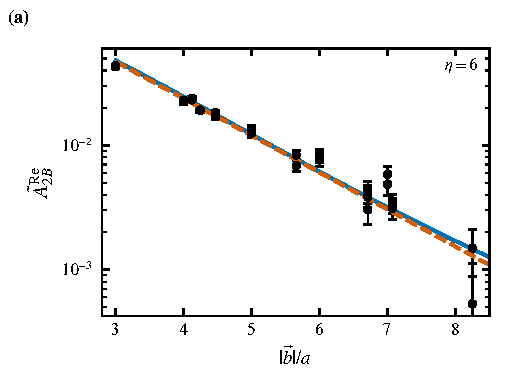
\includegraphics[width=\panelw]{figures/panels/pysr/exp_eta6.pdf}\hfill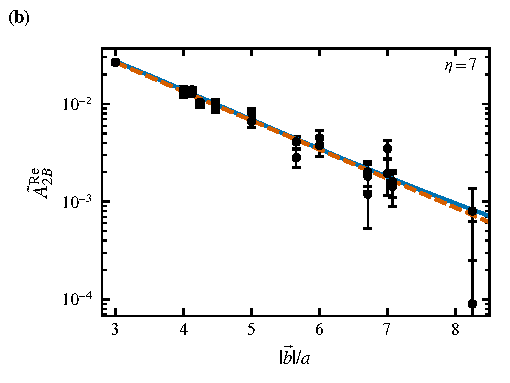
\includegraphics[width=\panelw]{figures/panels/pysr/exp_eta7.pdf}\par
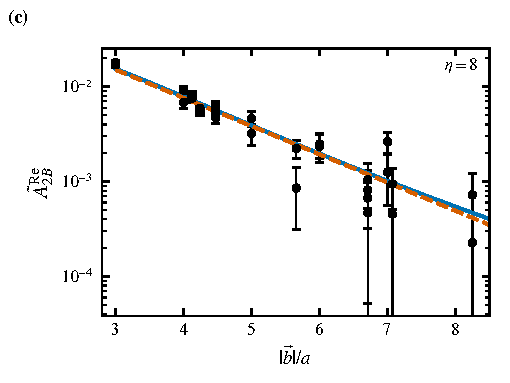
\includegraphics[width=\panelw]{figures/panels/pysr/exp_eta8.pdf}\hfill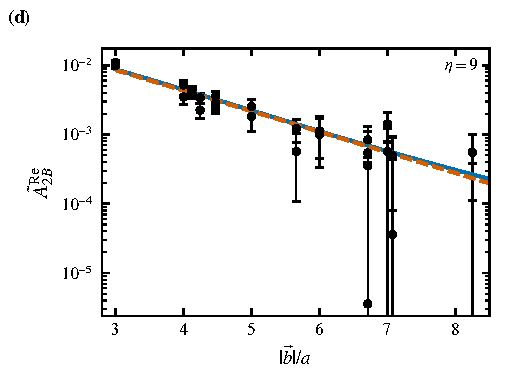
\includegraphics[width=\panelw]{figures/panels/pysr/exp_eta9.pdf}\par
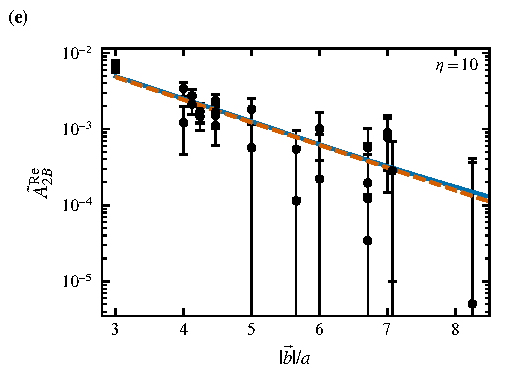
\includegraphics[width=\panelw]{figures/panels/pysr/exp_eta10.pdf}\hfill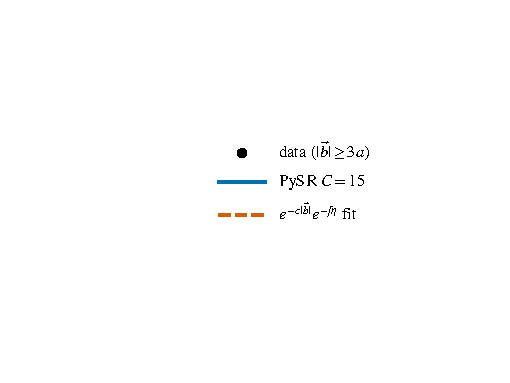
\includegraphics[width=\panelw]{figures/panels/pysr/exp_legend.pdf}
\caption{Panels (a)--(e): $\eta=6,7,8,9,10$. Straight-line test for an exponential decay in $|\vect b|=\sqrt{b^2}$ at $P_L=-2$. A profile $\tAmp_{2B}^{\text{Re}}\propto e^{-c|\vect b|}$ is a straight line on a logarithmic ordinate. The best fit (red dashed, $c=0.685$, $\mathcal L=1.42$) and the $C=15$ \texttt{PySR} model (blue, $\mathcal L=1.38$) both follow the data over $3\le|\vect b|/a\le8.2$.}
\label{fig:exp_straight}
\end{figure*}

\subsection{Gaussian and power-law fits with $\eta$-dependent widths}

Tables~\ref{tab:gauss_family_PL2} and~\ref{tab:powerlaw_family_PL2} list, for each model, the fit parameters and the correlated $\chi^2/\text{dof}$. The Gaussian ansätze reach $\chi^2/\text{dof}=1.56$ at best, against $1.10$ to $1.24$ for the power-law forms. The power-law forms with an $\eta$-dependent $c$ ($c(1-k_1/\eta)$, $c(1-k_1/\eta-k_2/\eta^2)$ and the wider forms) all give $\chi^2/\text{dof}\approx1.12$, so the data do not single out one $c(\eta)$, and the choice rests on the criteria of Sec.~\ref{sec:simultaneous_fit}.

Tables~\ref{tab:sep_EE_PL2}--\ref{tab:sep_EP_PL2} list separable ansätze, a longitudinal factor in $|b_LP_L|$ times a transverse factor in $b$, with the same $\eta$ dependences $c(\eta)$ of the longitudinal coefficient and a constant $d$: an exponential longitudinal and an exponential transverse factor, a power-law longitudinal and an exponential transverse factor, and an exponential longitudinal and a power-law transverse factor.

\begin{table*}
\caption{Fits of $\tAmp_{2B}^{\text{Re}}(b_L,b_T,\eta)$ at $P_L=-2$ ($|\vect b|\ge3a$, $6\le\eta\le10$) to $a\,e^{-f\eta}\exp[-c(\eta)(b_LP_L)^2-d(\eta)(b_L^2+b_T^2)]$. Each row $(i,j)$ uses $c(\eta)=c\,g_i(\eta)$ and $d(\eta)=d\,h_j(\eta)$ with $g_0=h_0=1$, $g_1=1-k_{c1}/\eta$, $g_2=1+k_{c1}/\eta-k_{c2}/\sqrt{\eta}$, $g_3=1-k_{c1}/\eta-k_{c2}/\eta^2$, and $h_1$, $h_2$, $h_3$ the same forms with $k_{d1}$, $k_{d2}$. Here $c$ multiplies $(b_LP_L)^2$, so it differs from the $c$ of the other tables by $P_L^2$. The $\chi^2/\mathrm{dof}$ is the correlated value with the full jackknife covariance matrix of the $\tAmp_{2B}^{\text{Re}}$ rows, from \texttt{lsqfit} (singular-value cut $10^{-12}$), given as the jackknife mean (error) over the 2903 jackknife columns (including the central value), as in the simultaneous fits, but without cross-amplitude correlations. The fits are unconstrained, and the number of degrees of freedom is the number of rows minus the number of parameters, counting all rows including the duplicated ($b_L\to-b_L$) rows. Rows marked with $^\dagger$ have shape parameters ($k_{\ldots}$, $\nu$) that are unconstrained (error $\ge$ value) or degenerate (value $>10^4$); only combinations of the parameters, not their individual values, are determined by the data.}
\label{tab:gauss_family_PL2}
\scriptsize
\begin{ruledtabular}
\begin{tabular}{l@{\hspace{3pt}}c@{\hspace{3pt}}c@{\hspace{3pt}}c@{\hspace{3pt}}c@{\hspace{3pt}}c@{\hspace{3pt}}c@{\hspace{3pt}}c@{\hspace{3pt}}c@{\hspace{3pt}}c}
$(i,j)$ & $a$ & $c$ & $k_{c1}$ & $k_{c2}$ & $d$ & $k_{d1}$ & $k_{d2}$ & $f$ & $\chi^2/\mathrm{dof}$ \\
\hline
$(0,0)$ & $2.09(14)$ & $-0.00169(68)$ &  &  & $0.0860(32)$ &  &  & $0.530(11)$ & $1.91(19)$ \\
$(0,1)$ & $0.918(94)$ & $-0.00116(66)$ &  &  & $0.173(11)$ & $2.88(17)$ &  & $0.382(18)$ & $1.57(17)$ \\
$(0,2)$ & $0.821(97)$ & $-0.00111(66)$ &  &  & $0.39(11)$ & $2.0(11)$ & $2.72(62)$ & $0.362(21)$ & $1.56(17)$ \\
$(0,3)$ & $0.837(98)$ & $-0.00111(66)$ &  &  & $0.231(37)$ & $5.2(10)$ & $-9.1(41)$ & $0.365(20)$ & $1.57(17)$ \\
$(1,0)$ & $1.52(12)$ & $0.0170(33)$ & $5.99(26)$ &  & $0.0840(31)$ &  &  & $0.474(13)$ & $1.74(18)$ \\
$(1,1)$$^\dagger$ & $0.934(97)$ & $0.0015(42)$ & $10(13)$ &  & $0.166(15)$ & $2.77(24)$ &  & $0.385(18)$ & $1.58(17)$ \\
$(1,2)$$^\dagger$ & $0.83(10)$ & $-0.0004(45)$ & $-10(336)$ &  & $0.39(12)$ & $2.0(12)$ & $2.71(64)$ & $0.363(22)$ & $1.57(17)$ \\
$(1,3)$$^\dagger$ & $0.85(10)$ & $-0.0001(32)$ & $0.0(15)\times10^{5}$ &  & $0.226(40)$ & $5.1(11)$ & $-9.0(43)$ & $0.367(21)$ & $1.58(17)$ \\
$(2,0)$$^\dagger$ & $1.51(12)$ & $0.044(42)$ & $1.6(45)$ & $3.1(18)$ & $0.0839(31)$ &  &  & $0.473(13)$ & $1.75(18)$ \\
$(2,1)$ & $0.875(94)$ & $0.088(40)$ & $6.31(58)$ & $5.05(25)$ & $0.173(16)$ & $2.90(23)$ &  & $0.373(19)$ & $1.57(17)$ \\
$(2,2)$$^\dagger$ & $0.86(11)$ & $0.072(60)$ & $6.33(71)$ & $5.07(31)$ & $0.23(18)$ & $-0.7(50)$ & $1.2(27)$ & $0.369(23)$ & $1.57(17)$ \\
$(2,3)$$^\dagger$ & $0.88(11)$ & $0.093(59)$ & $6.30(55)$ & $5.05(24)$ & $0.167(56)$ & $2.6(30)$ & $1(12)$ & $0.375(22)$ & $1.57(17)$ \\
$(3,0)$$^\dagger$ & $1.51(12)$ & $0.023(13)$ & $7.7(26)$ & $-11(16)$ & $0.0839(31)$ &  &  & $0.473(13)$ & $1.75(18)$ \\
$(3,1)$ & $0.881(94)$ & $0.023(12)$ & $13.0(14)$ & $-40.4(75)$ & $0.172(16)$ & $2.88(23)$ &  & $0.375(19)$ & $1.57(17)$ \\
$(3,2)$$^\dagger$ & $0.85(11)$ & $0.016(19)$ & $13.3(24)$ & $-41(12)$ & $0.27(18)$ & $0.3(37)$ & $1.7(21)$ & $0.368(23)$ & $1.58(17)$ \\
$(3,3)$$^\dagger$ & $0.88(11)$ & $0.022(18)$ & $13.0(15)$ & $-40.5(79)$ & $0.177(57)$ & $3.1(28)$ & $-1(11)$ & $0.374(22)$ & $1.58(17)$ \\
\end{tabular}
\end{ruledtabular}
\end{table*}

\begin{table*}
\caption{Fits of $\tAmp_{2B}^{\text{Re}}$ at $P_L=-2$ ($|\vect b|\ge3a$, $6\le\eta\le10$) to $a\,e^{-f\eta}\big/\{1+[d+c\,g(\eta)]b_L^2+d\,b_T^2\}^{j}$ for different $c(\eta)=c\,g(\eta)$. The $\chi^2/\mathrm{dof}$ is the correlated value, given as the jackknife mean (error).}
\label{tab:powerlaw_family_PL2}
\scriptsize
\begin{ruledtabular}
\begin{tabular}{l@{\hspace{3pt}}c@{\hspace{3pt}}c@{\hspace{3pt}}c@{\hspace{3pt}}c@{\hspace{3pt}}c@{\hspace{3pt}}c@{\hspace{3pt}}c@{\hspace{3pt}}c@{\hspace{3pt}}c@{\hspace{3pt}}c}
$c(\eta)$ & $a$ & $c$ & $d$ & $f$ & $k_1$ & $k_2$ & $k_3$ & $\nu$ & $j$ & $\chi^2/\mathrm{dof}$ \\
\hline
$c$ & $3.45(36)$ & $-0.0085(31)$ & $0.075(15)$ & $0.532(11)$ &  &  &  &  & $2.38(21)$ & $1.24(15)$ \\
$c(1-k_1/\eta)$ & $2.48(28)$ & $0.046(14)$ & $0.065(12)$ & $0.485(13)$ & $6.31(36)$ &  &  &  & $2.52(23)$ & $1.12(14)$ \\
$c(1-k_1/\eta-k_2/\eta^2)$ & $2.47(28)$ & $0.054(42)$ & $0.065(12)$ & $0.484(13)$ & $7.2(40)$ & $-6(25)$ &  &  & $2.52(23)$ & $1.12(14)$ \\
$c(1-k_1/\eta-k_2/\eta^2-k_3/\eta^3)$ & $2.48(28)$ & $0.85(44)$ & $0.067(13)$ & $0.482(13)$ & $20.37(52)$ & $-140.2(61)$ & $325(18)$ &  & $2.48(23)$ & $1.10(14)$ \\
$c(1-k_1\ln\eta/\eta)$ & $3.40(35)$ & $-2.86(77)\times10^{-8}$ & $0.076(15)$ & $0.528(11)$ & $-1.08(17)\times10^{6}$ &  &  &  & $2.37(21)$ & $1.23(15)$ \\
$c(1-k_1/\eta-k_2e^{-\nu\eta})$ & $2.49(28)$ & $-6.4(80)\times10^{-7}$ & $0.065(12)$ & $0.485(14)$ & $6.9(75)\times10^{5}$ & $-5.7(60)\times10^{5}$ &  & $0.261(80)$ & $2.52(23)$ & $1.13(14)$ \\
$c(1-k_1/\eta-k_2\ln\eta/\eta)$ & $2.53(28)$ & $-4.7(18)\times10^{-7}$ & $0.065(12)$ & $0.487(13)$ & $-1.13(35)\times10^{6}$ & $6.1(19)\times10^{5}$ &  &  & $2.51(23)$ & $1.13(14)$ \\
$c(1-k_1/\eta+k_2/\sqrt{\eta})$ & $2.47(28)$ & $0.10(13)$ & $0.065(12)$ & $0.484(13)$ & $-0.5(77)$ & $-2.7(31)$ &  &  & $2.52(23)$ & $1.12(14)$ \\
$c(1-k_1/\eta+k_2\ln\eta/\sqrt{\eta})$ & $2.46(28)$ & $0.17(26)$ & $0.065(12)$ & $0.483(13)$ & $1.9(24)$ & $-0.96(53)$ &  &  & $2.52(23)$ & $1.12(14)$ \\
$c\left(1+\dfrac{k_1\sqrt{\eta}}{1+k_2\eta}\right)$ & $2.47(28)$ & $0.093(69)$ & $0.065(12)$ & $0.484(13)$ & $0.0(21)\times10^{7}$ & $0.1(83)\times10^{6}$ &  &  & $2.52(23)$ & $1.12(14)$ \\
\end{tabular}
\end{ruledtabular}
\end{table*}

\begin{table*}
\caption{Fits of $\tAmp_{2B}^{\text{Re}}(b_L,b_T,\eta)$ at $P_L=-2$ ($|\vect b|\ge3a$, $6\le\eta\le10$) to $a\,e^{-f\eta}\exp[-c(\eta)|b_LP_L|]\,e^{-d|\vect b|}$ for different $c(\eta)$. Here $|\vect b|=\sqrt{b_L^2+b_T^2}$ and $b^2=b_L^2+b_T^2$. The $\chi^2/\mathrm{dof}$ is the correlated value, given as the jackknife mean (error).}
\label{tab:sep_EE_PL2}
\scriptsize
\begin{ruledtabular}
\begin{tabular}{l@{\hspace{3pt}}c@{\hspace{3pt}}c@{\hspace{3pt}}c@{\hspace{3pt}}c@{\hspace{3pt}}c@{\hspace{3pt}}c@{\hspace{3pt}}c@{\hspace{3pt}}c}
$c(\eta)$ & $a$ & $c$ & $k_1$ & $k_2$ & $k_3$ & $d$ & $f$ & $\chi^2/\mathrm{dof}$ \\
\hline
$c$ & $6.76(51)$ & $-0.0126(49)$ &  &  &  & $0.634(18)$ & $0.531(11)$ & $1.25(15)$ \\
$c(1-k_1/\eta)$ & $4.79(40)$ & $0.124(22)$ & $6.08(25)$ &  &  & $0.626(17)$ & $0.473(12)$ & $1.05(14)$ \\
$c(1-k_1/\eta-k_2/\eta^2)$ & $4.78(41)$ & $0.150(83)$ & $7.2(30)$ & $-7(18)$ &  & $0.625(17)$ & $0.472(13)$ & $1.06(14)$ \\
$c(1-k_1/\eta-k_2/\eta^2-k_3/\eta^3)$ & $4.76(40)$ & $1.27(59)$ & $19.73(83)$ & $-134.1(92)$ & $310(26)$ & $0.627(17)$ & $0.471(13)$ & $1.04(14)$ \\
$c(1-k_1/\sqrt{\eta})$ & $4.77(40)$ & $0.243(40)$ & $2.466(52)$ &  &  & $0.625(17)$ & $0.472(12)$ & $1.05(14)$ \\
\end{tabular}
\end{ruledtabular}
\end{table*}

\begin{table*}
\caption{Fits of $\tAmp_{2B}^{\text{Re}}(b_L,b_T,\eta)$ at $P_L=-2$ ($|\vect b|\ge3a$, $6\le\eta\le10$) to $a\,e^{-f\eta}\,[1+c(\eta)(b_LP_L)^2]^{-j}\,e^{-d|\vect b|}$ for different $c(\eta)$. Here $|\vect b|=\sqrt{b_L^2+b_T^2}$ and $b^2=b_L^2+b_T^2$. The $\chi^2/\mathrm{dof}$ is the correlated value, given as the jackknife mean (error).}
\label{tab:sep_PE_PL2}
\scriptsize
\begin{ruledtabular}
\begin{tabular}{l@{\hspace{3pt}}c@{\hspace{3pt}}c@{\hspace{3pt}}c@{\hspace{3pt}}c@{\hspace{3pt}}c@{\hspace{3pt}}c@{\hspace{3pt}}c@{\hspace{3pt}}c@{\hspace{3pt}}c}
$c(\eta)$ & $a$ & $c$ & $k_1$ & $k_2$ & $k_3$ & $d$ & $f$ & $j$ & $\chi^2/\mathrm{dof}$ \\
\hline
$c$ & $6.78(51)$ & $0.017(13)$ &  &  &  & $0.636(18)$ & $0.530(11)$ & $-0.16(10)$ & $1.25(15)$ \\
$c(1-k_1/\eta)$ & $4.89(42)$ & $0.20(55)$ & $5.95(11)$ &  &  & $0.615(13)$ & $0.480(13)$ & $0.14(26)$ & $1.09(14)$ \\
$c(1-k_1/\eta-k_2/\eta^2)$ & $4.84(42)$ & $2.8(96)$ & $11.5(16)$ & $-33.2(97)$ &  & $0.618(14)$ & $0.477(13)$ & $0.08(10)$ & $1.08(14)$ \\
$c(1-k_1/\eta-k_2/\eta^2-k_3/\eta^3)$ & $4.70(38)$ & $0.1(29)\times10^{5}$ & $20.96(33)$ & $-145.5(41)$ & $335(13)$ & $0.618(13)$ & $0.472(13)$ & $0.04(11)$ & $1.03(14)$ \\
$c(1-k_1/\sqrt{\eta})$ & $4.86(41)$ & $0.35(94)$ & $2.438(24)$ &  &  & $0.615(13)$ & $0.479(13)$ & $0.15(27)$ & $1.08(14)$ \\
\end{tabular}
\end{ruledtabular}
\end{table*}

\begin{table*}
\caption{Fits of $\tAmp_{2B}^{\text{Re}}(b_L,b_T,\eta)$ at $P_L=-2$ ($|\vect b|\ge3a$, $6\le\eta\le10$) to $a\,e^{-f\eta}\exp[-c(\eta)|b_LP_L|]\,(1+d\,b^2)^{-j}$ for different $c(\eta)$. Here $|\vect b|=\sqrt{b_L^2+b_T^2}$ and $b^2=b_L^2+b_T^2$. The $\chi^2/\mathrm{dof}$ is the correlated value, given as the jackknife mean (error).}
\label{tab:sep_EP_PL2}
\scriptsize
\begin{ruledtabular}
\begin{tabular}{l@{\hspace{3pt}}c@{\hspace{3pt}}c@{\hspace{3pt}}c@{\hspace{3pt}}c@{\hspace{3pt}}c@{\hspace{3pt}}c@{\hspace{3pt}}c@{\hspace{3pt}}c@{\hspace{3pt}}c}
$c(\eta)$ & $a$ & $c$ & $k_1$ & $k_2$ & $k_3$ & $d$ & $f$ & $j$ & $\chi^2/\mathrm{dof}$ \\
\hline
$c$ & $3.33(31)$ & $-0.0140(50)$ &  &  &  & $0.067(11)$ & $0.532(11)$ & $2.52(21)$ & $1.27(15)$ \\
$c(1-k_1/\eta)$ & $2.32(23)$ & $0.124(22)$ & $6.12(26)$ &  &  & $0.063(10)$ & $0.473(13)$ & $2.57(22)$ & $1.07(14)$ \\
$c(1-k_1/\eta-k_2/\eta^2)$ & $2.31(23)$ & $0.142(83)$ & $7.0(32)$ & $-5(20)$ &  & $0.062(10)$ & $0.473(13)$ & $2.57(22)$ & $1.08(14)$ \\
$c(1-k_1/\eta-k_2/\eta^2-k_3/\eta^3)$ & $2.31(23)$ & $1.29(59)$ & $19.82(80)$ & $-135.0(89)$ & $313(25)$ & $0.063(10)$ & $0.472(13)$ & $2.55(22)$ & $1.06(14)$ \\
$c(1-k_1/\sqrt{\eta})$ & $2.31(23)$ & $0.243(41)$ & $2.475(54)$ &  &  & $0.062(10)$ & $0.473(13)$ & $2.57(22)$ & $1.07(14)$ \\
\end{tabular}
\end{ruledtabular}
\end{table*}


\section{Amplitude data at $P_L=-3$ and $-4$}
\label{app:amps_blbt}
Extracted amplitudes as functions of $b_L/a$ and $b_T/a$ at $\vect{P}\cdot a\hat{L}/(2\pi)=\{-3,0,0\}$ and $\{-4,0,0\}$, in the format of Figs.~\ref{fig:BLBT_3D_P1}--\ref{fig:BLBT_eta8_P2}.

\begin{figure*}[!p]
\centering
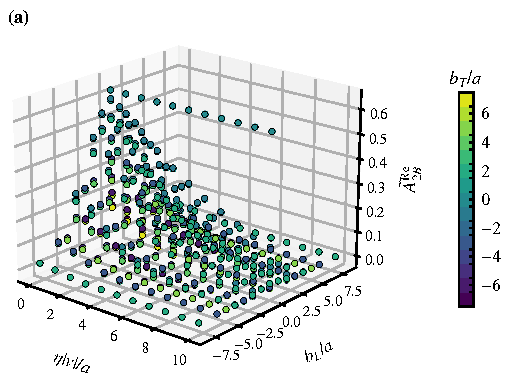
\includegraphics[width=\panelw]{figures/panels/amps/amp3d_ReA2B_PL3.pdf}\hfill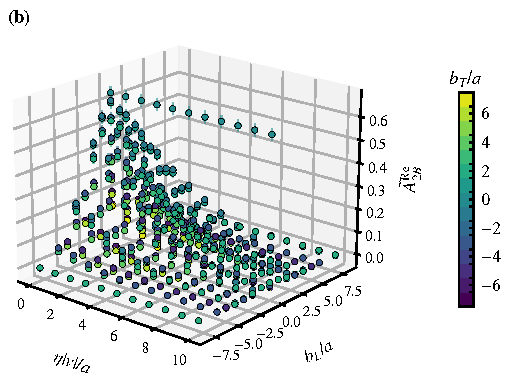
\includegraphics[width=\panelw]{figures/panels/amps/amp3d_ReA2B_PL4.pdf}\par
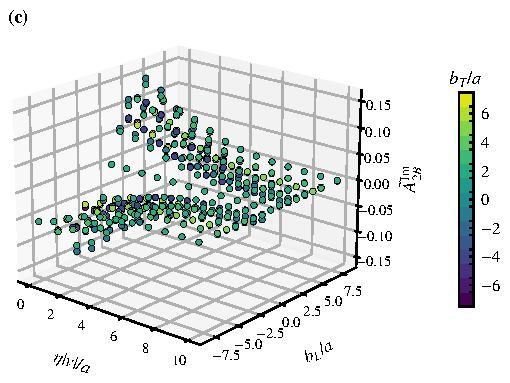
\includegraphics[width=\panelw]{figures/panels/amps/amp3d_ImA2B_PL3.pdf}\hfill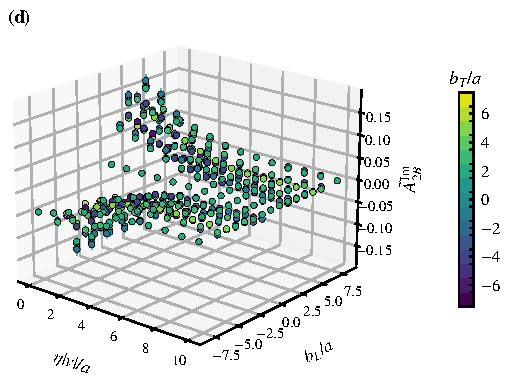
\includegraphics[width=\panelw]{figures/panels/amps/amp3d_ImA2B_PL4.pdf}\par
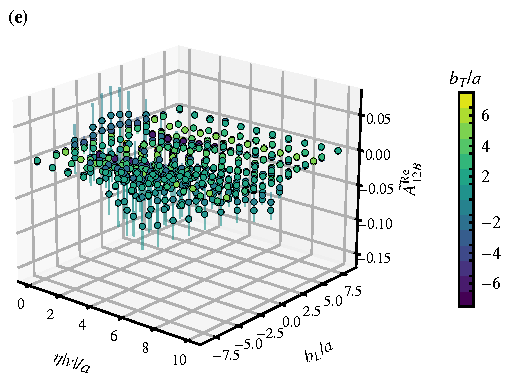
\includegraphics[width=\panelw]{figures/panels/amps/amp3d_ReA12B_PL3.pdf}\hfill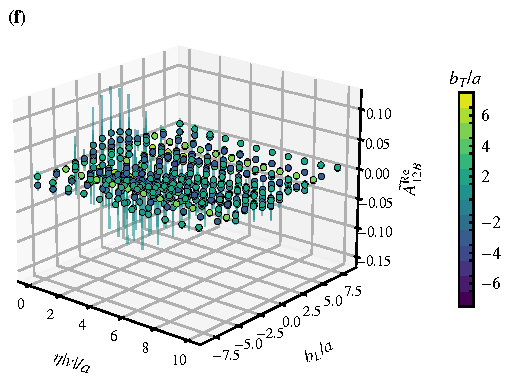
\includegraphics[width=\panelw]{figures/panels/amps/amp3d_ReA12B_PL4.pdf}
\caption{As Fig.~\ref{fig:BLBT_3D_P1} for $\vect{P}\cdot a\hat{L}/(2\pi)=\{-3,0,0\}$ ($\hat\zeta=0.539684$, left) and $\{-4,0,0\}$ ($\hat\zeta=0.785756$, right), rows: $\tAmp_{2B}^{\text{Re}}$, $\tAmp_{2B}^{\text{Im}}$, $\tAmp_{12B}^{\text{Re}}$.}
\label{fig:BLBT_3D_P3}
\end{figure*}

\begin{figure*}[!p]
\centering
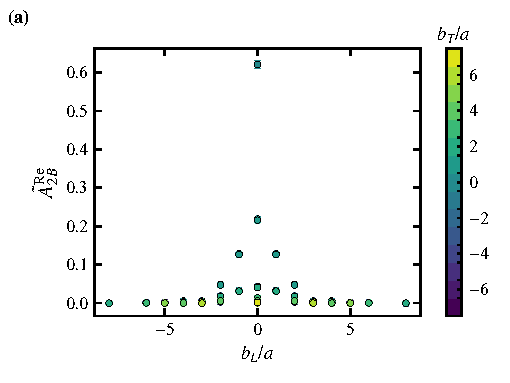
\includegraphics[width=\panelw]{figures/panels/amps/amp2d_eta8_ReA2B_PL3.pdf}\hfill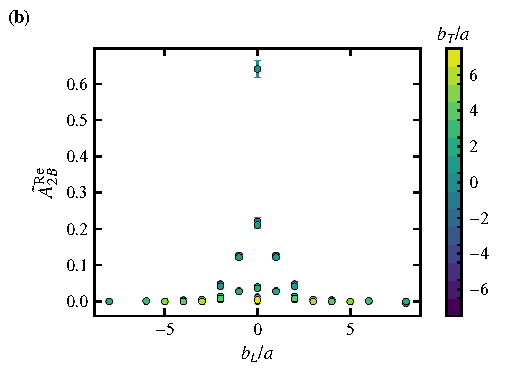
\includegraphics[width=\panelw]{figures/panels/amps/amp2d_eta8_ReA2B_PL4.pdf}\par
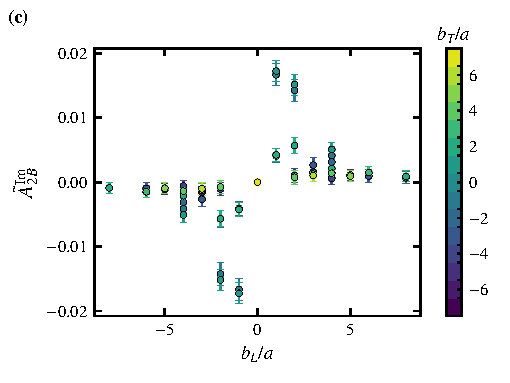
\includegraphics[width=\panelw]{figures/panels/amps/amp2d_eta8_ImA2B_PL3.pdf}\hfill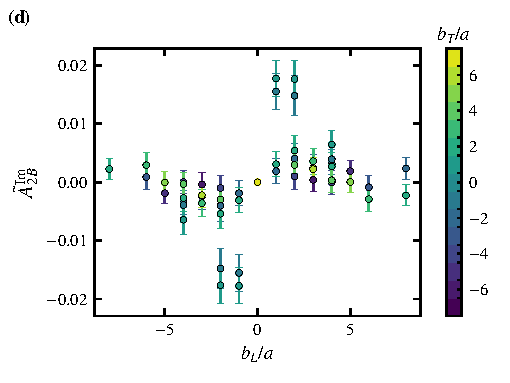
\includegraphics[width=\panelw]{figures/panels/amps/amp2d_eta8_ImA2B_PL4.pdf}\par
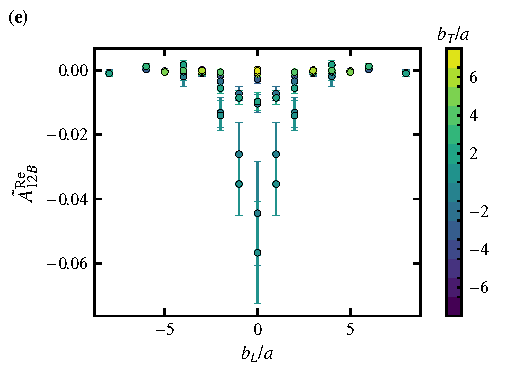
\includegraphics[width=\panelw]{figures/panels/amps/amp2d_eta8_ReA12B_PL3.pdf}\hfill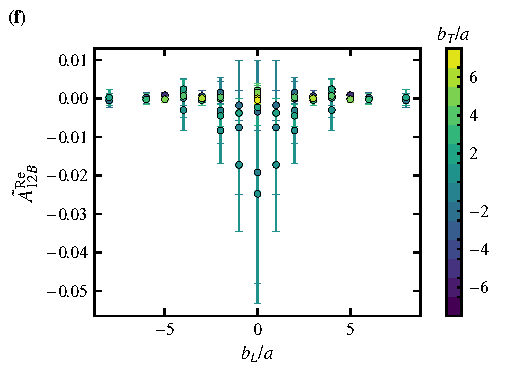
\includegraphics[width=\panelw]{figures/panels/amps/amp2d_eta8_ReA12B_PL4.pdf}
\caption{As Fig.~\ref{fig:BLBT_eta8_P1} for $\vect{P}\cdot a\hat{L}/(2\pi)=\{-3,0,0\}$ ($\hat\zeta=0.539684$, left) and $\{-4,0,0\}$ ($\hat\zeta=0.785756$, right), rows: $\tAmp_{2B}^{\text{Re}}$, $\tAmp_{2B}^{\text{Im}}$, $\tAmp_{12B}^{\text{Re}}$.}
\label{fig:BLBT_eta8_P3}
\end{figure*}

\begin{figure*}[!t]
\centering
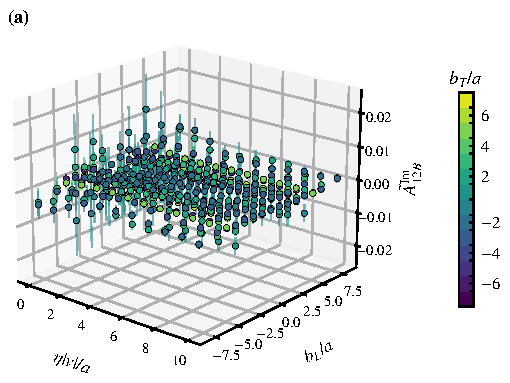
\includegraphics[width=\panelw]{figures/panels/amps/amp3d_ImA12B_PL3.pdf}\hfill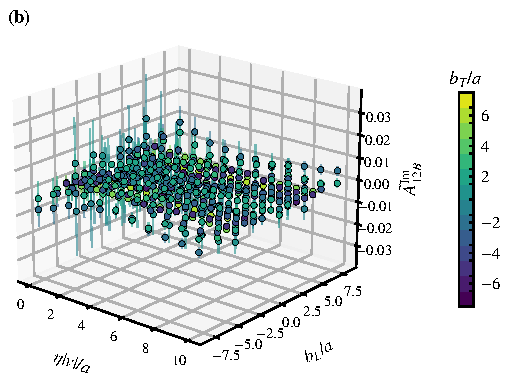
\includegraphics[width=\panelw]{figures/panels/amps/amp3d_ImA12B_PL4.pdf}\par
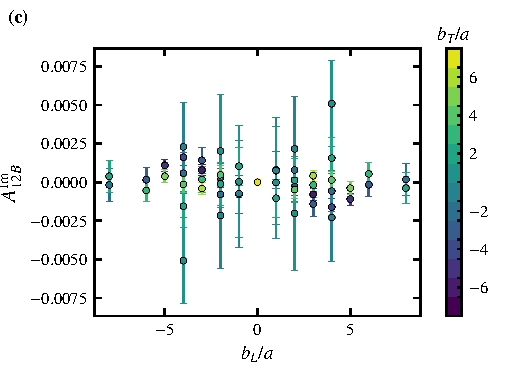
\includegraphics[width=\panelw]{figures/panels/amps/amp2d_eta8_ImA12B_PL3.pdf}\hfill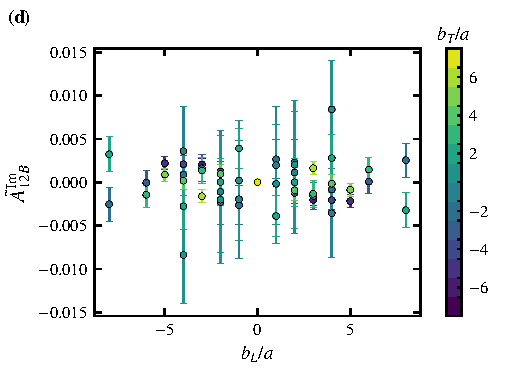
\includegraphics[width=\panelw]{figures/panels/amps/amp2d_eta8_ImA12B_PL4.pdf}
\caption{$\tAmp_{12B}^{\text{Im}}$ for $\vect{P}\cdot a\hat{L}/(2\pi)=\{-3,0,0\}$ ($\hat\zeta=0.539684$, left) and $\{-4,0,0\}$ ($\hat\zeta=0.785756$, right): as functions of $\eta|\vect v|/a$ and $b_L/a$ (top) and of $b_L/a$ at $\eta|\vect v|/a=8$ (bottom).}
\label{fig:BLBT_ImA12B_P34}
\end{figure*}


\bibliography{refs}

\end{document}
